% \documentstyle[amsmath,epic,eepic,graphicx,tabularx,cite,subfig,caption,appendix,algorithm,algorithmicx,algpseudocode,amssymb,listings,color,afterpage]{poly3}
\documentstyle[epic,eepic,graphicx,tabularx,multirow,mathtools,cite,subfig,caption,appendix,algorithm,algorithmicx,algpseudocode,amssymb,listings,color,afterpage, placeins]{poly3}
%\mathindent 0pt

%%% Use includeonly to pdf only one chapter %%% <-------------------------------------------------------------------------------------------------------------
\includeonly{./chapters/results_navigation}
% \includeonly{./chapters/results_crawl}

%\documentclass{report}[10pt]
%\usepackage{fancyhdr}
%\usepackage{amssymb}
%\usepackage{geometry}
%\usepackage{makecell}
%\usepackage[pdftex]{graphicx}
%\usepackage{mathtools}
%\usepackage{multicol}
%\usepackage[mathscr]{euscript}
%\usepackage[toc,page]{appendix}
%\usepackage[T1]{fontenc}
%\usepackage{titlesec, blindtext, color}
%\usepackage{framed}
%\usepackage{color}
%\usepackage{listings}
%\usepackage{dsfont}
%\usepackage{subcaption}
%\usepackage{natbib}
%\usepackage{tabularx}
%\usepackage[table]{xcolor}
%\usepackage{fullpage}
\newcolumntype{L}[1]{>{\hsize=#1\hsize\raggedright\arraybackslash}X}
\newcolumntype{R}[1]{>{\hsize=#1\hsize\raggedleft\arraybackslash}X}
\newcolumntype{C}[1]{>{\hsize=#1\hsize\centering\arraybackslash}X}

% Format Parameters
%\setlength{\parskip}{14pt plus 4pt minus 4pt}
%\linespread{1.125}

\newcommand{\col}[2]{\text{col}(#1)_{#2}}
\newcommand{\wrap}[1]{\left(#1\right)}
\newcommand{\sbrack}[1]{\left[#1\right]}
\newcommand{\setwrap}[1]{\left\{#1\right\}}
\newcommand{\abs}[1]{\left\lVert#1\right\rVert}
\newcommand{\norm}[1]{\left\lVert#1\right\rVert}
\newcommand{\ciel}[1]{\left\lceil#1\right\rceil}
%\definecolor{gray75}{gray}{0.75}

\newcommand{\mmathcal}[1]{{\cal #1}}
\newcommand{\mmathbb}[1]{{\Bbb #1}}

\newcommand{\Bellman}{T_{\gamma}^{\pi}}
\newcommand{\BellmanOpt}{T_{\gamma}^{*}}
\newcommand{\BellmanPiOpt}{T_{\gamma}^{\pi^{*}}}
\newcommand{\expect}[1]{\emph{E}\left[#1\right]}
\newcommand{\condexpect}[2]{\expect{#1 \middle\vert #2 }}
\newcommand{\expw}[1]{\exp\wrap*{#1}}
\newcommand{\Ssize}{\abs{S}}
\newcommand{\Asize}{\abs{A}}
\newcommand{\OptV}{V^{*}}
\newcommand{\Vpi}{V^{\pi}}
\newcommand{\OptPi}{\pi^{*}}
\newcommand{\OptVpi}{V^{\OptPi}}
\newcommand{\Aspace}{\mathcal{A}}
\newcommand{\Sspace}{\mathcal{S}}
\newcommand{\linedsection}[1]{\section*{#1}\vspace{-8mm}\hrulefill}
\newcommand{\hsp}{\hspace{20pt}}
\newcommand{\ith}{\hspace{0.1mm}$i^{th}$}
\newcommand{\jth}{\hspace{0.1mm}$j^{th}$}
\newcommand{\kth}{\hspace{0.1mm}$k^{th}$}
\newcommand{\Ith}{\hspace{0.1mm}$i^{th}$\hspace{0.5mm}}
\newcommand{\Jth}{\hspace{0.1mm}$j^{th}$\hspace{0.5mm}}
\newcommand{\Kth}{\hspace{0.1mm}$k^{th}$\hspace{0.5mm}}
\newcommand{\Forall}{\hspace{1mm}\forall\hspace{1mm}}
\newcommand{\SmallThenNormal}[1]{#1}
\newcommand{\RealVec}[1]{\in \emph{R}^{#1}}
\newcommand{\RealMat}[2]{\in \emph{R}^{#1\times#2}}
\newcommand{\Real}{\Re}
\newcommand{\RRe}{\mmathcal{R}}
\newcommand{\RRealVec}[1]{\in \RRe^{#1}}
\newcommand{\RRealMat}[2]{\in \RRe^{#1\times#2}}
\newcommand{\RReal}{\RRe}
\newcommand{\InRe}[1]{\in\RReal^{#1}}
\newcommand{\EqRef}[1]{Equation \ref{eq:#1}}
\newcommand{\EqLabel}[1]{\label{eq:#1}}
\newcommand{\FigRef}[1]{Figure \ref{fig:#1}}
\newcommand{\FigLabel}[1]{\label{fig:#1}}
\newcommand{\TableRef}[1]{Table \ref{tab:#1}}
\newcommand{\TableLabel}[1]{\label{tab:#1}}
\newcommand{\Sep}{\hspace{5mm}}
\newcommand{\SSep}{\hspace{2mm}}
\newcommand{\IE}{\emph{i.e.},\hspace{1mm}}
\newcommand{\EG}{\emph{e.g.},\hspace{1mm}}
\newcommand{\DotProd}[2]{\DotBrack*{#1,#2}}
\newcommand{\DiagMat}[1]{\text{diag}\wrap{#1}}
\newcommand{\Maps}[3]{ #1 \hspace{2mm} \Real^{#2} \rightarrow \Real^{#3}}
\newcommand{\Normalize}[1]{\frac{#1}{\norm{#1}}}
\newcommand{\Sig}[1]{\text{sig}\wrap{#1}}
\newcommand{\Unit}[1]{\emph{U}\wrap{#1}}
\newcommand{\Skew}[1]{\emph{S}\wrap{#1}}
\newcommand{\ForI}{ \forall i \in \SetWrap*{1,2,3,4} }
\newcommand{\Half}{0.5}
\newcommand{\Where} {\noindent where}
\newcommand{\SectionLabel}[1]{\label{sec:#1}}
\newcommand{\SectionRef}[1]{Section \ref{sec:#1}}
\newcommand{\SectionRefH}[1]{Section #1}
\newcommand{\SectionsRefH}[1]{Sections #1}
\newcommand{\SectionHead}[1]{\normalsize}
\newcommand{\SectionTail}[1]{\SectionLabel{#1}\normalsize}
\newcommand{\Project}[2]{{P}_{#2}\wrap{#1}}
%\newcommand{\Markup}[1]{ {\noindent\color{red}#1} }
\newcommand{\Markup}[1]{#1}
\newcommand{\NeedsRef}[1]{\Markup{Needs Ref : \emph{#1}}}
\newcommand{\MissingRef}{\Markup{[*]}}
\newcommand{\MissingFig}{\Markup{[NEED FIG]}}
\newcommand{\CaseIf}{ \text{if}\hspace{1mm}}
\newcommand{\Sum}[3]{\sum_{#1=#2}^{#3}}
\newcommand{\Para}[1]{\indent{#1}\\}
\newcommand{\R}[2]{R_{#1}\wrap{#2}}
\newcommand{\SQuotes}[1]{`#1'}
\newcommand{\DQuotes}[1]{``#1''}
\newcommand{\InlineSeg}{\SSep , \SSep}
\newcommand{\convhull}[1]{\text{conv}\wrap{#1}}
\newcommand{\zcomp}[1]{\sbrack{#1}_{z}}
\newcommand{\ycomp}[1]{\sbrack{#1}_{y}}
\newcommand{\xcomp}[1]{\sbrack{#1}_{x}}


%% Image Settings
\newcommand{\ImageWidthRatio}{1.00}
\newcommand{\ImageWidthRatioSmall}{0.400}
\newcommand{\ImageWidthRatioSub}{0.950}
\newcommand{\ImagePostNoGap}{\vspace{-2mm}}
\newcommand{\SetImage}[2]{\fbox{\includegraphics[width=#1\textwidth]{#2}}}


% Equations
%\DeclareMathSizes{4}{4}{2}{2}


% Title Formatting
%\titleformat{\chapter}{\vspace{-40mm}\Huge\bfseries}{\thechapter\hsp\textcolor{gray75}{|}\hsp}{0pt}{\Huge\bfseries}


\input{epsf}

% Override the double parenthesis
\newtagform{defaultoveride}{}{}
\usetagform{defaultoveride}

% Set default code formatting scheme
\usepackage{listings}
\usepackage{color}

\definecolor{mygreen}{rgb}{0,0.6,0}
\definecolor{mygray}{rgb}{0.5,0.5,0.5}
\definecolor{mymauve}{rgb}{0.58,0,0.82}

\lstset{ %
  backgroundcolor=\color{white},   % choose the background color; you must add \usepackage{color} or \usepackage{xcolor}
  basicstyle=\footnotesize,        % the size of the fonts that are used for the code
  breakatwhitespace=false,         % sets if automatic breaks should only happen at whitespace
  breaklines=true,                 % sets automatic line breaking
  captionpos=b,                    % sets the caption-position to bottom
  commentstyle=\color{mygreen},    % comment style
  deletekeywords={...},            % if you want to delete keywords from the given language
  escapeinside={\%*}{*)},          % if you want to add LaTeX within your code
  extendedchars=true,              % lets you use non-ASCII characters; for 8-bits encodings only, does not work with UTF-8
  frame=single,                    % adds a frame around the code
  keepspaces=true,                 % keeps spaces in text, useful for keeping indentation of code (possibly needs columns=flexible)
  keywordstyle=\color{blue},       % keyword style
  language=C++,                 % the language of the code
  morekeywords={*,...},            % if you want to add more keywords to the set
  numbers=left,                    % where to put the line-numbers; possible values are (none, left, right)
  numbersep=5pt,                   % how far the line-numbers are from the code
  numberstyle=\tiny\color{mygray}, % the style that is used for the line-numbers
  rulecolor=\color{black},         % if not set, the frame-color may be changed on line-breaks within not-black text (e.g. comments (green here))
  showspaces=false,                % show spaces everywhere adding particular underscores; it overrides 'showstringspaces'
  showstringspaces=false,          % underline spaces within strings only
  showtabs=false,                  % show tabs within strings adding particular underscores
  stepnumber=2,                    % the step between two line-numbers. If it's 1, each line will be numbered
  stringstyle=\color{mymauve},     % string literal style
  tabsize=2,                       % sets default tabsize to 2 spaces
  title=\lstname                   % show the filename of files included with \lstinputlisting; also try caption instead of title
}
% Set path for images
\graphicspath{{./pictures/}}


%%%%%%%%%%%%%%%%%%%%%%%%%%%%%%%%%%%%%%%%%%%%%%%%%%%
\renewcommand{\baselinestretch}{1.6}
\newtheorem{theorem}{Theorem}[chapter]
\newcommand{\btheorem}{\begin{theorem}\rm}
\newcommand{\etheorem}{$\diamond$\end{theorem}}
\newtheorem{definition}{Definition}[chapter]
\newcommand{\bdefn}{\begin{definition}\rm}
\newcommand{\edefn}{\end{definition}}
\newtheorem{lemma}{Lemma}[chapter]
\newtheorem{remark}{Remark}[chapter]
\newcommand{\bremark}{\begin{remark}\rm}
\newcommand{\eremark}{\end{remark}}
\newtheorem{example}{Example}[chapter]
\newcommand{\bexample}{\begin{example}\rm}
\newcommand{\eexample}{\end{example}}
\newtheorem{assumption}{Assumption}[chapter]
\newcommand{\bassump}{\begin{assumption}\rm}
\newcommand{\eassump}{\end{assumption}}

\begin{document}
%%% Comment out below when pdfing only one chapter %%% <-------------------------------------------------------------------------------------------------------------
% \title{DOING THINGS WITH THE NAO :\\LIKE LASERS AND STUFF}
% \author{Griswald Brooks}
% \date{July, 2015}
% \committee{1}

% \mstitlepage
%%% Comment out above when pdfing only one chapter %%% <-------------------------------------------------------------------------------------------------------------

\topmargin=0.4in
\textwidth=6.0in
\textheight=9.0in


%%%%%%%%%%%%%%%%%%%%%%%%%%%%%%%%%%%%%%%%%%%%%%%%%%%

%%% I think this is how it's going to be laid out %%
% Abstract
% Chapter 1 Introduction
% Chapter 2 Nao Humanoid Platform
%  Hardware, Software, SDK
% Chapter 3 Navigation 
% Chapter 4 Path Planning and Obstacle Avoidance
%  GODZILA, Multi Gait Planner, SFM, SLAM...
% Chapter 5 Projected Profile Gait
%  Gaiting problem, formulation, optimization structure
% Chapter 6 Experimental Results
% Chapter 7 Conclusion
% References
%%%

%%% About me and Abstract
%%%%%%%%%%%%%%%%%%%%%%%%%%%%%%%%%%%%%%%%%%%%%%%%%%%
\setcounter{page}{1}
\pagenumbering{roman}
\chapter*{VITA}
\setcounter{page}{2}
	\vitaentry{Dec, 1983}{Born}
	\vitaentry{Jun, 2001}{Graduated from Inter-Lakes High School.}

	\vitaentry{Sep, 2001}{Enlisted into the US Navy to be trained as an Electronics Technician.}
	\vitaentry{Dec, 2007}{Seperated from US Navy with Honorable Discharge.}
	
	\vitaentry{Jan, 2007}{Entered the Lakes Region Community College as a Computer Technologies major.}
	\vitaentry{May, 2010}{Received AS Degree from the Lakes Region Community College.}

	\vitaentry{Jan, 2010}{Entered the Polytechnic Institute of NYU as a Computer Engineering major.}
	\vitaentry{May, 2013}{Received BS Degree cum laude from the Polytechnic Institute of NYU.}

	\vitaentry{Jan, 2014}{Entered the NYU Polytechnic School of Engineering as a Electrical Engineering major.}
	\vitaentry{May, 2015}{Received MS Degree from the NYU Polytechnic School of Engineering.}

	\vitaentry{Dec, 2065}{Deceased due to Robot Apocalypse.}
\include{./chapters/publications}
\clearpage
%\chapter*{Acknowledgments}
\vspace*{\fill}
	\begin{center}
		\begin{minipage}{\textwidth}
			{\begin{center}{\textbf{ACKNOWLEDGEMENTS}}\end{center}\vspace{10mm}}
			Thank Khorrami
			
			\vspace{5mm}
			\hspace{5mm} 
			Thank PK, Brian, and Agraj.
		\end{minipage}
	\end{center}
\vfill % equivalent to \vspace{\fill}
\clearpage

\clearpage
\vspace*{\fill}
	\begin{center}
		\begin{minipage}{\textwidth}
		\emph{
				Dedicate to Mom and Dad. I totally wouldn't have even gone to this school if not for my Dad.
			}
		\end{minipage}
	\end{center}
\vfill % equivalent to \vspace{\fill}
\clearpage
{\msabstract{Dr. Farshad Khorrami}}
{
	This thesis shows what I did over the course of two years. I did something with the Nao robot and made it move and look at things and stuff.
	You'll see.
\clearpage}
{\endmsabstract}

\normalsize
%%% Comment out below when pdfing only one chapter %%% <-------------------------------------------------------------------------------------------------------------
% \tableofcontents
% \listoffigures
% \listoftables
%%% Comment out above when pdfing only one chapter %%% <-------------------------------------------------------------------------------------------------------------
\newpage
\setcounter{page}{1}
\pagenumbering{arabic}

%%% Thesis go!
%%%%%%%%%%%%%%%%%%%%%%%%%%%%%%%%%%%%%%%%%%%%%%%%%%%
	%%%%%%%%%%%%%%%%%%%%%%%%%%%%%%%%%%%%%%%%%%%%%%%%%%%%%%%%%%%%%%%%%%%%%%%%%%%%%%%%%%
%%% Introduction
%%%
%%% What are we trying to get done?
%%% How to we tackle the problem?
%%% Why did we use this approach?
%%% Why did we use this platform?
%%%
%%% Section 1 : Concept and Motivation
%%% Section 2 : Platform Overview
%%% Section 3 : Problem Domain
%%% Section 4 : Implemented Components
%%%		SubSection 4.1 : Navigation
%%% 	SubSection 4.2 : Crawlspace Detector	
%%%		SubSection 4.3 : Crawl Gait
%%% Section 5 : Thesis Structure
%%%
%%%%%%%%%%%%%%%%%%%%%%%%%%%%%%%%%%%%%%%%%%%%%%%%%%%%%%%%%%%%%%%%%%%%%%%%%%%%%%%%%%
\chapter{Introduction} \label{ch::introduction}

\section{Concept and Motivation}
% We are trying to make things that help the robot get from A to B.
% The problem of getting the robot from A to B looks like this: stuff, stuff, stuff.
A common task for robotic systems is for a mobile platform to transport itself from one location to another
in the presence of environmental obstacles. Within this general task there are many subproblems. The system
must have some sort of awareness of the destination objective and usually some notion of where it is relative
to that destination. The destination location and the location of the robot can be encoded in a map that
the mobile platform or some off board system is responsible for maintaining. Within the environment there may 
be obstacles that prevent the robot from moving through that space which can also be encoded into the map. 
Given these notions of robot, goal, and obstacle locations often an initial path is planned to allow the robot
to reach the goal location. In addition to these higher level concepts, the robot must have a scheme by which it
transports itself through the environment be rolling, walking, flying and controls for each of those methods.
Solutions to these subproblems, map building, robot localization, obstacle localization,
path planning, locomoting and others work together to accomplish the overall goal. 
Each of these subproblems can be expanded upon and this thesis works on three of these components: 
local navigation, obstacle detection and characterization, and gaiting. Used to work on these problems
was the Nao Humanoid Platform by Aldebaran Robotics.

\begin{figure}[h!]
	\centering
	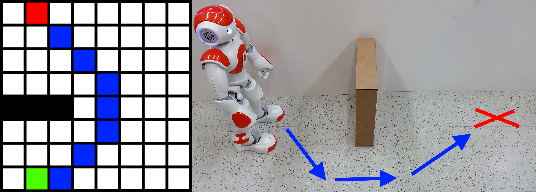
\includegraphics{nao_with_obstacle_and_map1.png}
	\caption
	{Example illustration of the Nao humanoid robot in an environment with an obstacle. The red X represents a goal
		location with the blue arrows showing an possible path. On the left side is one possible representation
		of the environment as a 2D grid.}
	\label{fig:nao_with_map1}
\end{figure}


\section{Platform Overview}
% As a medium we worked with the Nao. The Nao is good because this: stuff, stuff, stuff.
The broader task of moving an agent from one location to another is applicable to a wide range of robots but
each platform will have details that change the scope of the problem and the method used to approach it.
The three problems focused on (local navigation, obstacle detection, and gaiting) for a flying robot with 
a global camera system will require different solutions than a wheeled robot with only rangefinders.
For this thesis, the Nao H25 V4 Humanoid Platform by Aldebaran Robotics was chosen to act as the mobile base. 
With the future goal of having robots interact in human environments, humanoid platforms have become an active
area of research as they are physically compatible with such environments. 
While Nao is a 1.9 ft tall humanoid weighing 9.5 lbs and therefore only an appropriate analog for a young human toddler,
the humanoid format is of primary importance to algorithmic development.
with 25 degrees of freedom including two legs, two arms, and two grippers. 
Figure \ref{fig:nao_diagram1} shows a cursory illustration of the humanoid configuration.
This lightweight but capable configuration enables research into mobile manipulation, humanoid gaiting, and terrain adaptation
without the need for specialized support equipment such as belays or dedicated experimentation areas as the
robot is safe for humans to interact with.

\begin{figure}
	\centering
	\includegraphics[width=0.4\textwidth]{nao_coronal_highlighted2.png}
	\caption
	{Coronal view of the Nao humanoid with a few pertinent features highlighted. }
	\label{fig:nao_diagram1}
\end{figure}

The robot comes with a suite of sensors including two cameras, two ultrasonic rangefinders, 
a 3-axis accelerometer and 2-axis gyro, foot contact sensors, and angular position encoders on every joint.
Such a complement of sensors aids the robot in creating an estimate of a number of variables including 
the robot state and environment characteristics. 
Nao has a built-in WiFi radio and 1.6 GHz Intel Atom processor running a version of the Linux operating system 
allowing the robot to be programmed in C++ or Python using standard libraries that can be remotely uploaded.
These features allow the use of a wide variety of tools when constructing new algorithms and for program
iteration to happen at a rapid pace.

With all of these features the Nao makes for a convenient platform for the development of mobile robot algorithms.

% Then we stuck a Hokuyo laser on the Nao and used that for navigation. Why was this a good idea?
To augment the sensor suite, a Hokuyo URG-04LX-UG01 Scanning Laser Rangefinder (Lidar) was mounted to the Nao and
interfaced via a USB connection to the Nao's onboard computer. The sensor has a scanning area of $240^\circ$ with 
an angular resolution of $0.36^\circ$ and a range of 5 meters. It is used to generate a planar point cloud representing
the range to the nearest occlusion at a set of fixed bearing relative to the robot. Lidars are commonly used in mobile
robotics so developing algorithms utilizing them is of practical concern.

\section{Problem Domain}
% Within this, we restrict the problem to this: stuff, stuff, stuff.
The three areas selected for development were local navigation, obstacle detection and characterization, and gaiting.
Each of these is a broad research topic in its own right so the domain of investigation for each problem
must be specified. 

\section{Implemented Components}
% Within this problem well address certain components that add to our problem solving toolbox.
% These are the things we developed: thing 1, thing 2, thing 3.

\subsection{Navigation}
\subsection{Crawlspace Detector}
% Used the camera data (and gyro) to detect openings using SFM and Lidar to confirm.
\subsection{Crawl Gait}

\section{Thesis Structure}
This thesis is organized as follows: 

% Chapter \ref{ch:platform} reviews the Nao Humanoid Platform with Hokoyu Scanning Laser Rangefinder augmentation.
% The navigation system is broken into three parts, 
% Chapter \ref{ch:navigation} discusses the GODZILA algorithm used for local navigation.
% Chapter \ref{ch:detector} discusses SFM for detecting openings that the Nao might crawl under,
% Chapter \ref{ch:crawl_gait} discusses the Projected Profile crawling gait used to perform the crawl.
% Simulations and experimental results are shown in Chapters \ref{ch:simulations} and \ref{ch:results}, 
% while a discussion of the work is given in Chapter \ref{ch:conclusion}.








% Results from this work were published in \cite{our_paper1}.
% And more results were published in newer papers.


	
%%%%%%%%%%%%%%%%%%%%%%%%%%%%%%%%%%%%%%%%%%%%%%%%%%%%%%%%%%%%%%%%%%%%%%%%%%%%%%%%%%
%%% Platform Description
%%% Add sample data from cameras and lidar
%%% Section 1 : Hardware Overview
%%%		SubSection 1.1 : Pertinent Nao Statistics (and how things talk to each other)
%%% 	SubSection 1.2 : Pertinent Lidar Statistics
%%%		SubSection 1.3 : Design Requirements for Lidar Mount and Description
%%% Section 2 : Software Framework
%%%		SubSection 2.1 : NaoQi and qibuild Overview
%%% 	SubSection 2.2 : Custom Library Framework
%%%		SubSection 2.3 : User Operation
%%%
%%%%%%%%%%%%%%%%%%%%%%%%%%%%%%%%%%%%%%%%%%%%%%%%%%%%%%%%%%%%%%%%%%%%%%%%%%%%%%%%%%
\chapter{Platform} \label{ch:platform}

For this thesis we used the Nao as the mobile platform. Aldebaran makes him. He's a cool little robot and he allows us to explore both
things we wanted to look at which were navigation and gaiting. He's mobile, small, ``cost-effective"
and has a good API that we can use to do lower-level control of things when we want to, 
and abstract ourselves from it when we don't want to.
The small size means he's easy to work with.

There's definitely some more opening paragraph to be written here about the Nao.
Probably say something about why he's useful to investigate crawling. No one's going to send
Nao into a disaster zone or anything but he's not to far off from robots that you would send in
and we don't have to spend all the money or build a new lab to work with him. You can do lot's of
simulations, but in the end you still have to test on a real robot.

While the Nao is cool and all, the sonar sensors just don't cut it for what we want to do.
Lucky, Nao comes with a USB port and uses x86 and linux so it's relatively straightforward to
add new things to him.
Therefore, we added a better distance sensor. Specifically we added the Hokuyo URG-04LX-UG01.
It's a good Lidar because it has a respectable range, good angular resolution, ``cost-effective",
and is kinda lightweight.
Using this sensor we could do mapping if we wanted to which means this system is extensible to the
broader challeges of the overall navigation problem such as SLAM. Using the Lidar we'll be
able to get enough information to do the job we need to.

While it's easy to plug a USB cable into Nao's head, you still have to stick the Lidar somewhere.
Nao doesn't have mount points that make it easy to add new hardware.
Given that we have a nifty 3D printer (and I know Solidworks) we designed up a little suit of
armor for Nao with a big stick coming out of it that we could mount the Lidar to, above his head.
This works but the new dynamics destabilize Nao's default gait at certain speeds. 
This doesn't mess with the navigation algorithm, but to increase the speed this will have to be dealt with,
either by changing the rig or... using the arms to counterbalance the new inertial forces as
part of the walking gait.

\begin{figure}
  \centering
  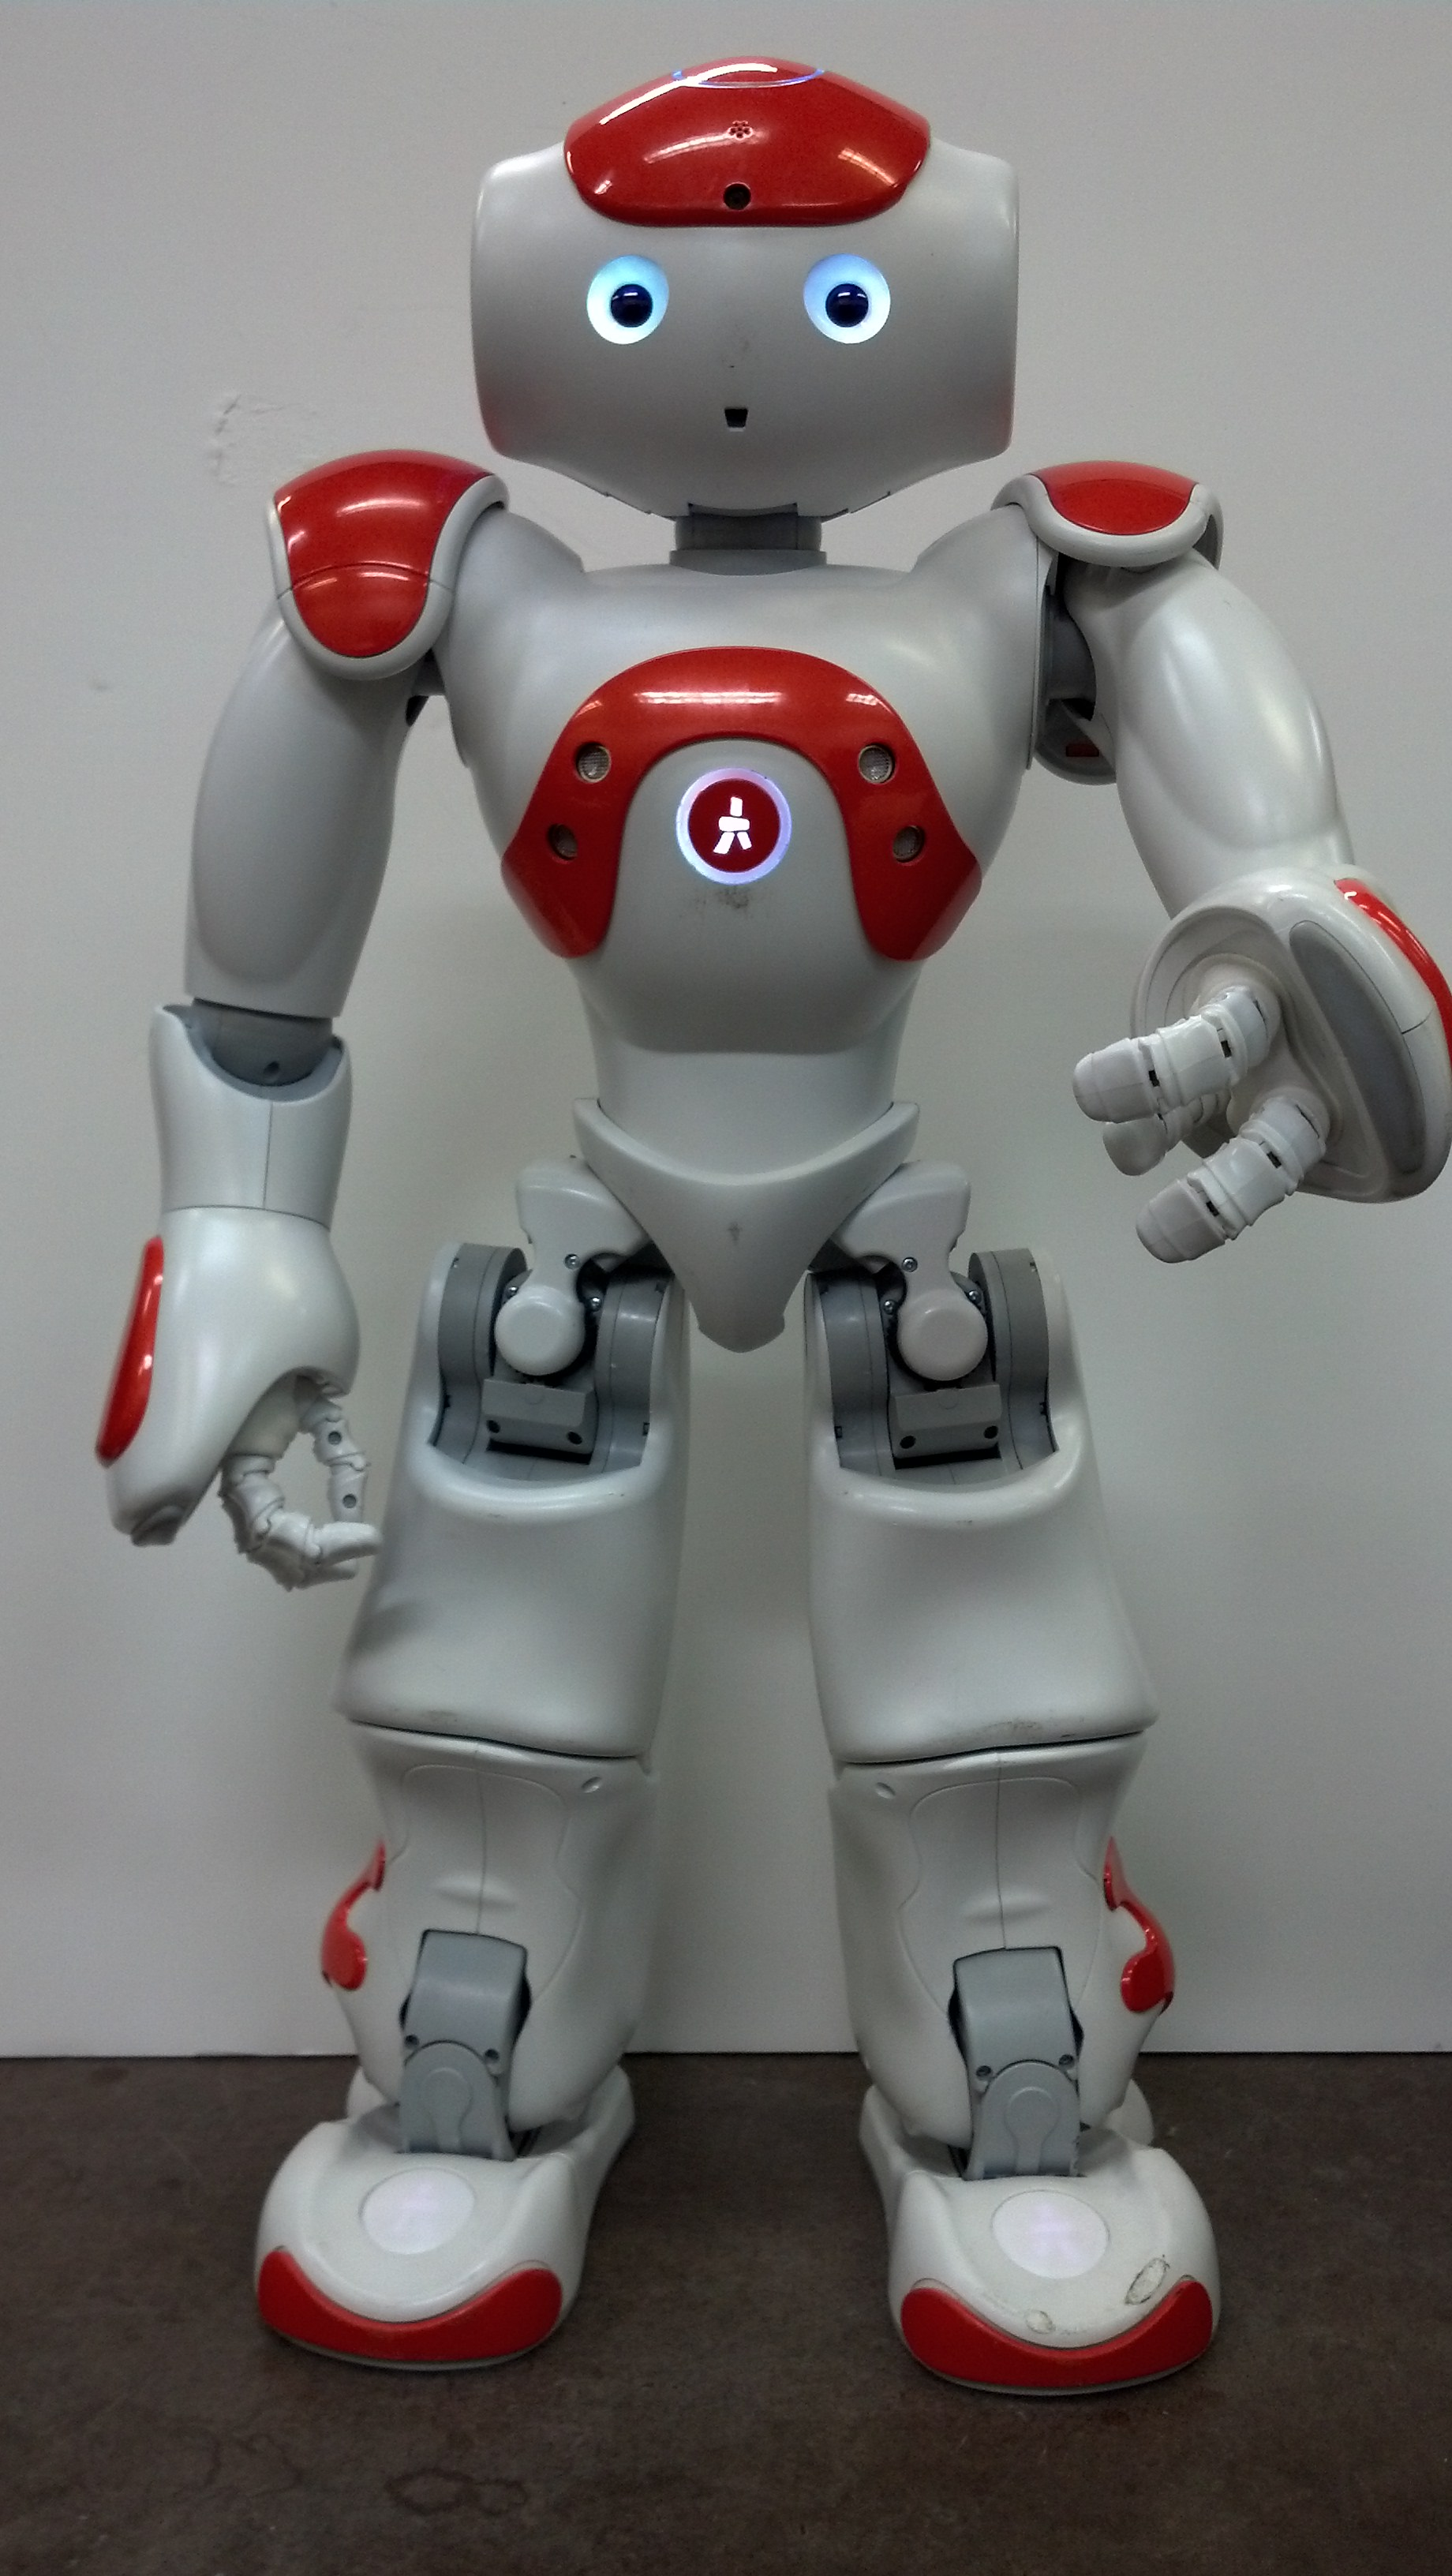
\includegraphics[height=0.4\textheight]{nao_coronal1.jpg}
  \caption{Nao at CRRL.}
  \label{fig:crrl_nao_coronal1}
\end{figure}

\begin{figure}
  \centering
  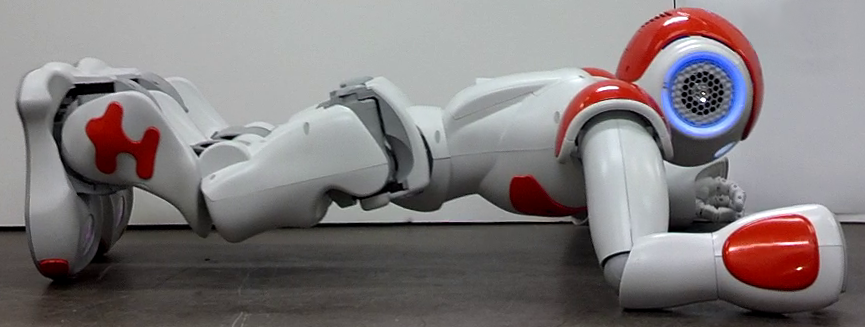
\includegraphics[width=\textwidth]{White_Background/apex_cropped.png}
  \caption{Nao in crawling pose.}
  \label{fig:crrl_nao_apex1}
\end{figure}

\begin{figure}
  \centering
  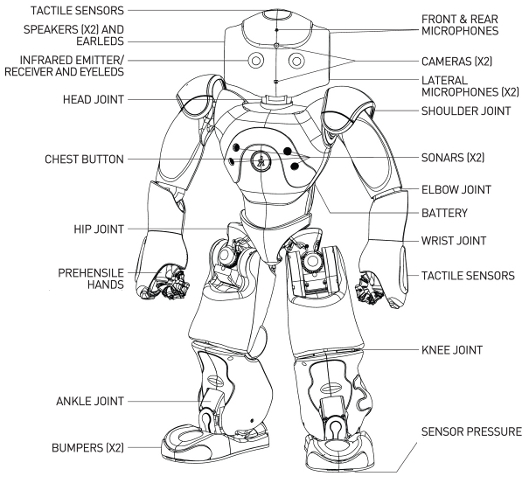
\includegraphics[width=\textwidth]{nao_diagrams/nao_h25_pres.png}
  \caption{Nao features.}
  \label{fig:nao_features1}
\end{figure}

\begin{figure}
  \centering
  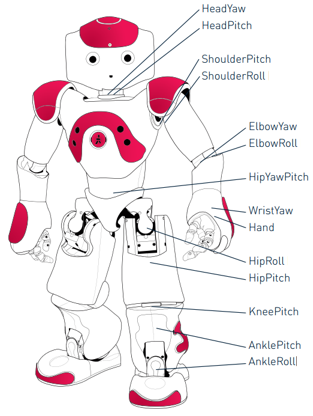
\includegraphics[height=0.4\textheight]{nao_diagrams/hardware_motortype_h25V5.png}
  \caption{Nao joints.}
  \label{fig:nao_joints1}
\end{figure}

\begin{figure}
  \centerline{
    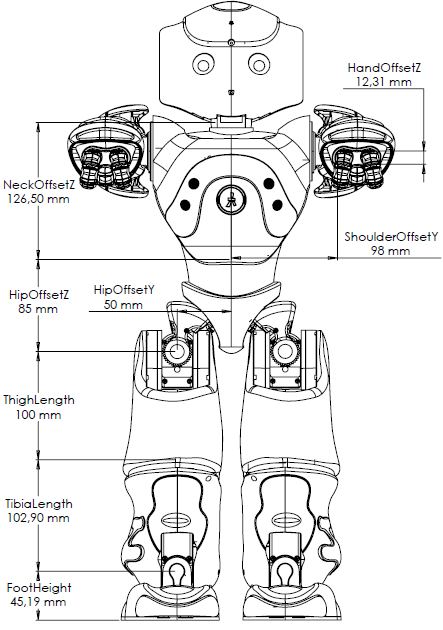
\includegraphics[width=0.45\textwidth]{nao_diagrams/hardware_lengthfront_3.3.png}
    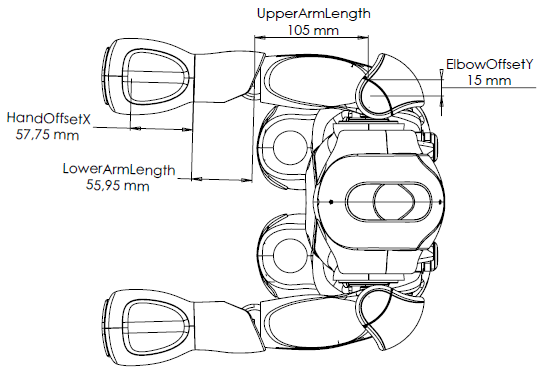
\includegraphics[width=0.55\textwidth]{nao_diagrams/hardware_lengthup_3.3.png}
  }
  \caption{Nao link lengths.}
  \label{fig:nao_link_lengths1}
\end{figure}

\begin{figure}
  \centering
  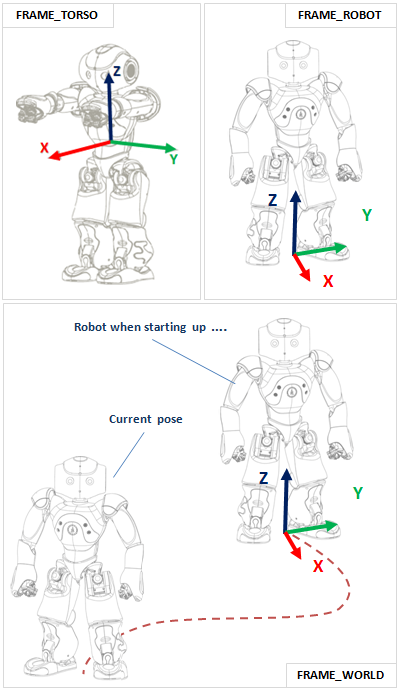
\includegraphics[height=0.75\textheight]{nao_diagrams/frame_definition_combo.png}
  \caption{Nao frames.}
  \label{fig:nao_frames1}
\end{figure}

\begin{figure}
  \centerline{
    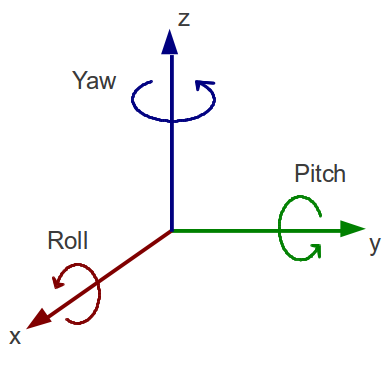
\includegraphics[width=0.5\textwidth]{nao_diagrams/rollPitchYaw.png}
  }
  \caption{Definition of roll pitch and yaw.}
  \label{fig:nao_rpy_def1}
\end{figure}

\section{Hardware Overview}
Ok so, three pieces of hardware here, the Nao, the Lidar, and the mount.
Technically, all you need is the Nao since it is a mobile base with distance sensors but the sonars
don't do that great so we added the Lidar, and since there's no where to screw it down we designed a mount.

\begin{figure}
  \centering
  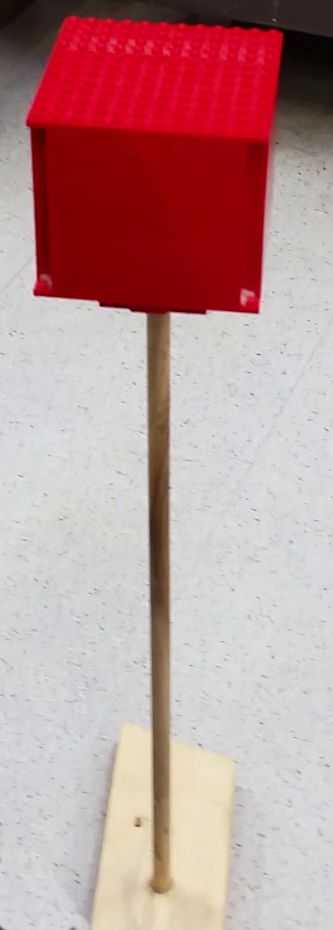
\includegraphics[height=0.4\textheight]{red_cube1.png}
  \caption{Figure showing red cube the Nao tracked.}
  \label{fig:nao_arm_joints_reflect1}
\end{figure}

\subsection{Nao Hardware}
Nao is a humanoid by Aldebaran Robotics. 25 DoF, arms, legs, head, hands feet. Sonars, joint sensors, cameras,
foot sensors, IMU, bumpers and buttons. Battery life, weight, top speed (before and after Lidar), sonar ranges, camera angles and pixels,
CPU type and speed, RAM, storage space, USB, Ethernet, WiFi.
Motor torques. (Important for Chapter \ref{ch:crawl_gait})
[Diagram of Nao. More than one to show different things]

\begin{figure}
  \centering
  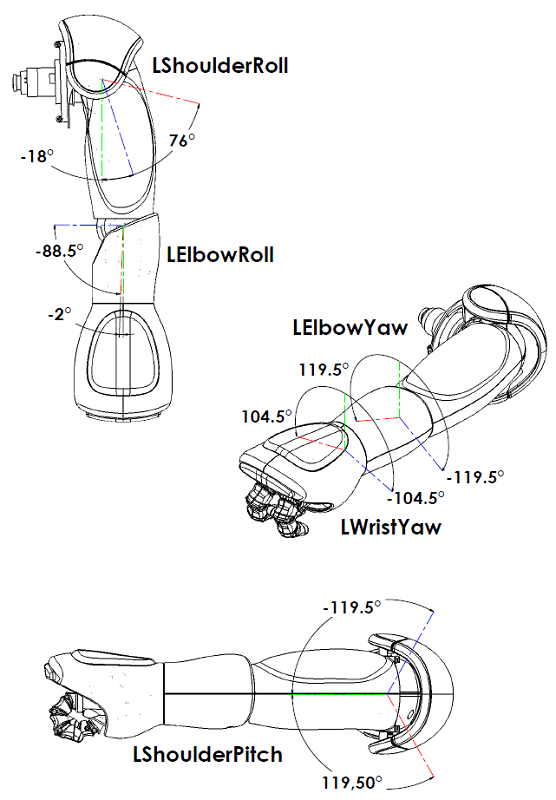
\includegraphics[width=\textwidth]{nao_diagrams/hardware_larmjoint_3.3.png}
  \caption{Figure showing left arm}
  \label{fig:nao_arm_joints_left1}
\end{figure}

\begin{figure}
  \centering
  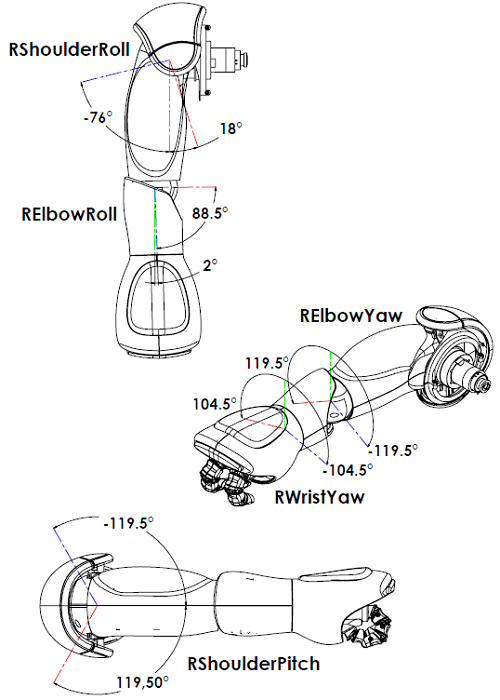
\includegraphics[width=\textwidth]{nao_diagrams/hardware_rarmjoint_3.3.png}
  \caption{Figure showing right arm}
  \label{fig:nao_arm_joints_right1}
\end{figure}

\begin{figure}
  \centering
  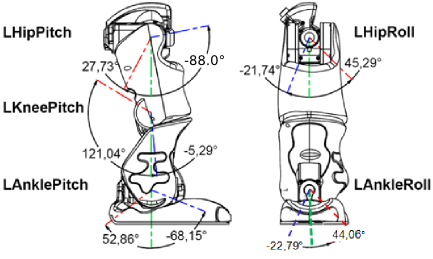
\includegraphics[width=\textwidth]{nao_diagrams/hardware_llegjoint.png}
  \caption{Figure showing left leg}
  \label{fig:nao_leg_joints_left1}
\end{figure}

\begin{figure}
  \centering
  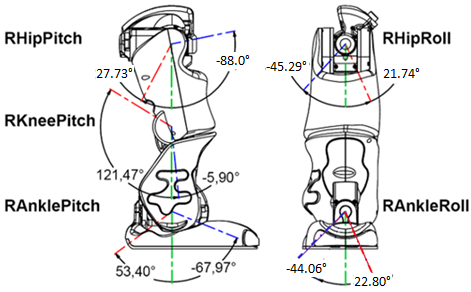
\includegraphics[width=\textwidth]{nao_diagrams/hardware_rlegjoint.png}
  \caption{Figure showing right leg}
  \label{fig:nao_leg_joints_right1}
\end{figure}

\begin{figure}
  \centering
  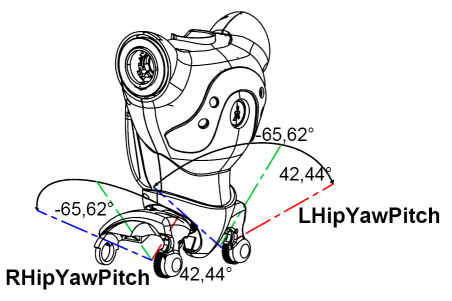
\includegraphics[width=\textwidth]{nao_diagrams/hardware_pelvisjoint.png}
  \caption{Figure showing hip yaw-pitch}
  \label{fig:nao_hip_yawpitch1}
\end{figure}


Need diagram showing arm symmetry for crawl results. 
\begin{figure}
  \centering
  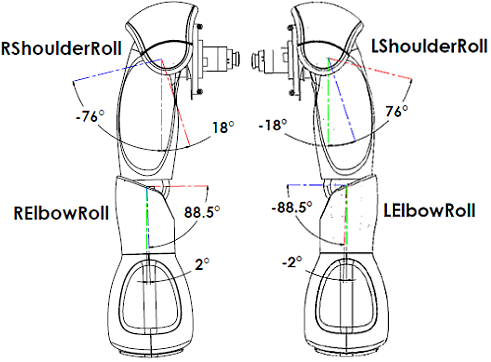
\includegraphics[width=\textwidth]{hardware_r_and_l_armjoint.png}
  \caption{Figure showing arm joints and how they are a reflection.}
  \label{fig:nao_arm_joints_reflect1}
\end{figure}

Need diagram showing different postures for crawl results. 
\begin{figure}
  \centerline{
    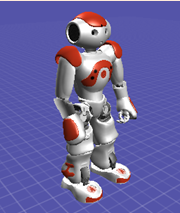
\includegraphics[width=0.33\textwidth]{posture/posture_stand.png}
    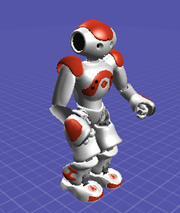
\includegraphics[width=0.33\textwidth]{posture/posture_standinit.png}
    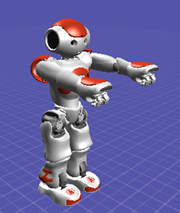
\includegraphics[width=0.33\textwidth]{posture/posture_standzero.png}
  }
  \vspace*{0.05in}
  \centerline{
    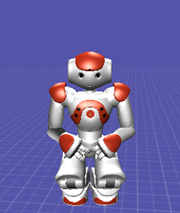
\includegraphics[width=0.33\textwidth]{posture/posture_crouch.png}
    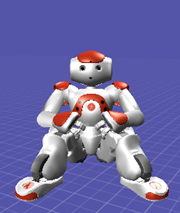
\includegraphics[width=0.33\textwidth]{posture/posture_sit.png}
    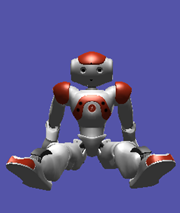
\includegraphics[width=0.33\textwidth]{posture/posture_sitrelax.png}
  }
  \vspace*{0.05in}
  \centerline{
    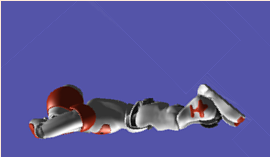
\includegraphics[width=0.5\textwidth]{posture/posture_lyingbelly.png}
    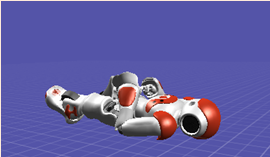
\includegraphics[width=0.5\textwidth]{posture/posture_lyingback.png}
    }
  \caption{Figure showing postures.}
  \label{fig:nao_postures1}
\end{figure}

\subsection{Lidar Hardware}
Hokuyo is a Lidar. What's a Lidar? How does it work and what does it give you? 
{Diagrams explaining things like pictures of lidar outputs}

Number of beams, angular resolution of beams, range of beams, resolution and accuracy.
Weight, power consumption, USB, update rate (sensor bandwidth).
Indoor only, not rated for outdoors.
[Diagram of Hokuyo.]

\begin{figure}
  \centering
  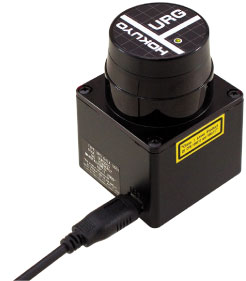
\includegraphics[height=0.4\textheight]{hokuyo/urg_04lx_ug01_top.jpg}
  \caption{Figure showing Lidar.}
  \label{fig:lidar_top1}
\end{figure}

\begin{figure}
  \centering
  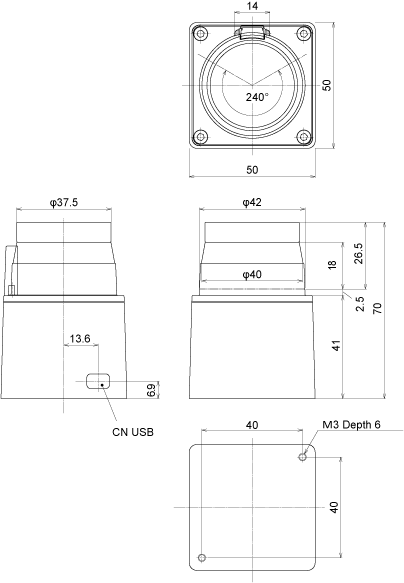
\includegraphics[height=0.4\textheight]{hokuyo/urg_04lx_ug01_ed.png}
  \caption{Figure showing Lidar.}
  \label{fig:lidar_diagram1}
\end{figure}

[Image showing angular and distance range of lidar.]
[Image showing sample lidar output.]



\subsection{Lidar Mount}
Design reqs: needed to rigidly attach to Nao for data transformation purposes, needed to see forward,
needed to be able to crawl with it, lightweight, Nao needed to be able to move his head while wearing it,
needed to be able to use the sonars (just in case).

Mounting it to the head seemed like it was going to be tough, so a vest was designed.
Straps and foam seemed like they'd hold well enough. In fact they hold so well I can lift Nao up by the mount.
[Show Solidworks design.]
\begin{figure}
  \centering
  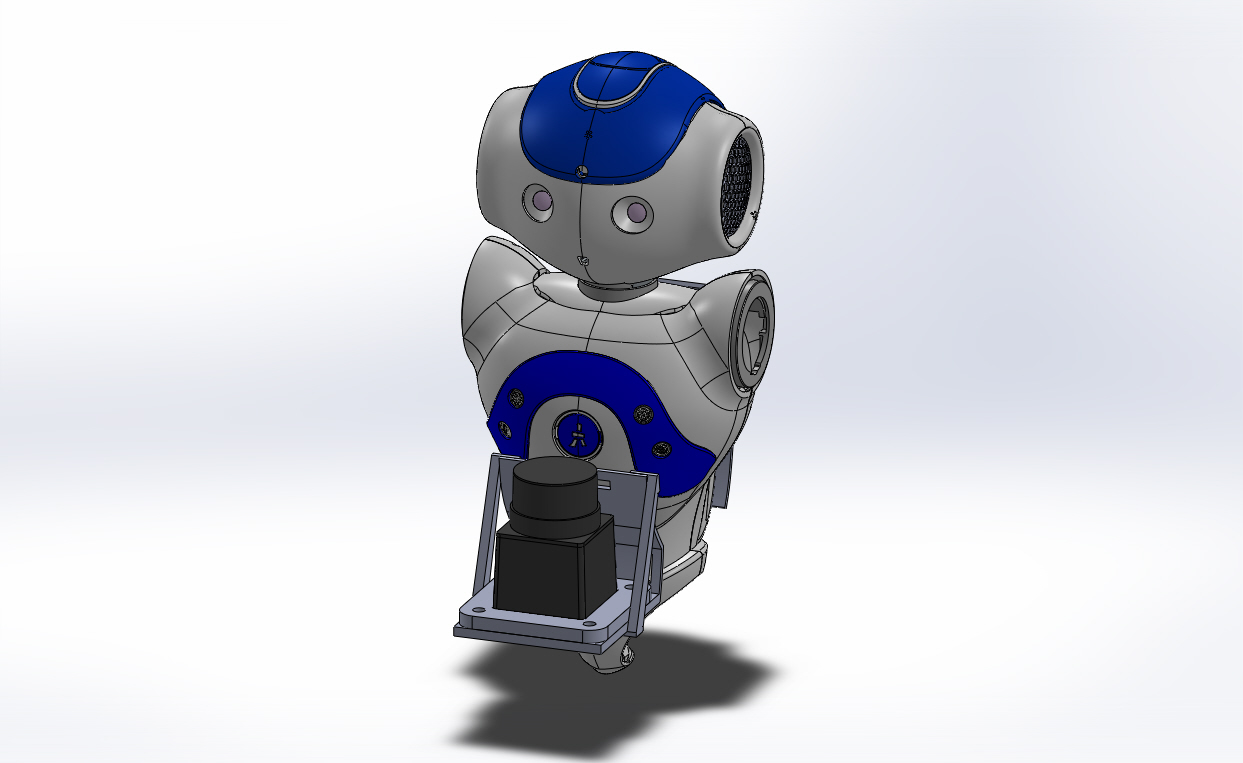
\includegraphics[height=0.4\textheight]{backpack/Assem_Nao_Dimetric1.jpg}
  \caption{Figure showing assembled Nao Lidar.}
  \label{fig:nao_lidar_mount_nao_dimetric1}
\end{figure}

\begin{figure}
  \centering
  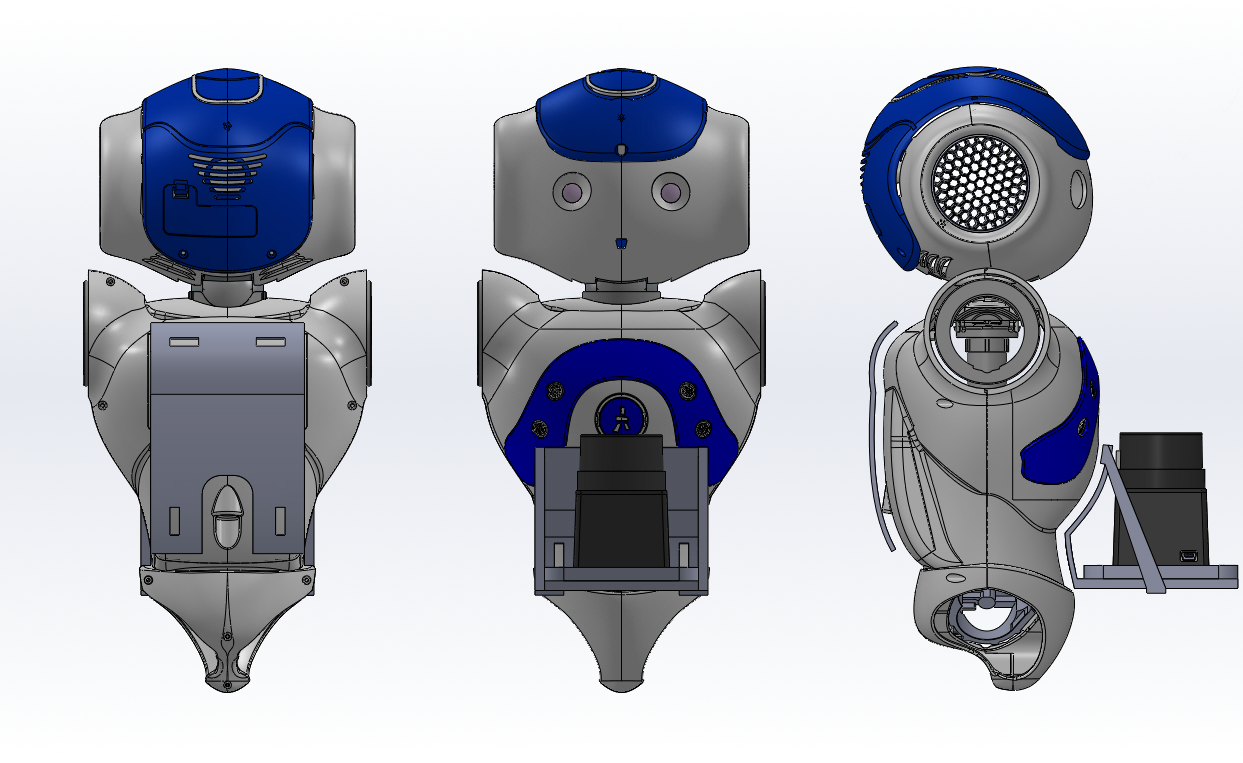
\includegraphics[height=0.4\textheight]{backpack/Assem_Nao_Three_View1.png}
  \caption{Figure showing assembled Nao Lidar.}
  \label{fig:nao_lidar_mount_nao_three_view1}
\end{figure}

\begin{figure}
  \centering
  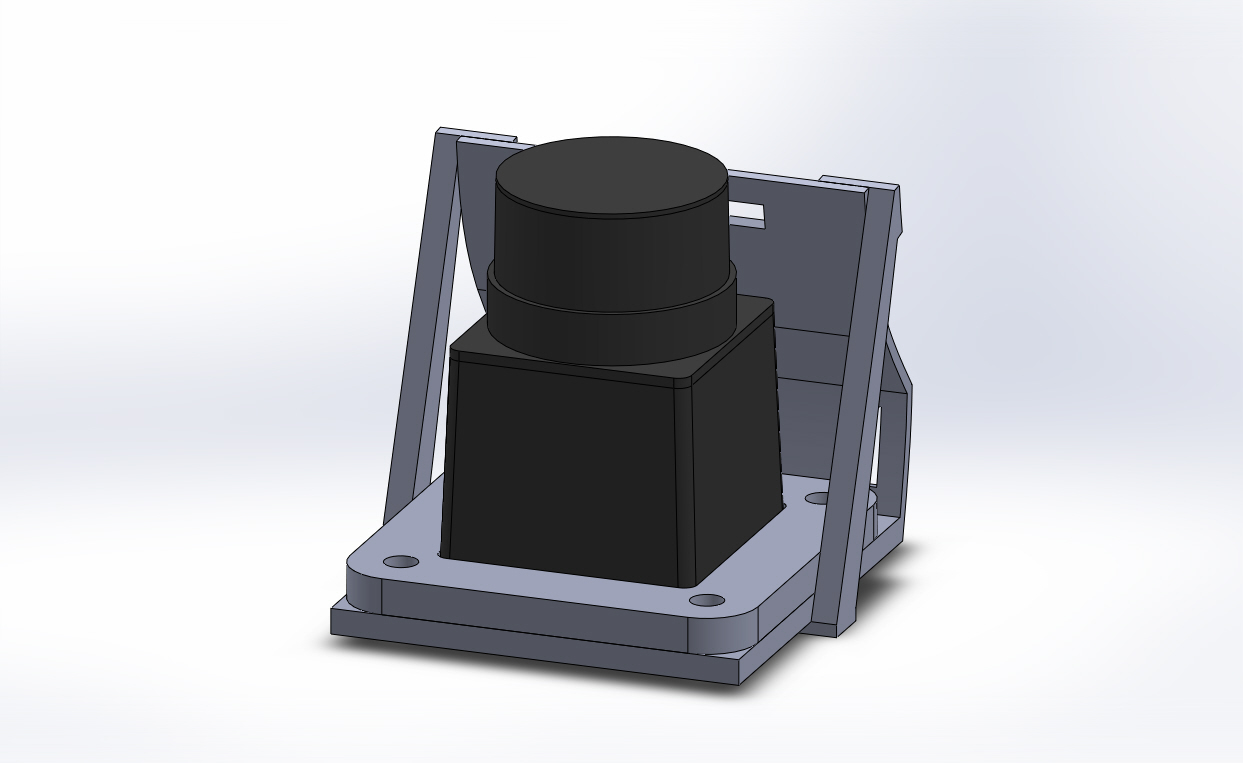
\includegraphics[height=0.4\textheight]{backpack/Assem_FrontOnly_Dimetric1.jpg}
  \caption{Figure showing assembled Nao Lidar.}
  \label{fig:nao_lidar_mount_dimetric1}
\end{figure}

\begin{figure}
  \centering
  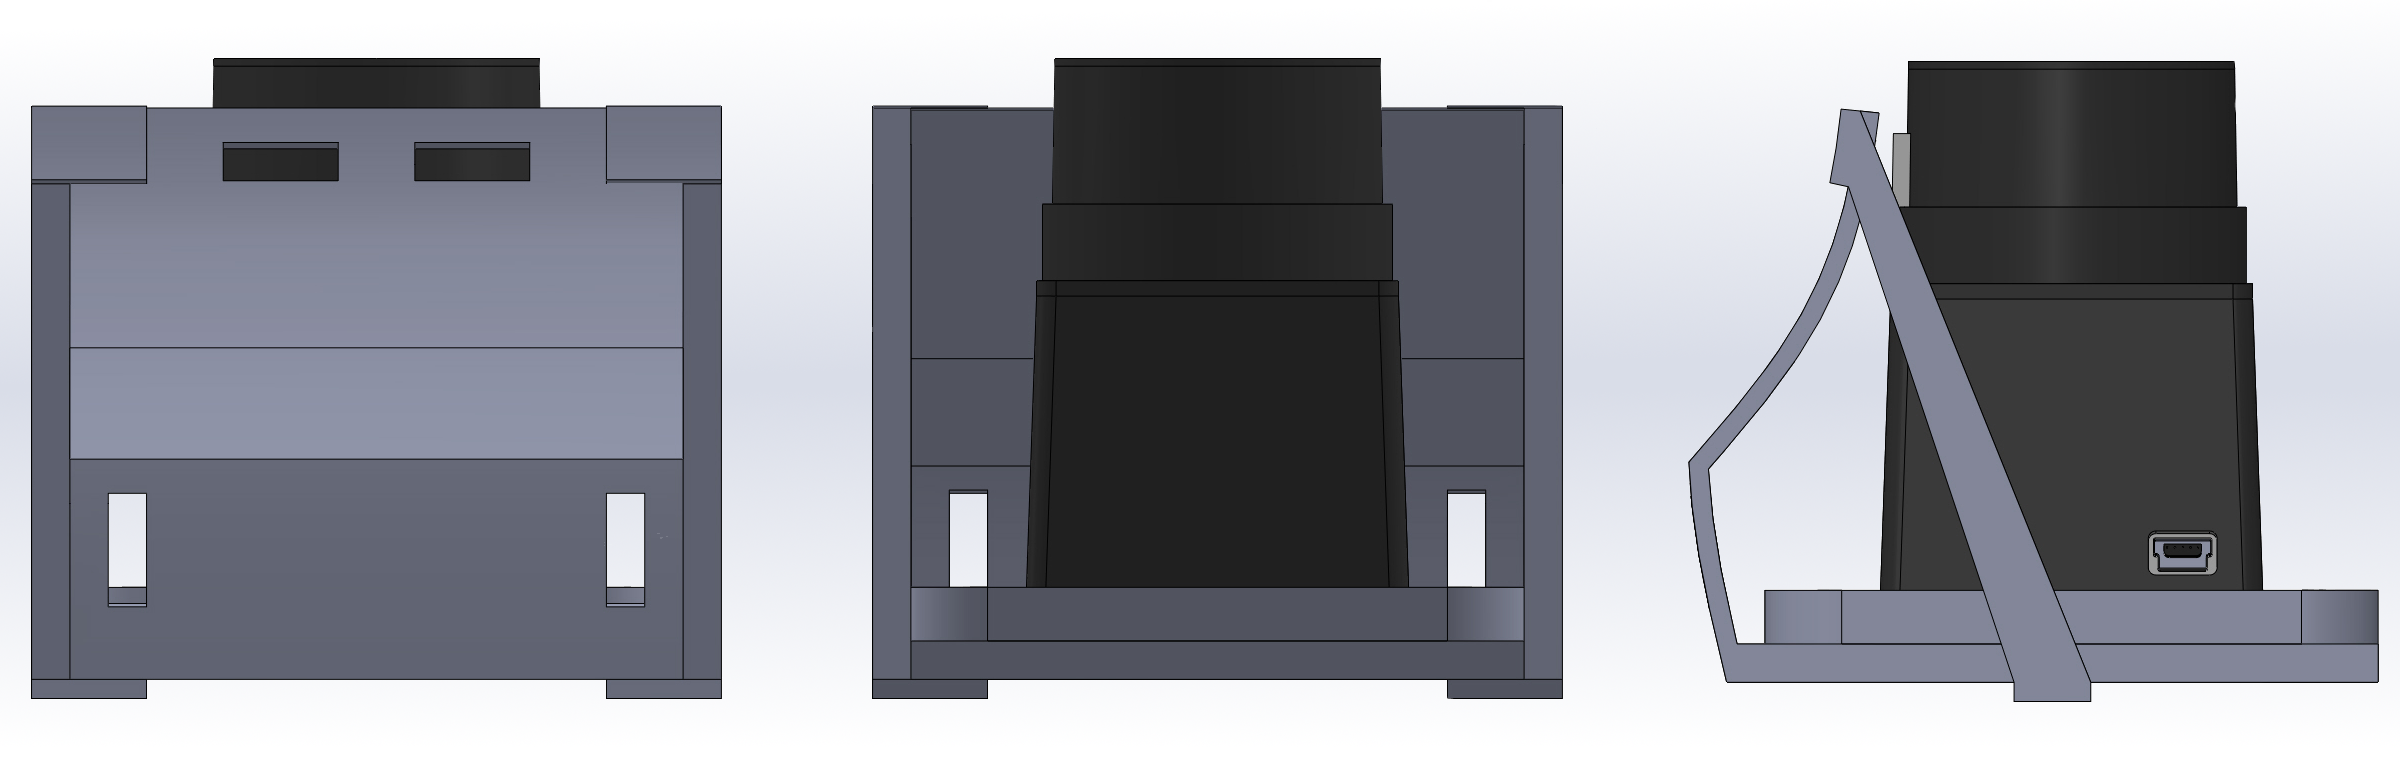
\includegraphics[width=\textwidth]{backpack/Assem_FrontOnly_Three_View1.png}
  \caption{Figure showing assembled Nao Lidar.}
  \label{fig:nao_lidar_mount_three_view1}
\end{figure}

\begin{figure}
  \centering
  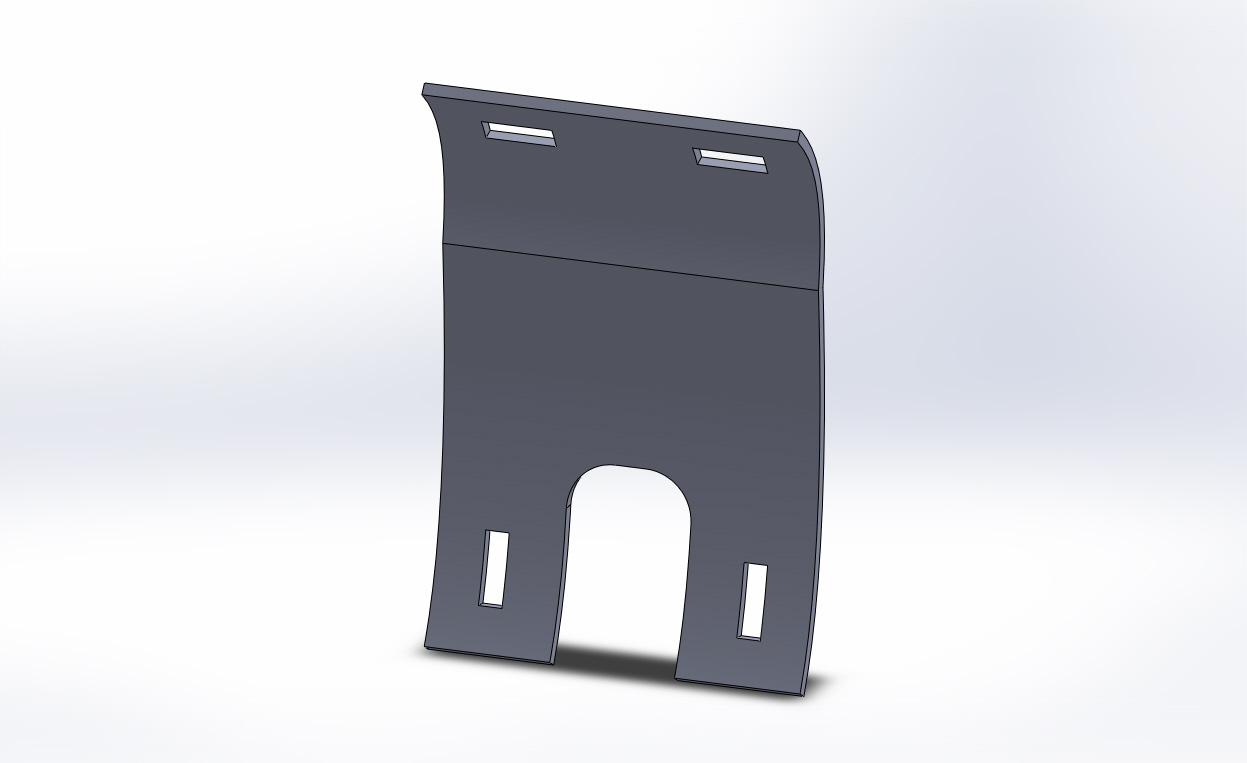
\includegraphics[height=0.4\textheight]{backpack/Back_Plate_Dimetric1.jpg}
  \caption{Figure showing assembled Nao Lidar.}
  \label{fig:nao_lidar_mount_backplate_dimetric1}
\end{figure}

\begin{figure}
  \centering
  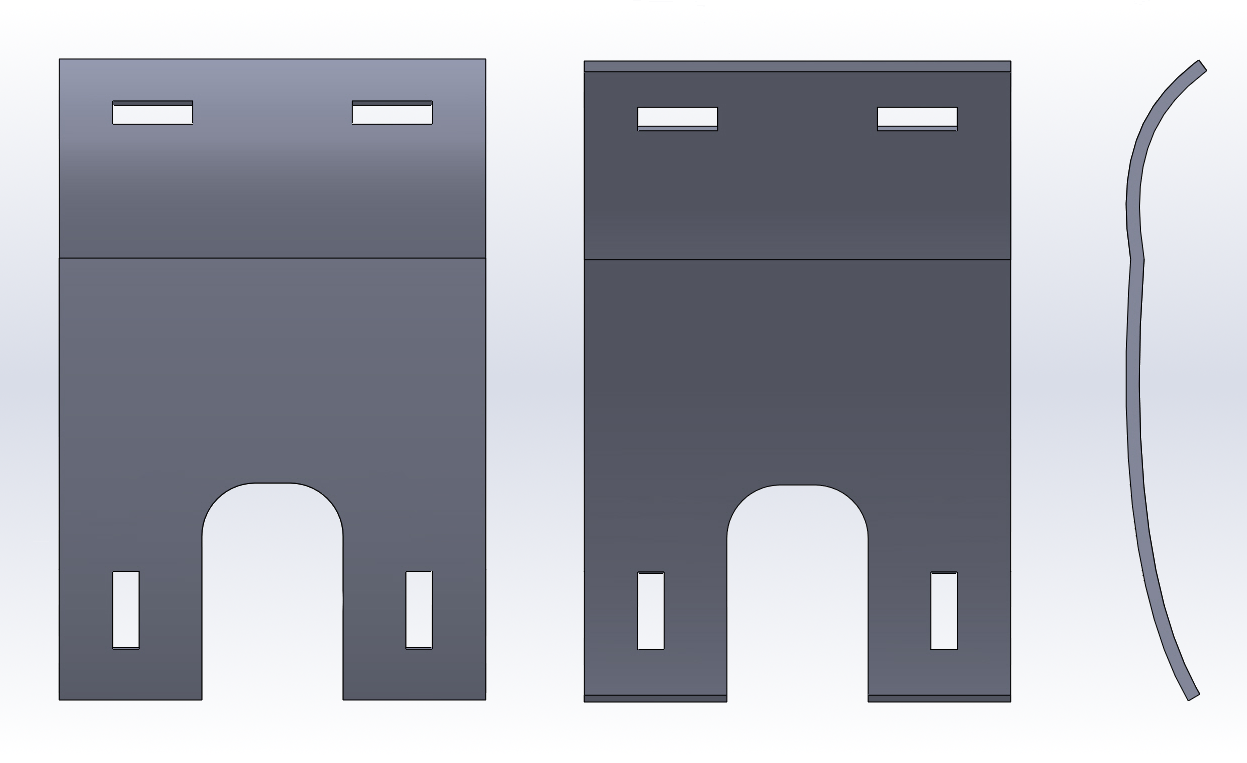
\includegraphics[width=\textwidth]{backpack/Back_Plate_Three_View1.png}
  \caption{Figure showing assembled Nao Lidar.}
  \label{fig:nao_lidar_mount_backplate_three_view1}
\end{figure}

\begin{figure}
  \centering
  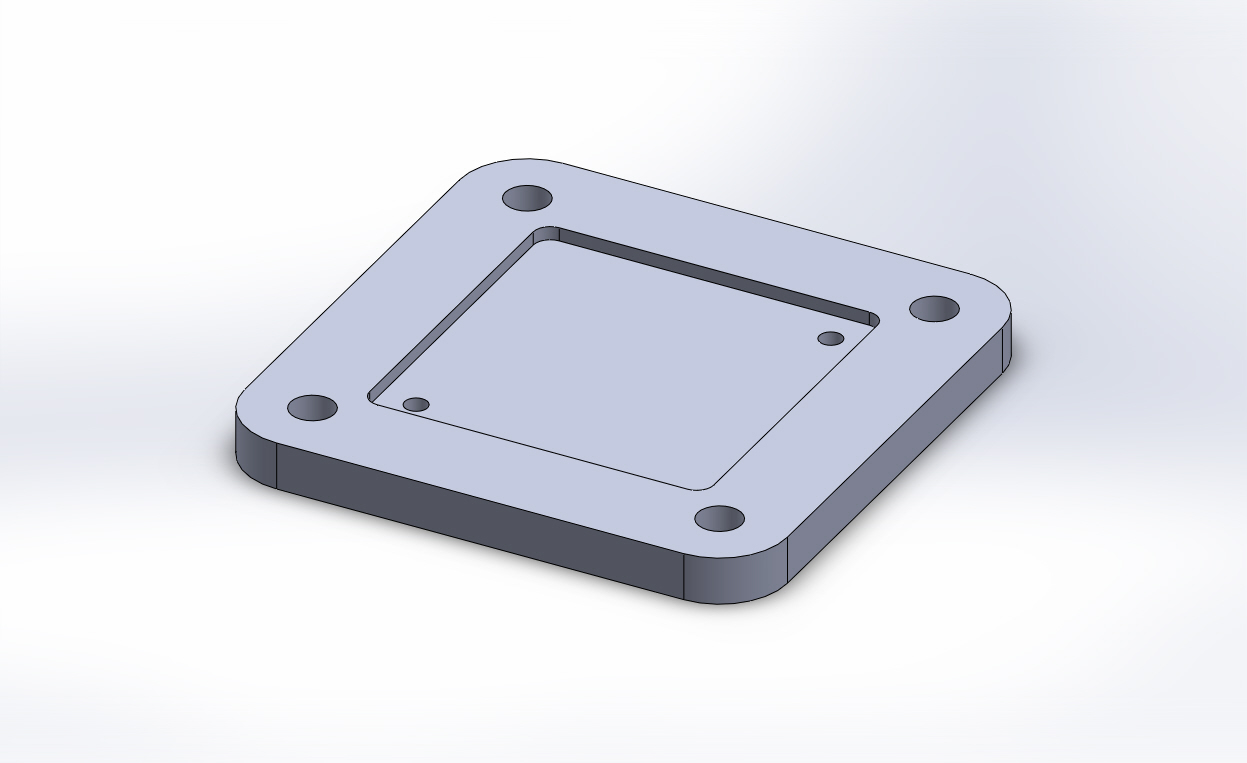
\includegraphics[height=0.4\textheight]{backpack/Base_Plate_Trimetric1.jpg}
  \caption{Figure showing assembled Nao Lidar.}
  \label{fig:nao_lidar_mount_baseplate_trimetric1}
\end{figure}

\begin{figure}
  \centering
  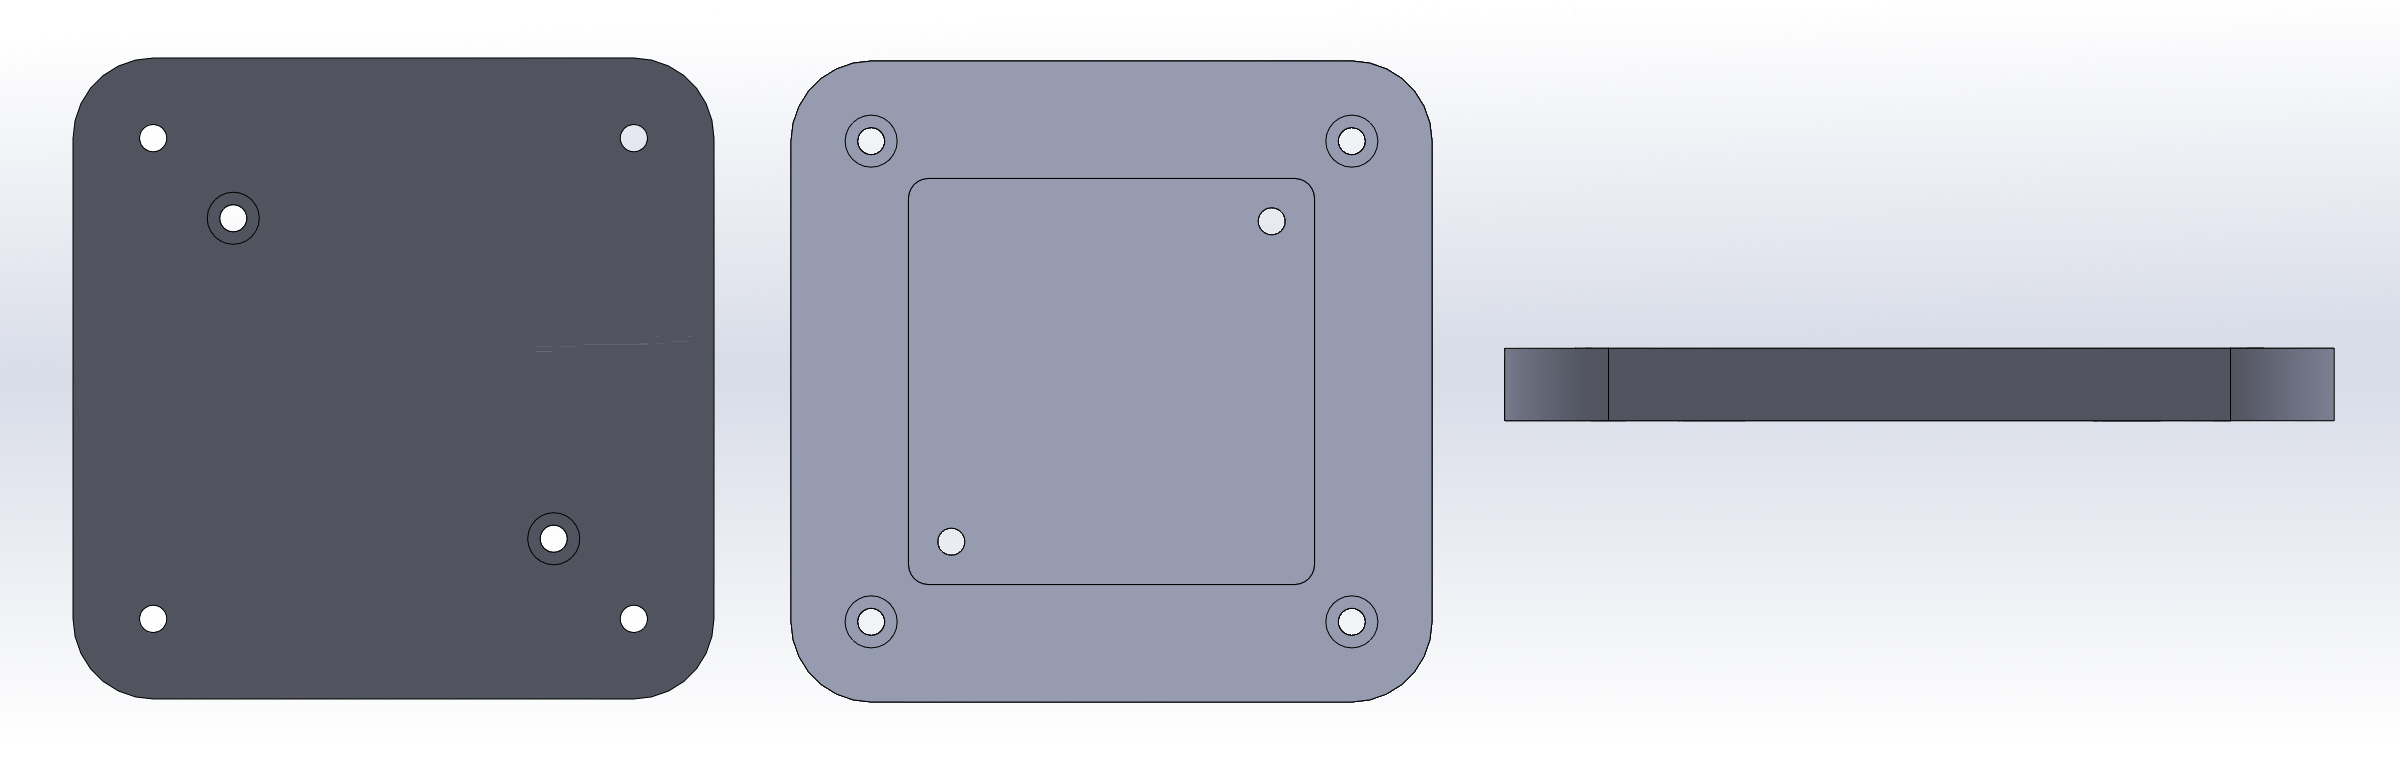
\includegraphics[width=\textwidth]{backpack/Base_Plate_Three_View1.png}
  \caption{Figure showing assembled Nao Lidar.}
  \label{fig:nao_lidar_mount_baseplate_three_view1}
\end{figure}

\begin{figure}
  \centering
  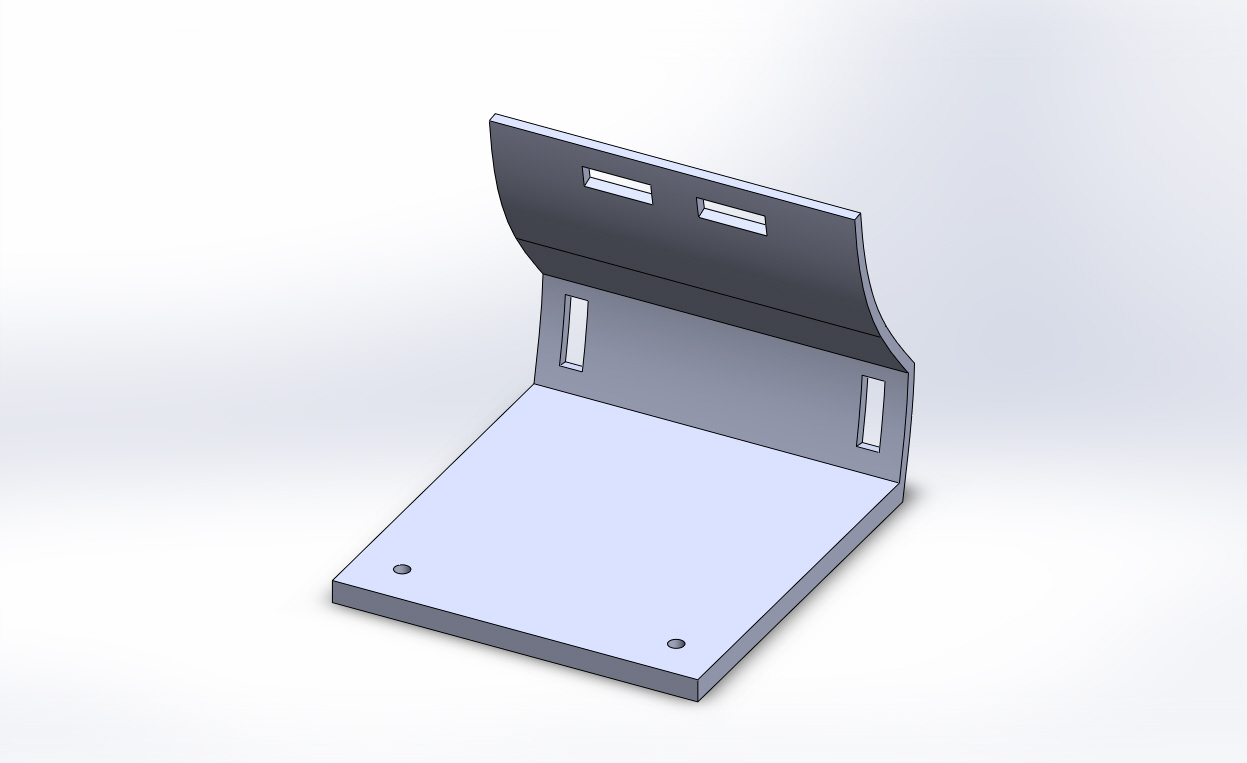
\includegraphics[height=0.4\textheight]{backpack/Front_Plate_Trimetric1.jpg}
  \caption{Figure showing assembled Nao Lidar.}
  \label{fig:nao_lidar_mount_frontplate_trimetric1}
\end{figure}

\begin{figure}
  \centering
  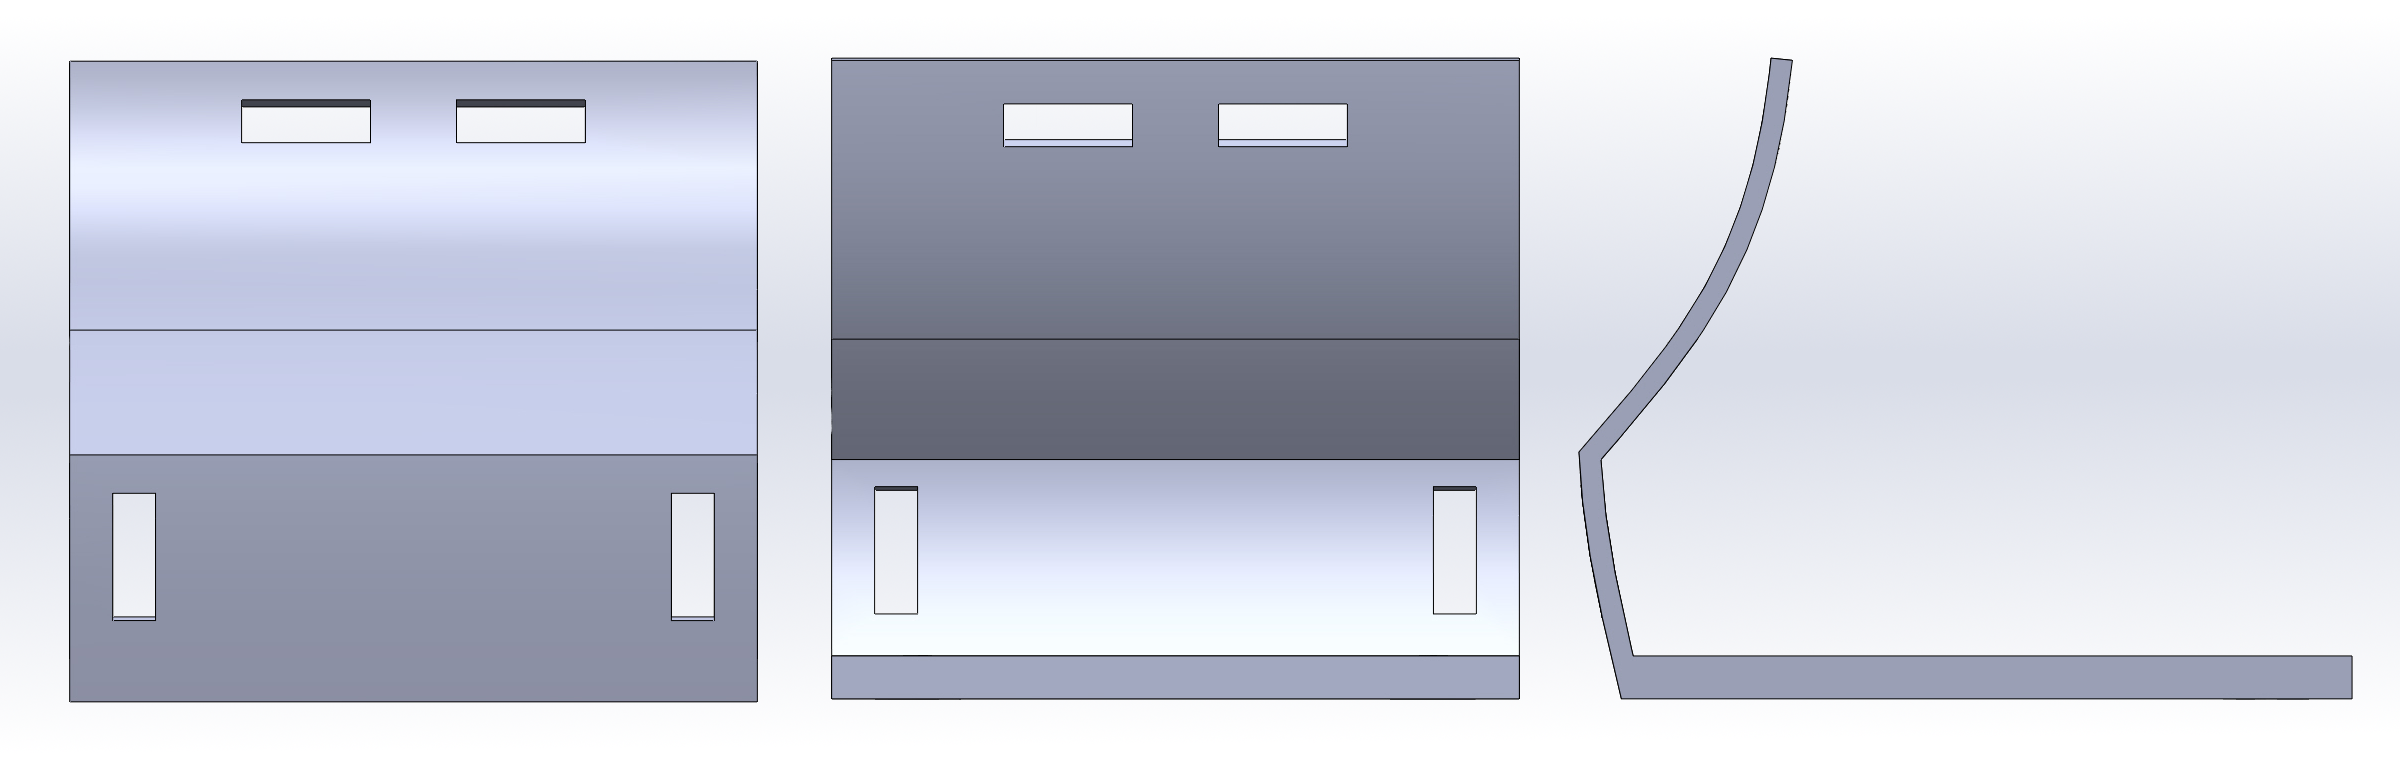
\includegraphics[width=\textwidth]{backpack/Front_Plate_Three_View1.png}
  \caption{Figure showing assembled Nao Lidar.}
  \label{fig:nao_lidar_mount_frontplate_three_view1}
\end{figure}

\begin{figure}
  \centering
  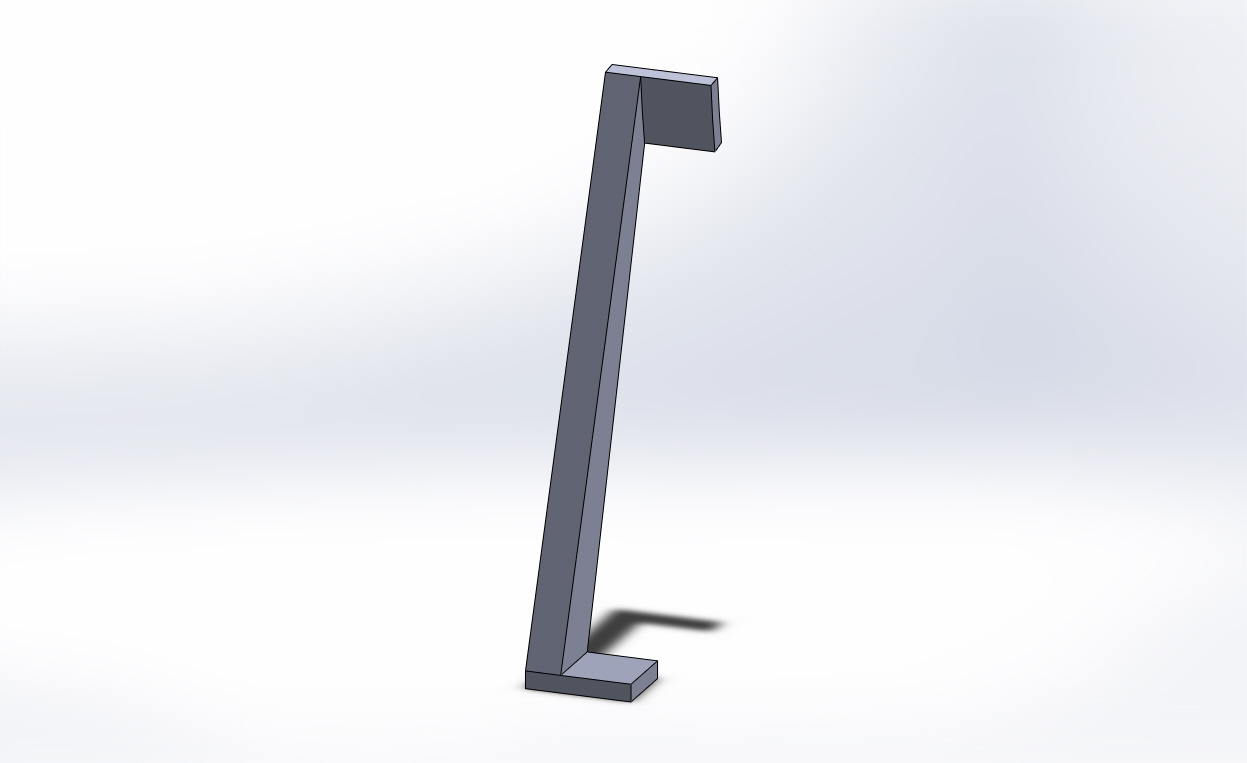
\includegraphics[height=0.4\textheight]{backpack/Support_Left_Trimetric1.jpg}
  \caption{Figure showing assembled Nao Lidar.}
  \label{fig:nao_lidar_mount_supportleft_trimetric1}
\end{figure}

\begin{figure}
  \centering
  
\includegraphics[height=0.4\textheight]{backpack/Support_Left_Three_View1.jpg}
  \caption{Figure showing assembled Nao Lidar.}
  \label{fig:nao_lidar_mount_supportleft_three_view1}
\end{figure}

\begin{figure}
  \centering
  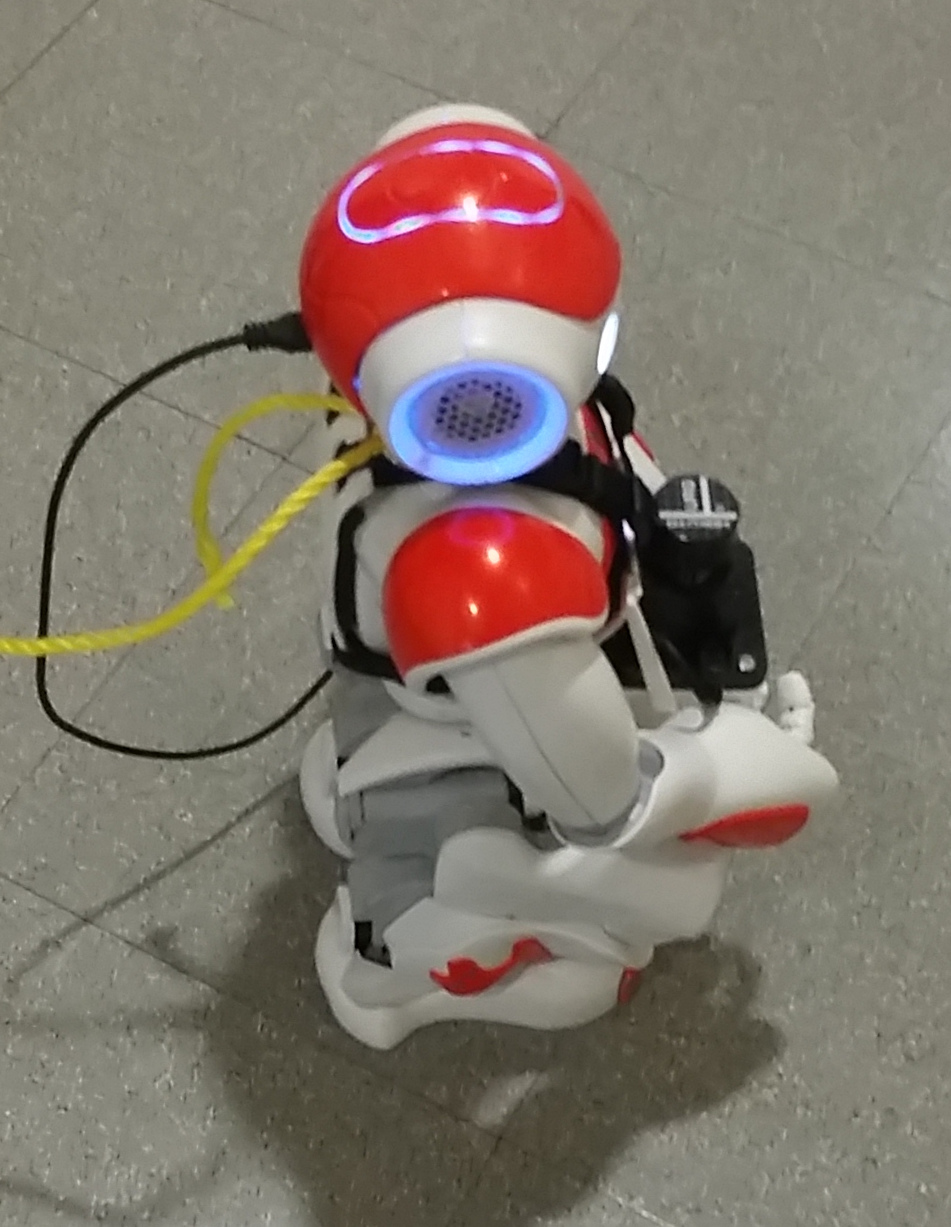
\includegraphics[height=0.4\textheight]{nao_with_mount2.jpg}
  \caption{Figure showing Nao with Lidar mounted to chest.}
  \label{fig:nao_lidar_mount1}
\end{figure}

\section{Software Framework}
So Nao comes with a much of good stuff. The API allows us to program in C++ or python and run locally or
remote. We can also test things quickly using Choreographe. Because it's linux we can also easily
run other non-aldebaran programs in python or using g++ complier.
The lidar runs on a python server, allowing the ground station and the Nao to easily see/use the data since
everything is over WiFi and the sockets don't care. How does this work?
How to log into Nao. Choreographe, remote run, and ssh for local run.

\subsection{NaoQi API and qibuild}
qibuild is what allows us to use the libraries remotely or locally without thinking. It's based on CMake
so you can add new libraries in just as you would with CMake on Linux.

The API is really a lot. You can command things on the joint level, nav level, pose level,
set velocities or positions, get orientation, distances, and joint angles or currents.
Everything is done with proxies.

% \subsection{Custom Library Framework}
\subsection{User Operation}
How do you start Nao, start Lidar? Log in to robot? Start program. Load program.
Start algorithms, stop them.

	
%%%%%%%%%%%%%%%%%%%%%%%%%%%%%%%%%%%%%%%%%%%%%%%%%%%%%%%%%%%%%%%%%%%%%%%%%%%%%%%%%%
%%% Navigation
%%% 
%%% Section 1 : Survey of Algorithms
%%% 	Subsection 1.1 : Classes of Algorithms
%%% Section 2 : Potential Fields
%%%	Section 3 : GODZILA
%%% mention that one aspect of navigation is vertically constrained spaces, connect to next chapter
%%%%%%%%%%%%%%%%%%%%%%%%%%%%%%%%%%%%%%%%%%%%%%%%%%%%%%%%%%%%%%%%%%%%%%%%%%%%%%%%%%
\chapter{Navigation} \label{ch:navigation}

%%% What is navigation? %%%
% Make this section less colloquial.
Navigation is the task of generating a series of commands that allow a robot to transit from its current pose
to some goal pose. This task encompasses a number of subtasks such as path planning, environment sensing, and obstacle
avoidance. As a robot transits through space from its current to goal pose, it necessarily visits a series
of intermediate poses the choice of which depends on its kinematic constraints and the constraints of the environment it transits through. 
Collectively, this set of poses as a time sequence is known as a path. 
The spacial region in which the robot operates is known as the task space and all kinematically feasible configurations is known as the
configuration space.  Typically, the environment a robot traverses is not free space but also contains obstacles 
which constrain the paths which can be taken to the goal. While in some 
controlled environments the location of obstacles can be known \textit{a priori} and supplied to the robot in the form of a map, often the
robot will have the task of creating a map which describes the location of these obstacles. In some situations, ``global" 
sensors can view the entire environment within which the robot will operate and can capture all of the constraints while in others (especially
in the case of mobile robots) only ``local" sensors mounted to the robot are available to detect environmental limitations
to the robot's path as they are encountered. Even more challenging is the case where the environmental obstacles are not
static but are moving adding a time varying element to the obstacle avoidance problem.

% In the first place that you mention the categories, you can clarify that the categories are not mutually exclusive,
% but that algorithms are classified into combinations of categories.

% Algorithms that solve the navigation problem are sometimes described according to four major categories.

% Here's one way to split up things:
Algorithms that solve the navigation problem are sometimes described according to four major categories (though there are many
other categories with which these algorithms could be described with). These categories are not mutually exclusive, and algorithms
are commonly attributed with multiple classifications.
The first two, known as global or local, speak to the amount
of spatial data or time horizon considered when planning a solution. If only a short time horizon or occlusions in the immediate
spatial region are accounted for, then the algorithm is considered local, otherwise it is thought of as global.
The other two deal with how the spaces or paths are represented, continuously or discretely. If the algorithm breaks
up these spaces into finite resolution pieces, then it is discrete. Continuous algorithms choose some sort of parameterization
to the spatial or environmental constraints using a model. Often algorithms are some mixture of all of these four categories.

The algorithm used for navigation in this thesis is the GODZILA navigation algorithm, 
which can be categorized as a local continuous algorithm based on the potential fields navigation strategy. 
While in many environments GODZILA solves the navigation problem, it can also be used in conjunction with global algorithms
that can plan way points to the goal without having to consider the detailed local environment.

%%% Addendum's %%%
In the design on the obstacle avoidance algorithm for a robot, it is important to consider how different local sensors 
can affect the choice of navigation algorithm. The Nao humanoid platform
used in this thesis is equipped with two sonar sensors for obstacle detection. Details on these are given in Chapter \ref{ch:platform}.
These sensors have a broad angular range and cannot provide information about where within this cone obstacles are located.
This enables the robot to avoid colliding with objects directly in front of it but might cause the obstacle avoidance algorithm
to preclude the discovery of possible paths (e.g., narrow corridors between obstacles).
Conversely, scanning laser rangefinders (such as the one mounted to the Nao and described in Chapter \ref{ch:platform}) have a
very high degree of angular resolution and provide hundreds of range measurements. This allows for a more accurate description
of environmental occlusions allowing more paths to be considered for traversal.
% [Insert picture of sonar cones vs lasers.]
\begin{figure}
	\centering
	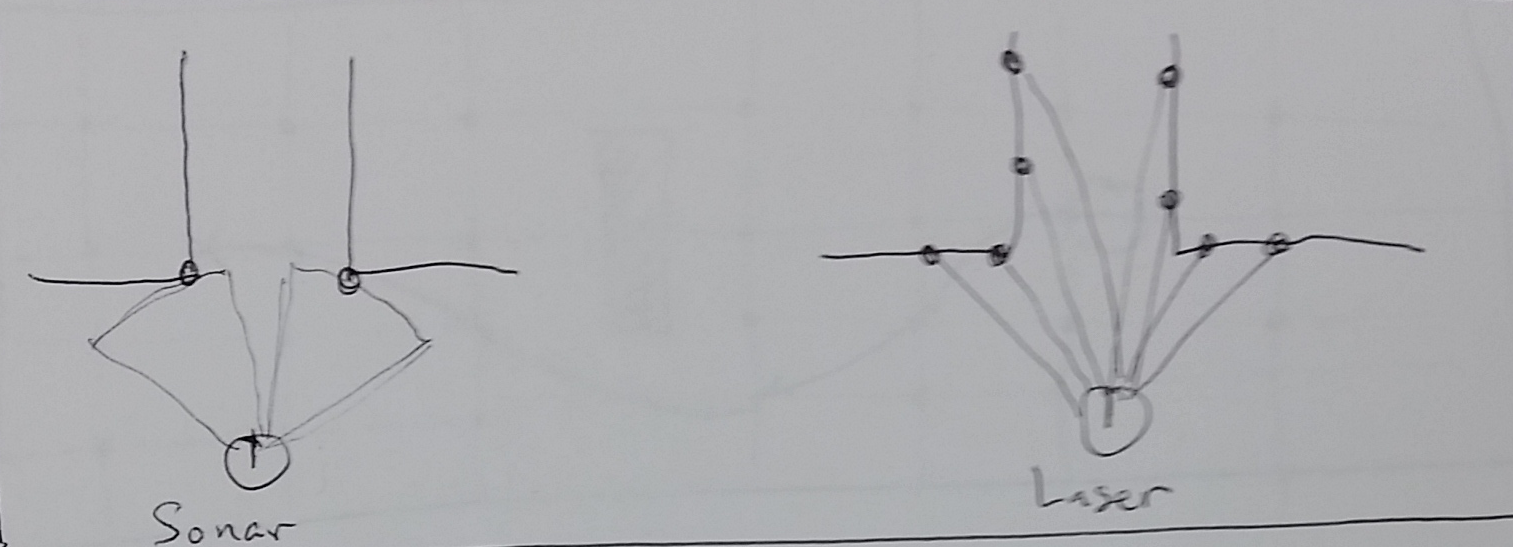
\includegraphics[width=\textwidth]{sonar_lidar_rough1.png}
	\caption
	{Sonar sensors are typically preferred when needing to detect the presence of an obstacle without
	 needing precise position information. The location of a chair leg in the path of a robot would be
	 detected by sonar while not knowing its position in the sonar cone. Laser rangefinders have very
	 narrow beam width, typically requiring many of them to be effective at describing an environment.
	 If many measurements are available at high angular resolution, then they can be very effective at
	 describing the width of narrow apertures.}
	\label{fig:sonar_vs_lidar1}
\end{figure}

The notion of what objects in the environment occlude a path and which do not can be viewed as a function of the gait 
(or mode of locomotion) used by the robot. If the robot is restricted to a plane, such as the case in many ground vehicles,
then an object of similar size to the vehicle could prevent traversal through that position. If the robot can also fly then
that object may not present an impediment to proceeding towards the goal.
While still not transiting through that exact position in 3D space, the 2D projection of the path onto
the plane will appear to have moved through the obstacle. This can be though of in terms of a transformation of the obstacle set according to the different
motion modalities, making a 2D planner still applicable to the problem. In Chapter \ref{ch:crawl_gait},
a crawling gait for the Nao robot is considered which allows it to go under occlusions that it would otherwise need to plan
around.


\section{Algorithm Classifications}
Here some of the different notions common to navigation algorithms are explored. These classifications are sometimes useful
for the navigation engineer to think about as tools available to solve the navigation problem. While additional classifications
and subclassifications of algorithms can be considered, the following description is intended as a brief overview of the 
essential concepts.

\subsection{Global}
One approach to the navigation problem is to consider the entire task and configuration space of a problem when generating
a solution. For example, the task space of a robot arm might be the pose of the end effector and all of the occlusions
within that space. The configuration space would be the set of all valid joint angles that the arm can attain. Using this,
an algorithm can compute a time sequence of poses or movement commands that the robot should execute in order to bring it
from its current pose to the final pose. While this approach is ideal in the sense of generating a solution to the 
original problem, it has several practical disadvantages. One requirement of the algorithm is having a complete description 
of the task space. In many cases global knowledge of occlusions while planning is not available meaning that when new
obstructions are observed, the algorithm needs to replan the path. The other commonly encountered problem with these
algorithms is when the magnitude of the space to be planned through is so large that computing a solution cannot be done
in real-time.
% [Insert picture of global path and local directions.]
\begin{figure}
	\centering
	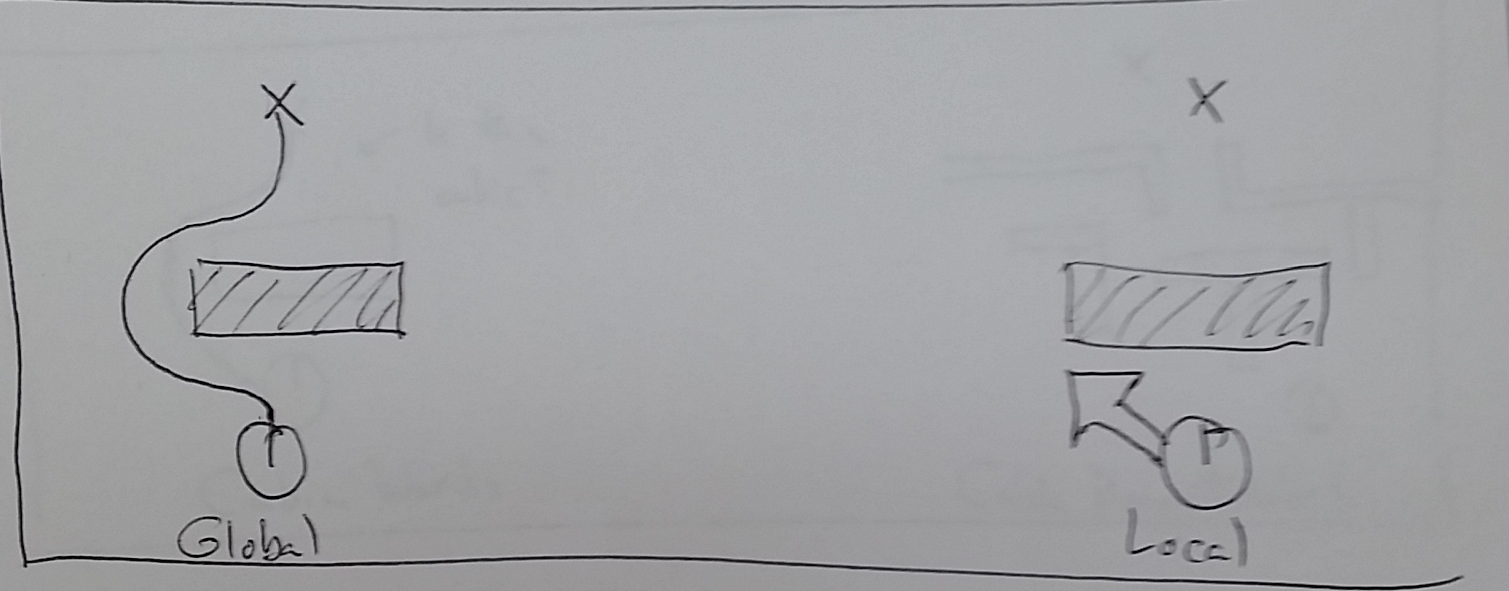
\includegraphics[width=\textwidth]{global_local_rough1.png}
	\caption
	{In global approaches, an entire path is planned to the goal before commanding the robot. In local 
	schemes, the robot is given commands calculated as a function of its position and the local environment and
	a complete path to the goal is typically precomputed. }
	\label{fig:global_vs_local1}
\end{figure}

\subsection{Local}
A different approach to the navigation problem is generating commands based only on the current information available 
or a short history about the environment. In the robot arm example, there might be a sensor such as a camera that
can detect objects that are obstructing the end effector from reaching the goal and instructs the arm to move around it.
Such algorithms usually have the advantage of being quick to compute as compared to their global counterparts because
they only have to consider a small subset of the task and configuration space. Their main disadvantage is that since they
only use such a limited amount of information, they can become trapped in local optima that do not allow the robot 
to achieve the desired pose.

%%% Continuous and Discrete %%%
\subsection{Discrete}
Orthogonal to the ideas of local and global path planning which deal with the scope of the time and space being considered
when generating navigation commands is how these spaces are represented. One way to represent the space is to break it
up into a set of discrete locations and then plan through that discretized representation. The task space for example could be divided into uniform 
spatial regions which an algorithm can consider visiting when planning a path. Alternatively, as with the robot arm example,
a finite set of movement commands can be considered and iterated through while generating a solution. 
Graph-based search algorithms such as  Dijkstra's algorithm or A* are examples of discrete solvers.
An advantage to this is that paths with complex shapes can be generated to accommodate difficult constraints. 
One point however to consider in this approach is how finely to resolve the task or configuration spaces. 
Coarser discretization can allow a solution to be computed rapidly but might miss more optimal solutions. 
% [Insert grid based path example.]
\begin{figure}
	\centering
	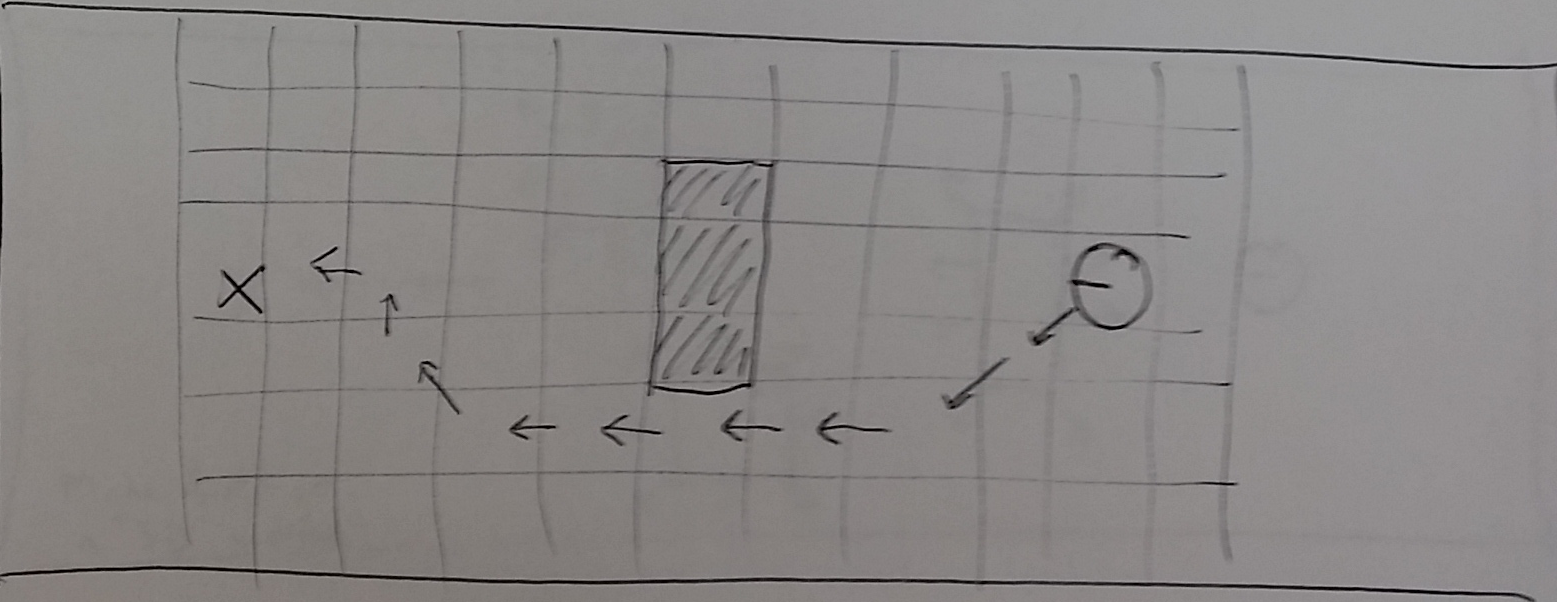
\includegraphics[width=\textwidth]{grid_world_rough1.png}
	\caption
	{The environment here is being represented as occlusions in a discrete grid of locations.
	This allows the robot to plan through successive locations to the goal using graph-based techniques.}
	\label{fig:grid_world1}
\end{figure}

\subsection{Continuous}
Continuous spatial representation avoids the problem of having to choose a discretization resolution. The movement commands or paths
are planned in a continuum allowing paths to take on intermediate values not available at a given discrete resolution.
Continuous representation instead has a different problem of paths needing to take on particular solution forms. A path
through the task space might be represented as a cubic spline from the current pose to the goal pose. This path has access
to the entire task space but may not be able to construct a path under complicated environments with many obstacles. Often
instead of using a single cubic, designers will use a series of cubics, the termination of one being the starting
position of the next, until the goal is reached. 
Alternatively, instead of restricting the path representation to a series of cubics, other trajectory forms can be
utilized as a library of representations such as higher-order polynomials, trigonometric functions, etc.
One example of such a planner is known as a ``maneuver-based" planner.
% [Insert figure than shows a successful cubic spline path and a maze where you couldn't use that.]  
\begin{figure}
	\centering
	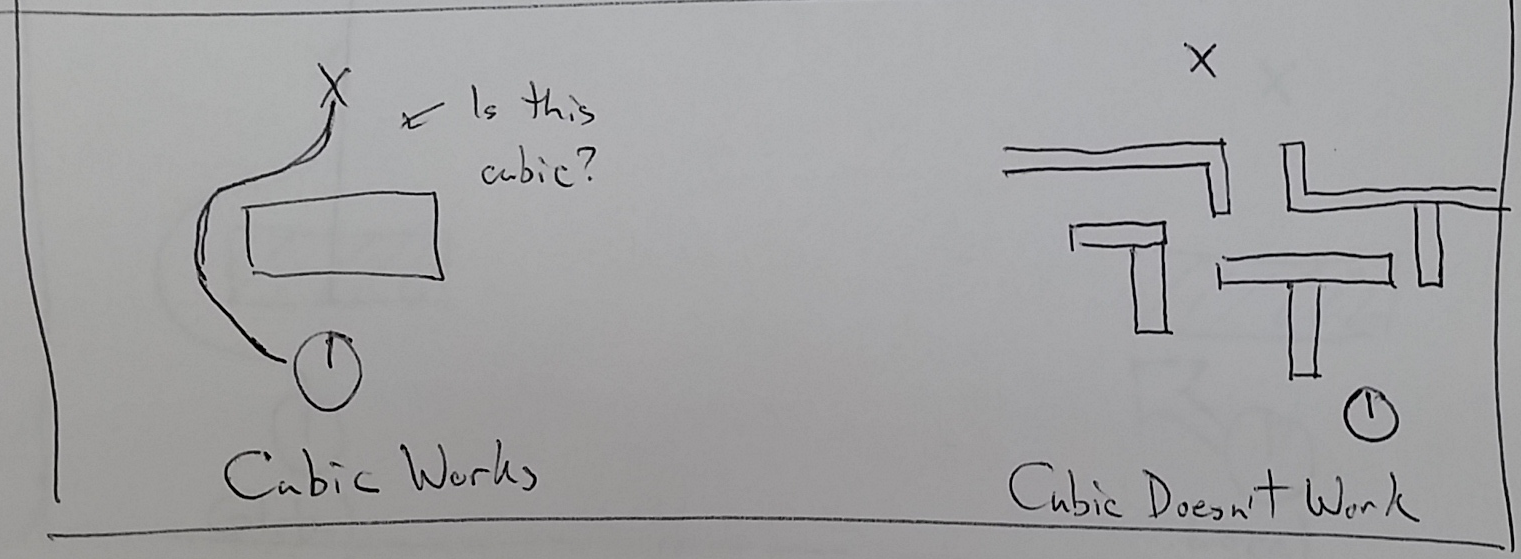
\includegraphics[width=\textwidth]{cubic_rough1.png}
	\caption
	{This figure shows two sample environments. On the left, the robot can follow a trajectory that takes
	a cubic form and reaches the goal location. On the right, a more complicated environment is shown where a single 
	cubic cannot describe an appropriate path.}
	\label{fig:cubic1}
\end{figure}

\subsection{Composite Approaches}
In order to combine the strengths and combat the weaknesses, the above approaches are often combined to form a more robust
navigation solution. Global plans can be generated as a series of intermediate goals or way points for local planners to 
navigate towards. These way points can be planned on a coarse discrete grid that is quick to compute while low dimensional
continuous trajectories are plotted between them. Lattice planners are an example of such a composite algorithm. 
% [Show lattice plan figure.]
\begin{figure}
	\centering
	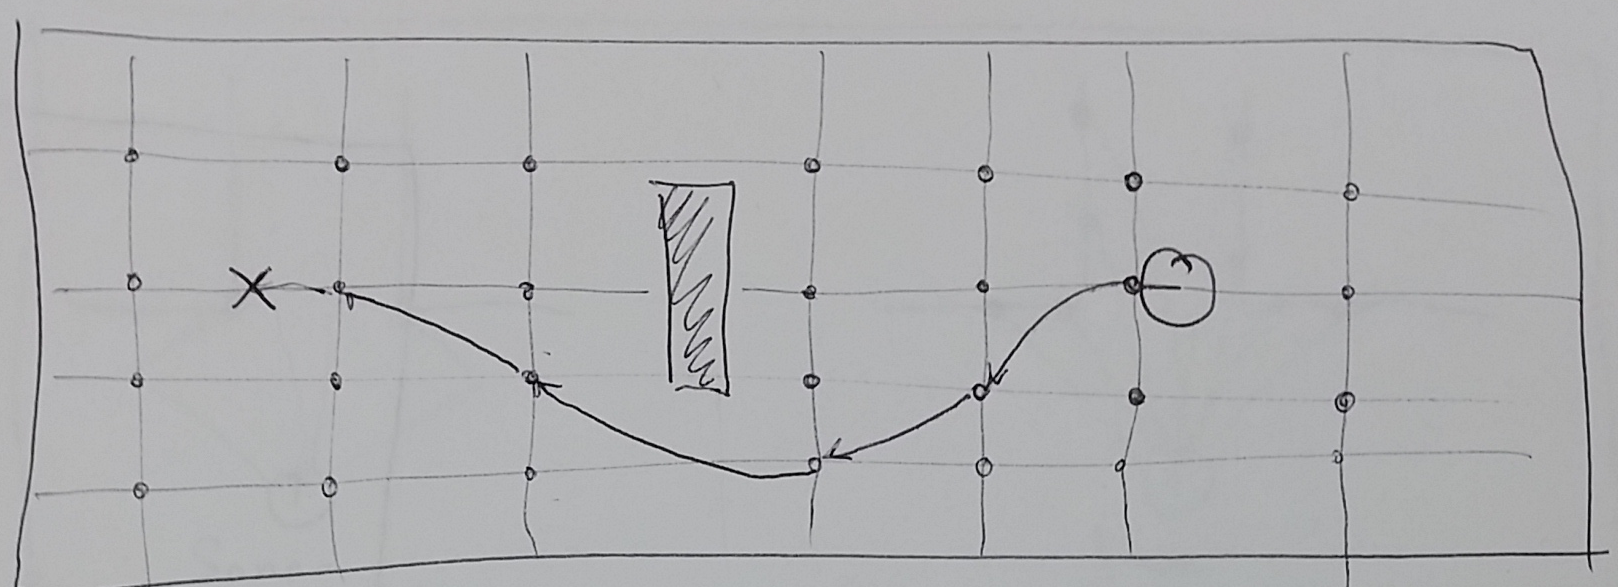
\includegraphics[width=\textwidth]{lattice_rough1.png}
	\caption
	{A lattice planner is an example of a composite discrete and continuous path planner. The planner
	first plans through a discrete grid and then designs trajectories that bring the robot from each point in the planned discrete grid to the next.}
	\label{fig:lattice1}
\end{figure}

\section{Potential Fields} \label{sec:navpotfields}
Potential fields algorithms are continuous local planners. They work on the concept of modeling the robot as a sort of
charged particle (like an electron) and obstacles in the environment are modeled as having the same polarity of charge as the robot thereby producing a repulsive field pushing the robot away
from them. The goal location in is modeled as having an opposite charge to the robot and thus produces an attractive force, pulling the robot towards it. As the robot moves through
the environment, it detects objects and generates motion commands based on its range and direction. 
\begin{figure}
	\centering
	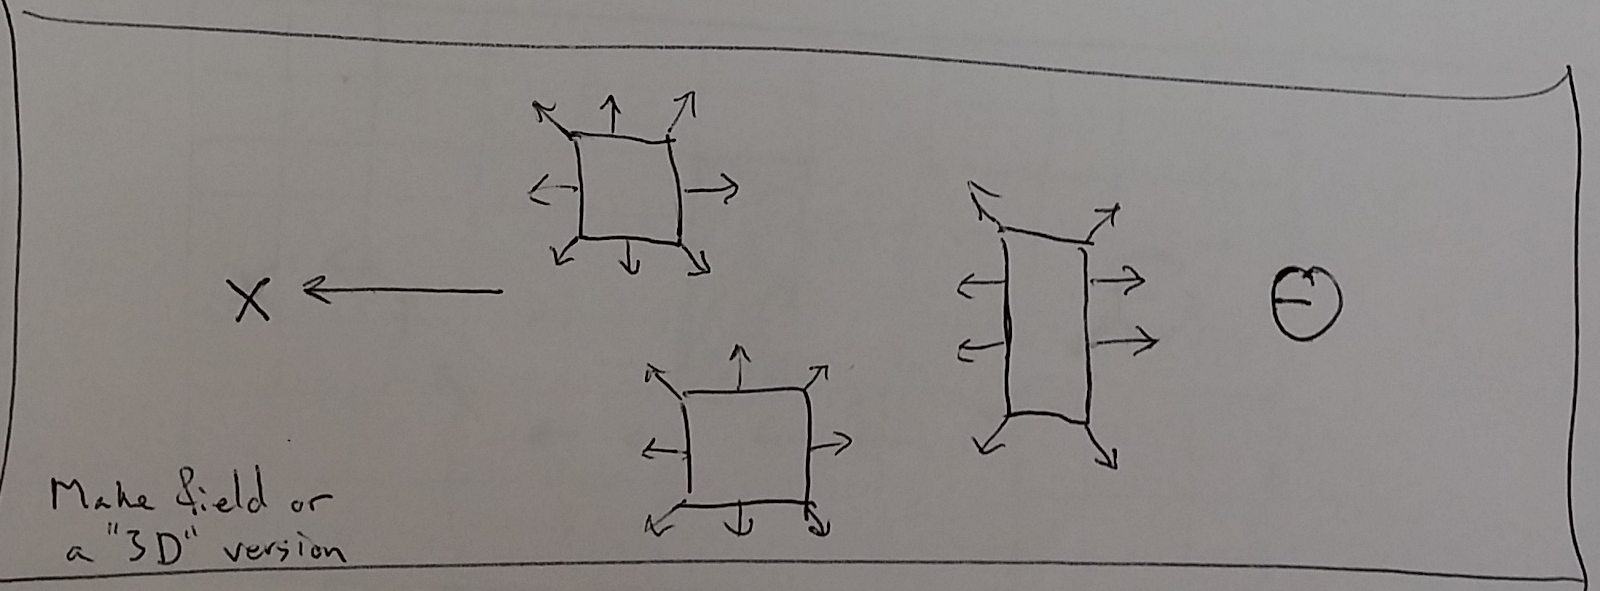
\includegraphics[width=\textwidth]{potentials_rough1.png}
	\caption
	{Visualization of potential fields idea. Objects in the environment emit a field that repels the robot
	 and the goal emits an attractive field. This can be visualized as a 2D or 3D vector field.}
	\label{fig:potentials1}
\end{figure}

Given a vector $x_r$ which describes the position of the robot in the task space and the positions of obstacles
$m_i$ in the set of all obstacles $M$, a force vector $f_i$ can be generated for each obstacle that describes the 
magnitude and direction of the repulsive force applied to the robot by the obstacle. The force direction
is in the opposite direction of the relative bearing of the obstacle to the robot with magnitude being inversely
proportional to the distance of the obstacle from the robot. Equation \ref{eq:potentials_eq1} shows an example
of force vector generation.

\begin{align}
	\norm{f_i}  &= \frac{-c_i}{\norm{m_i - x_r}^\alpha}\\
	\angle{f_i} &= \angle(m_i - x_r)
\label{eq:potentials_eq1}
\end{align}

$m_i - x_r$ is the location of the obstacle relative to the robot and $c_i$ is a positive scalar used to tune force
magnitude. In some implementations, $c_i$ can be a function of the relative bearing, for example, decreasing the repulsion
effect if the obstacle is not in the direction of the goal. The parameter $\alpha$ in general can be any positive scalar
but is often picked to be 2.

For the goal seeking behavior, the equations are similar, with the direction of the force being in the direction of the 
goal, rather than away from it.

\begin{align}
	\norm{f_g}  &= \frac{c_g}{\norm{x_g - x_r}^\gamma}\\
	\angle{f_g} &= \angle(x_g - x_r)
\label{eq:potentials_eq2}
\end{align}

$x_g - x_r$ in equation \ref{eq:potentials_eq2} is the relative location of the goal with respect to the robot and $c_g$ is some positive
tuning scalar. $\gamma$ is some positive scalar, typically 2.

The sum of these forces is used to produce a force vector $f_r$ used to command the robot away from obstacles and towards the goal
location. 

\begin{equation}
	f_r = f_g + \sum_{i = 1}^{\norm{M}} f_i
\label{eq:potentials_eq3}
\end{equation}

where $\norm{M}$ is the number of obstacles (modeled as a discrete set).

\section{GODZILA} \label{sec:navgodzila}

GODZILA (Game-theoretic Optimal Deformable Zone with Inertia and Local Approach) \cite{Krishnamurthy07} is a local 
continuous navigation algorithm based on the potential fields idea. In contrast to some potential fields formulations
which work on the range and bearing of objects in the environment, GODZILA uses the sensor information about occlusion
locations directly in order to formulate navigation commands. It is a memoryless algorithm and does not attempt to
build a map of the environment making it very lightweight in terms of both computation and memory. It can be implemented
on a variety of vehicles and is suited for the cases where a low computational power microcontroller is utilized.
It has three components which are an optimization cost, a straight line planner, and a stochastic local minima escape strategy.

Figure \ref{fig:godzila_setup1} illustrates the key variables in the formulation.
\begin{figure}
	\centering
	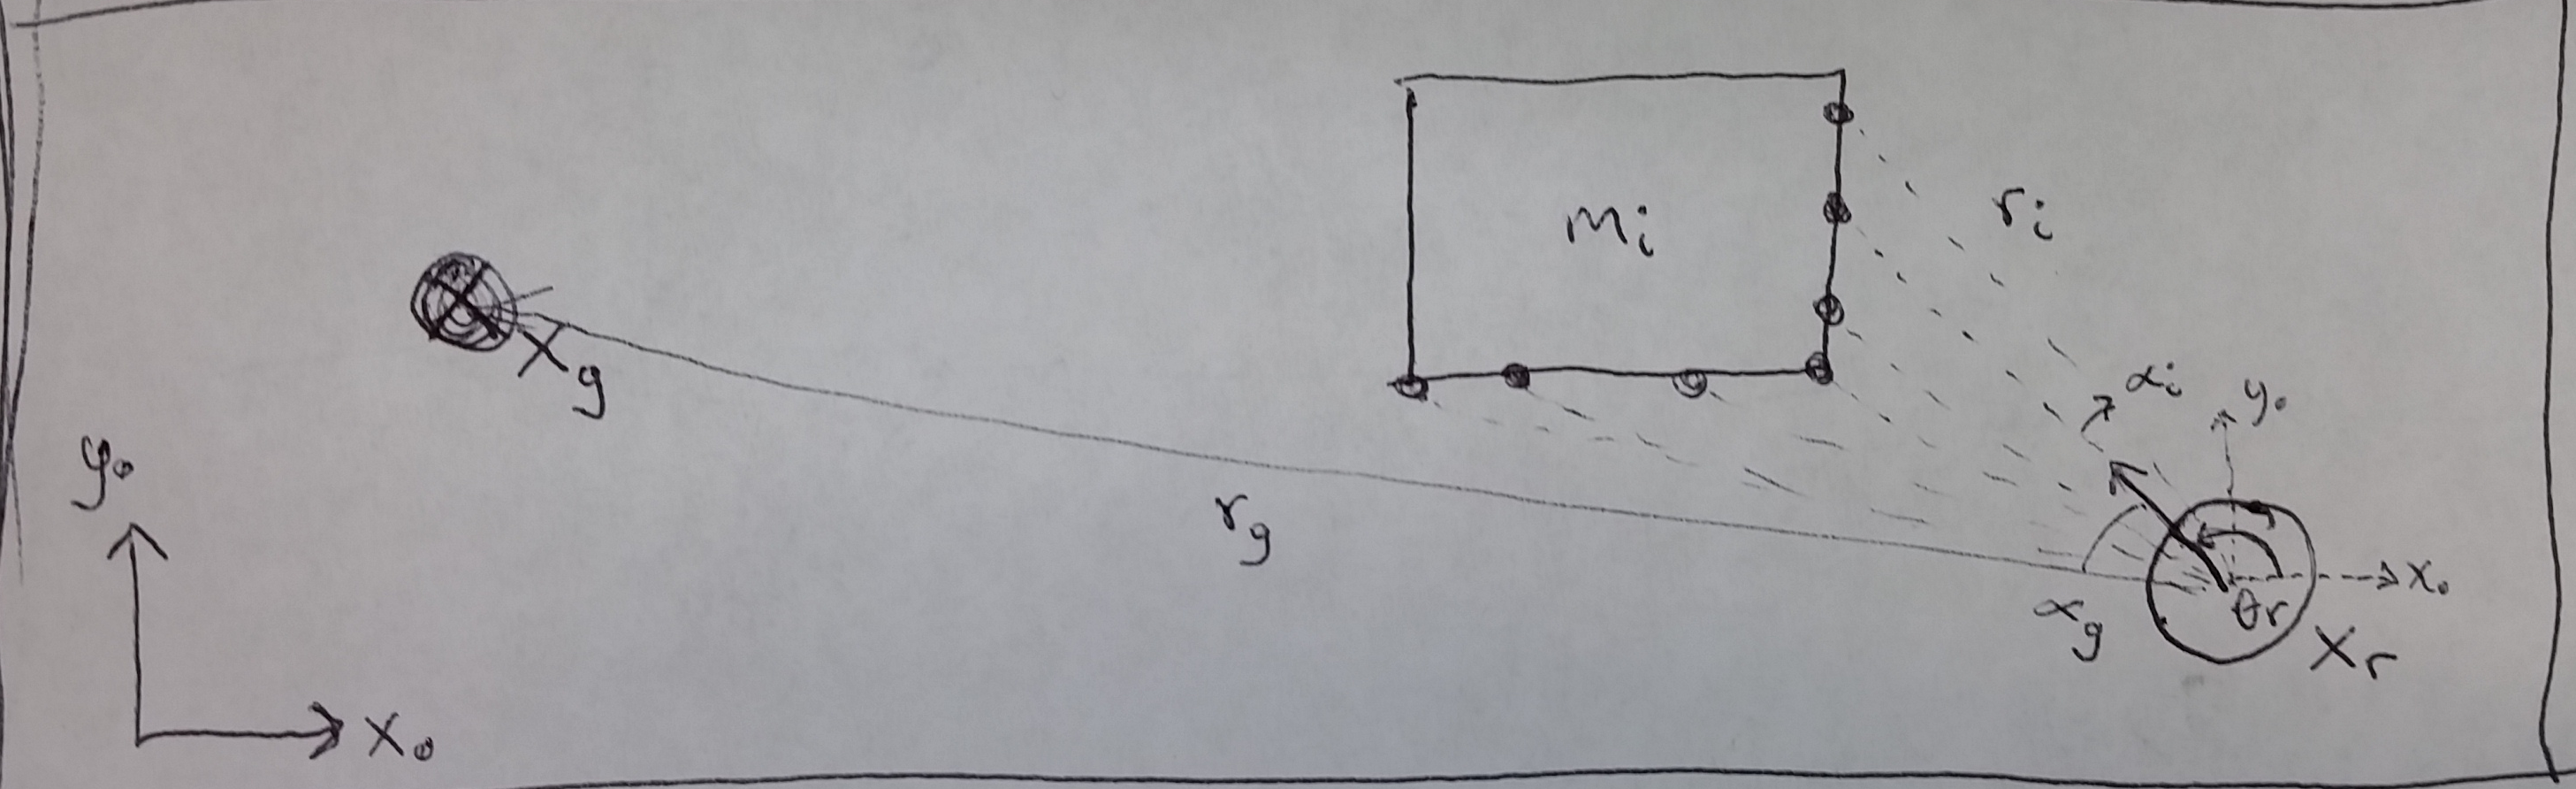
\includegraphics[width=\textwidth]{godzila_rough1.png}
	\caption
	{Illustration of various variables utilized in GODZILA. Range and bearing of the goal relative to the robot are required
	 as well as being able to take range measurements to occlusions and knowing the relative bearings of these measurements.}
	\label{fig:godzila_setup1}
\end{figure}

Taking a 2D example of the application of the GODZILA algorithm, we have the following terms:

\begin{description}
	\item[$x_0$] is the x-axis of the inertial frame.
	\item[$y_0$] is the y-axis of the inertial frame.
	\item[$x_r$] is the (x,y) location of the robot in the inertial frame.
	\item[$\alpha_r^\prime$] is the new heading the robot should be commanded to in the robot frame.
	\item[$x_g$] is the (x,y) location of the goal in the inertial frame.
	\item[$r_g$] is the range to the goal relative to the position of the robot.
	\item[$\alpha_g$] is the bearing to the goal location relative to the orientation of the robot.
	\item[$z_i$] is the $i^{th}$ sensor measurement made by the robot which includes range and bearing to an occlusion.
	\item[$r_i$] is the $i^{th}$ range measurement to an occlusion relative to the position of the robot.
	\item[$\alpha_i$] is the bearing angle to the $i^{th}$ sensor measurement.
\end{description}

In this formulation, it is assumed that there is some mechanism to allow the robot to get an estimate of the relative
range and bearing to the goal location $r_g$ and $\alpha_g$ and that the robot has some sensors that can provide range
and bearing to occlusions in the environment.

\subsection{Optimization Formulation} \label{subsec:navoptimization}
The formulation of the GODZILA algorithm is in terms of an optimization cost. The goal of the algorithm is to bring the robot
towards the goal while preventing it from colliding with obstacles. With this intuition the cost function has three components:

\begin{enumerate}
	\item $J_1(\alpha_r^\prime)$ which rewards goal seeking by penalizing directions other than those towards the goal.
	\item $J_2(\alpha_r^\prime)$ which penalizes directions towards occlusions.
	\item $J_3(\alpha_r^\prime)$ which dampens oscillations by penalizing changes in heading.
\end{enumerate}

The sum of these terms produces the cost function to be minimized:

\begin{equation}
	\min_{\alpha_r^\prime} \sum_{i = 1}^3 J_{i}(\alpha_r^\prime)
\end{equation}

where $\alpha_r^\prime$ is the heading direction the robot should travel in order to minimize the cost function. 
$J_1(\alpha_r^\prime)$ takes on the form of:
\begin{equation}
	J_1(\alpha_r^\prime) = g_{11}(r_g) f_{11}( \norm{\alpha_r^\prime - \alpha_g} ).
\end{equation}

$g_{11}$ is a class-${\cal L}$ function meaning that it is continuous and monotonically non-increasing which maps $[0, \infty) \mapsto [0,\infty)$
and $f_{11}$ is a class-${\cal K}$
function meaning it is monotonically non-decreasing which maps $[0, \infty) \mapsto [0,\infty)$. 
The intuition here is that $f_{11}$ produces a higher cost in proportion to how much the direction command $\alpha_r^\prime$ differs from the goal direction.
$g_{11}$ conversely reduces the cost if the range to the goal is large. The idea being that the farther from the goal the robot is, then being oriented
towards the goal becomes less of a priority. 

$J_2(\alpha_r^\prime)$ takes on the form:
\begin{align}
	J_2(\alpha_r^\prime) &= J_{2_{{\cal I}_1}}(\alpha_r^\prime) - J_{2_{{\cal I}_2}}(\alpha_r^\prime) \label{eq:j2}\\
	J_{2_{{\cal I}_1}}(\alpha_r^\prime) &= \sum_{i \in {\cal I}_1} g_{21}(r_i)\Big [ g_{22}(\norm{\alpha_g - \alpha_i}) + g_{23}(\norm{\alpha_i}) \Big ] g_{24}( \norm{\alpha_r^\prime - \alpha_i}) 
	\label{eq:j2_i1}\\
	J_{2_{{\cal I}_2}}(\alpha_r^\prime) &= \sum_{i \in {\cal I}_2} f_{21}(r_i) g_{25}(\norm{\alpha_g - \alpha_i}) g_{26}( \norm{\alpha_r^\prime - \alpha_i}) \label{eq:j2_i2} 
\end{align}

Equation \ref{eq:j2} has two components to it, separated by the membership of the sensor measurements $z_i$ to one of two sets. 
The first is the set of all range measurements $r_i$ whose value falls below some positive scalar $r_c$ are put into a set ${\cal I}_1$. 
The second set is the remaining range measurements, which are necessarily greater than $r_c$, placed into set ${\cal I}_2$. 
This threshold distance $r_c$ is picked such that if the occlusion is farther away than it, the robot does not need to be concerned with avoiding it.
% J1_I1 = Go away from occlusions that are close to me. Avoid more if they are near my direction of travel or if they are in the direction of the goal.
Equation \ref{eq:j2_i1} is concerned with the occlusions that need to be avoided, and has four class-$\cal L$ functions $g_{21}, g_{22}, g_{23}, g_{24}$ 
associated with it. The first three $g_{21}, g_{22}, g_{23}$ act as gains that the control variable $\alpha_r^\prime$ in function $g_{24}$ must attenuate.
$g_{21}$ says that if the range $r_i$ to the occlusion is small, then the cost of orienting in that direction is high.
$g_{22}$ amplifies this effect if the direction to the occlusion $\alpha_i$ is in the same direction of the goal $\alpha_g$.
$g_{23}$ also amplifies $g_{21}$ if the direction of the occlusion is similar to the heading direction of the robot.
% J1_I2 = Go towards occlusions that are far away and in the direction of the goal.
Equation \ref{eq:j2_i2} deals with the case where the occlusions can be approached. It has one class-${\cal K}$ function $f_{21}$ and two
class-${\cal L}$ functions $g_{25}$ and $g_{26}$. $f_{21}$ and $g_{25}$ act as gains on the controlled function $g_{26}$.
$f_{21}$ promotes moving in the direction of ranges that are large and $g_{25}$ promotes moving in the direction of occlusions
that are in a similar direction to the goal direction. 

The final term $J_3(\alpha_r^\prime)$ is a class-${\cal K}$ function that penalizes changes in direction.

\begin{equation}
	J_3(\alpha_r^\prime) = f_{31}(\norm{\alpha_r^\prime})
	\label{eq:j3}
\end{equation}

This term is present to prevent high frequency oscillations and is analogous to giving the robot a physical inertia.
All of the functions $f_{11}, f_{21}, f_{31}, g_{11}, g_{21}, g_{22}, g_{23}, g_{24}, g_{25}, g_{26}$ in the optimization are tunable by the designer but
it was noted in \cite{Krishnamurthy07} that in the case where the controlled functions $f_{11}, g_{24}, g_{26}, f_{31}$ are 
chosen to be quadratic, the optimization problem can be solved in closed form producing the solution seen in equation \ref{eq:closed_form1}.

\begin{align}
	\alpha_r^\prime &= \frac{\alpha}{\norm{\alpha}} \label{eq:closed_form1} \\
	\alpha &= \alpha_1 + \alpha_2 + \alpha_3 + \alpha_4 \label{eq:closed_form2}
\end{align}

The four terms in equation \ref{eq:closed_form2} correspond to terms arising from the four optimization terms $J_1(\alpha_r^\prime), J_{2_{{\cal I}_1}}(\alpha_r^\prime), J_{2_{{\cal I}_2}}(\alpha_r^\prime), J_3(\alpha_r^\prime)$.
They are expanded in equations \ref{eq:closed_form3}-\ref{eq:closed_form6}.

\begin{align}
	\alpha_1 &= \overline f_{11}g_{11}(r_g)\alpha_g \label{eq:closed_form3} \\
	\alpha_2 &= - \overline g_{24} \sum_{i \in {\cal I}_1} g_{21}(r_i)\Big [ g_{22}(\norm{\alpha_g - \alpha_i}) + g_{23}(\norm{\alpha_i}) \Big ] \alpha_i
					\label{eq:closed_form4} \\
	\alpha_3 &= \overline g_{26} \sum_{i \in {\cal I}_2} f_{21}(r_i) g_{25}(\norm{\alpha_g - \alpha_i})\alpha_i \label{eq:closed_form5} \\
	\alpha_4 &= \overline f_{31} \alpha_r \label{eq:closed_form6}
\end{align}

The solutions to the equations reuse functions $f_{21}, g_{11}, g_{21}, g_{22}, g_{23}, g_{25}$ as they are not functions of $\alpha_r^\prime$ and produce constant versions
of $f_{11}, f_{31}, g_{24}, g_{26}$ as $\overline f_{11}, \overline f_{31}, \overline g_{24}, \overline g_{26}$ in the direction of their respective directions
$\alpha_g, \alpha_i \forall i \in {\cal I}_1, \alpha_i \forall i \in {\cal I}_2, \alpha_r$ where $\alpha_r = [1,0]^T$ representing the current heading of 
the robot in the vehicle frame.

The resultant $\alpha_r^\prime$ is typically commanded as an angular rate $\dot \alpha_r^\prime$ according to the angular velocity bandwidth of the vehicle.

Finally, the linear velocity is still to be commanded. A good choice for this function is of the form:
\begin{equation}
	v_r = f_v(\min(R))g_v(\dot \alpha_r^\prime)
\label{eq:linear_velocity1}
\end{equation}

where $R$ is the set of all range measurements, $f_v$ is a class-${\cal K}$ function and $g_v$ is a class-${\cal L}$ function. 
This reduces the speed of the vehicle when it is in close proximity to occlusions or if it is commanded to a high angular rate.
Slower speeds near obstacles makes it less likely that the vehicle will collide with them. Slower speeds at times when the robot is commanded to
high angular rates helps reduce the distance the robot travels in a previously commanded direction before completing a new 
turn command.

\subsection{Straight Line Planner}

If at some point during the navigation of the vehicle to the goal the straight line path from the robot to goal becomes
unobstructed, it follows that the robot should proceed directly to the goal according to this path. This is sensible, but
can bring the robot in close proximity to obstacles. It is therefore desirable to preserve the obstacle avoidance properties
of the optimization procedure from \ref{subsec:navoptimization}. This procedure is especially useful in situations where the width of the aperture between 
occlusions to the goal approaches the width of the robot where the obstacle avoidance behavior might deter traversal to the goal. 
This can be achieved by prescribing intermediate goal locations
according to:
\begin{equation}
	\hat x_g(t) = (1 - \lambda(t - t_0)) x_r + \lambda (t - t_0) x_g
\label{eq:line_path1}
\end{equation}

where $\lambda(\tau)$ is a monotonically increasing function that maps $[0, T_f] \mapsto [0,1]$ with $T_f$ being some 
amount of time allowed for the vehicle to reach the goal location. The length of time the planner is active is $T_f$.
If the robot has not reached the goal in this time but again has a straight line path to the goal the planner is allowed
to restart.

\subsection{Escape Strategy} \label{subsec:escape_strategy}

While the inertial term provided by \ref{eq:j3} is intended to reduce high frequency oscillations and backtracking that might
trap the robot in small corners, it is not enough to account for degenerate cases such as those shown in Figure \ref{fig:trap1}.

\begin{figure}
	\centering
	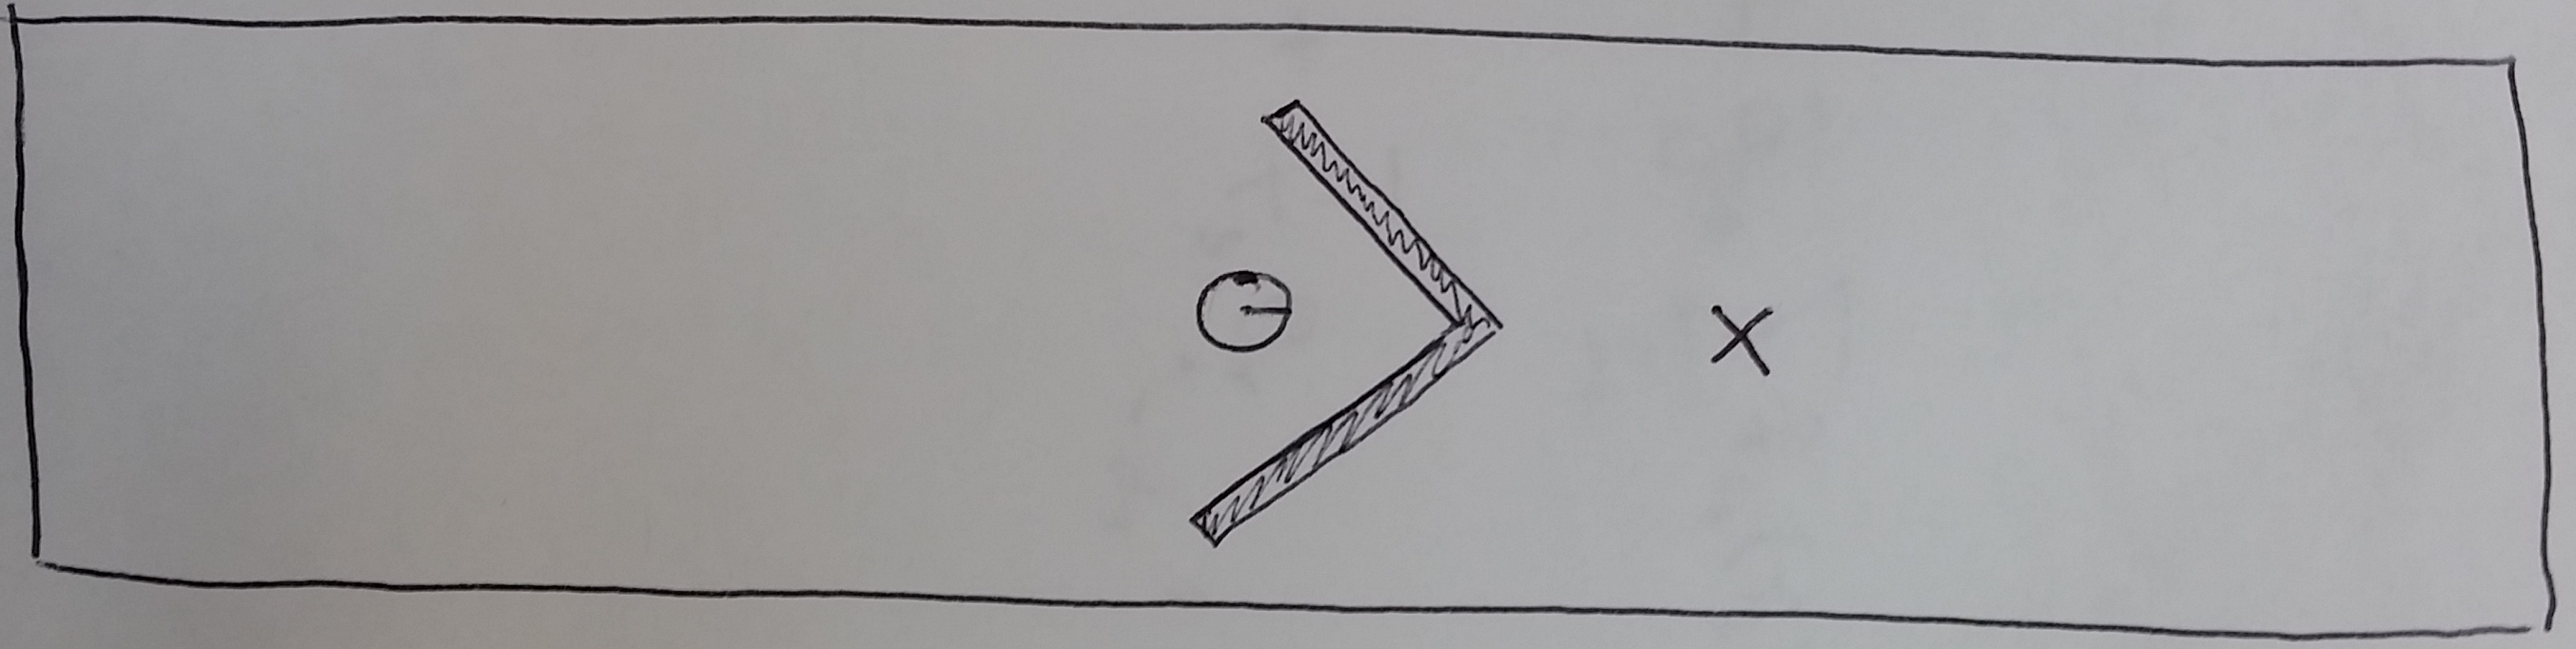
\includegraphics[width=\textwidth]{navtrap1.png}
	\caption
	{A degenerate case where the attractive force of the goal combines with the repulsive force of the wall producing a local optima
	where the robot gets trapped.}
	\label{fig:trap1}
\end{figure}

In such scenarios, an effective strategy to escape such traps is to randomly assign an alternate goal position $x_{rand}$
that will allow the robot to escape the local minima and proceed to the goal. The distance to $x_{rand}$ from the robot
is typically selected to be smaller than the distance to the nearest occlusion $\min(R)$. After some fixed time, the
goal position is set back to $x_g$. If the trap condition is detected multiple times then the next escape procedure is
repeated that many times before being restored to $x_g$. One possible method to detect a trap condition is to integrate
a sliding window of vehicle linear velocities $v_r$ and if those values integrate to a position close to zero then is is likely
that the robot has encountered a trap condition. It is shown in \cite{Krishnamurthy07} that with all of these mechanisms the position of the robot 
$x_r$ will converge to $x_g$ in finite time with probability 1.
	
%%%%%%%%%%%%%%%%%%%%%%%%%%%%%%%%%%%%%%%%%%%%%%%%%%%%%%%%%%%%%%%%%%%%%%%%%%%%%%%%%%
%%% Crawl Gait
%%% 
%%%
%%%%%%%%%%%%%%%%%%%%%%%%%%%%%%%%%%%%%%%%%%%%%%%%%%%%%%%%%%%%%%%%%%%%%%%%%%%%%%%%%%
\chapter{Humanoid Crawl Gait} \label{ch:crawl_gait}

Using the Nao platform, crawling gaits applicable to humanoid robots was explored. 
Not only is crawling a more stable gaiting strategy than walking, but it gives the robot access to areas
of the environment that are inaccessible via walking alone. A low-profile laterally symmetric crawl gait is described, 
modeling the robot as a closed-chain manipulator with pseudo-static dynamics. This gait was parameterized on 
three joint variables and optimized using a cubic splines approach via a genetic algorithm.

As was described in Chapter \ref{ch:navigation}, the gaiting modality directly affects the navigation strategy.
By selecting the appropriate gaiting strategy, the robot can modify its movement to achieve a commanded goal.
This modified movement also modifies which environmental objects present as obstacles.
Expanding the library of gaits legged robots have access to allows robots to be increasingly more capable
and applicable to a wider range of scenarios.
Griswald Brooks
\section{Humanoid Crawling}

Unlike walking and running which enjoy precise definitions, crawling seems to only have a subjective notion.
\cite{Dudek2000} asserts that crawling is a statically stable walk. This definition is problematic
as bipedal gaits have been demonstrated in \cite{figureoutacitation} that are statically stable but would not
be classified as crawling. In addition to this, soldiers performing the high army crawl \cite{armyfieldmanual2008} can be seen to
perform this motion very quickly which introduces a dynamic component to the crawl.
The standard or baby crawl is described as using one's hands and knees to produce forward motion.
In contrast to this, crawls such as the leopard, tiger, bear, and crab use hands and feet to produce
forward motion and the low army crawl uses the hands to drag and one leg to push the body across the ground.
Such diversity in crawling motion makes it difficult to differentiate a crawl from a statically stable
quadrupedal gait that uses something other than the end effectors to interact with the environment.
Despite this, the presented gait produces a motion that many would associate with humanoid crawling.

\subsection{Nao Crawling Limitations}

A primary limitation to the gaits that can be produced by the Nao is the limited number of degrees of freedom (DoF) of the platform
in contrast to the large number of DoF present in humans. While the Nao has 25 DoF, the human body has 244 \cite{zatsiorskybiomechanics}.
The human arm and leg each have 7 DoF while the Nao's arms and legs each have 5. 
Nao's hips have one more degree of freedom, called Hip Yaw-Pitch, which turn the legs together at an angle. 
Figure \ref{fig:nao_hips_legs1} illustrates this degree of freedom more clearly. 
The rest of the DoF of the Nao are in the hands and neck. 
Notably, Nao has no back joint. This prevents the gait designer from prescribing a twisting motion for use in the crawl gait.
These limits in motion preclude the execution of any gaits that require lateral twisting or sagittal arching.
Examples of this are shown in Figure \ref{fig:crawl_back1} .

\begin{figure}
	\vspace*{-0.07in}
	\centerline{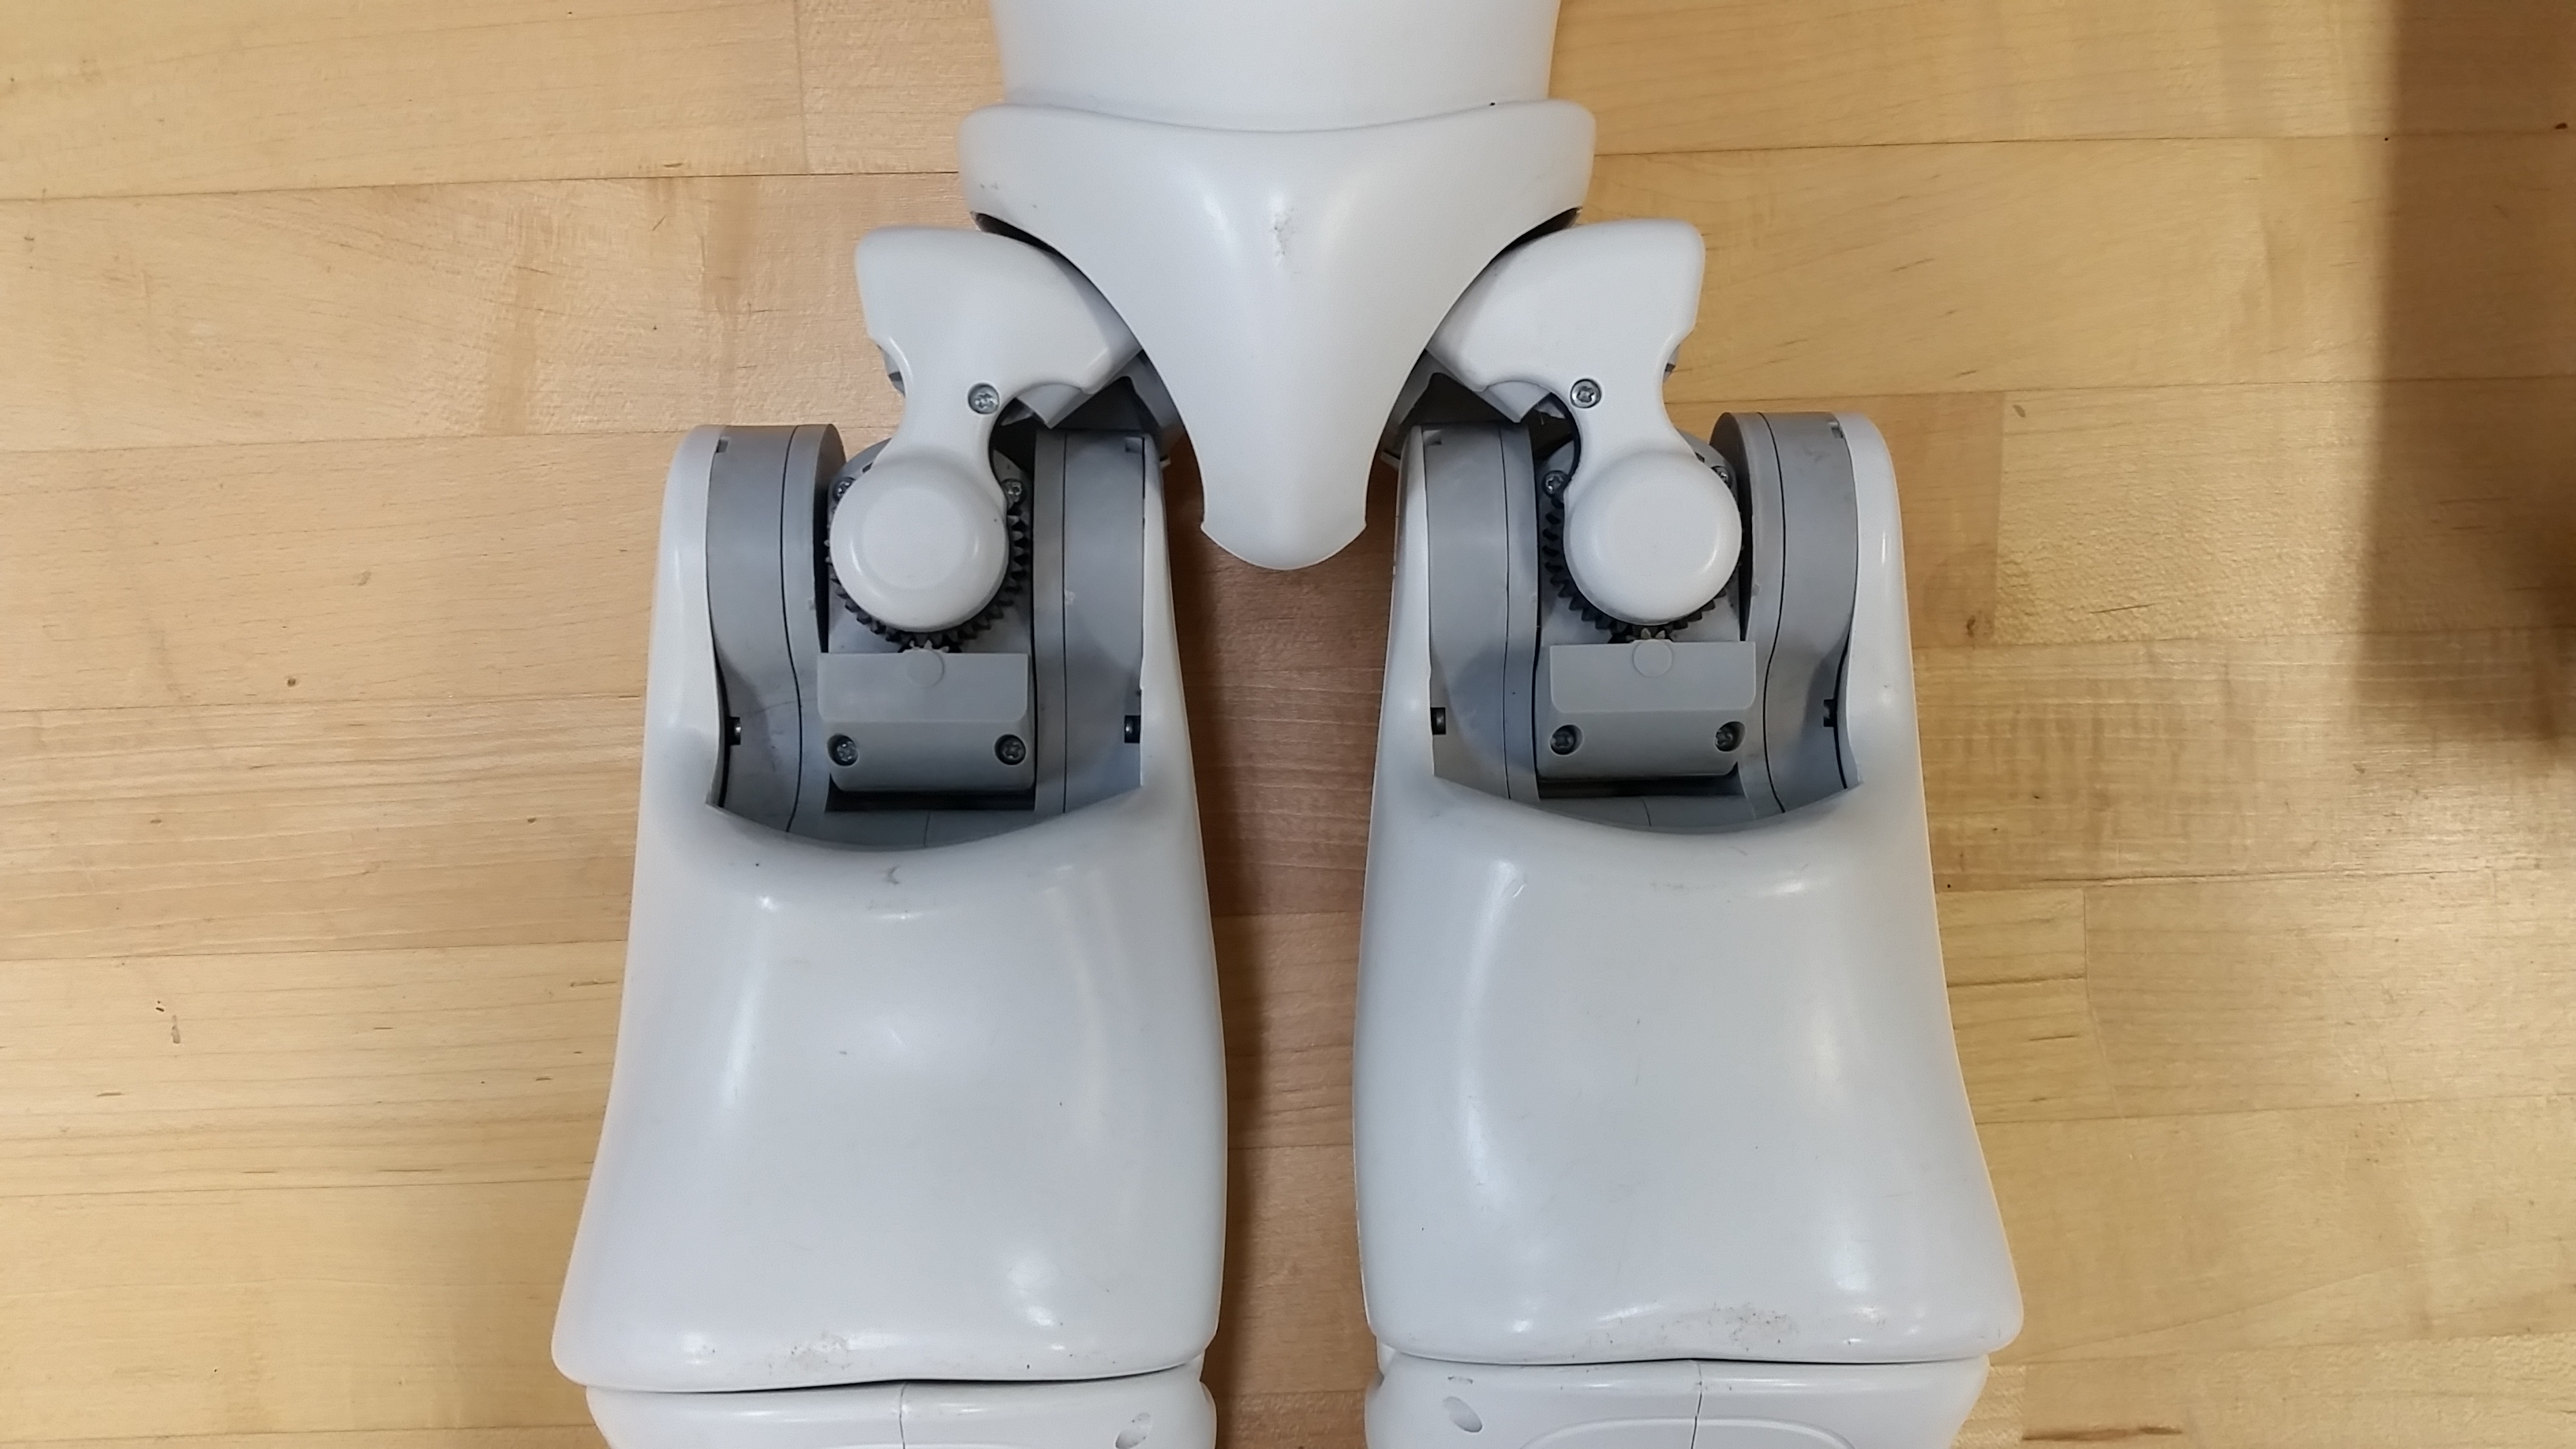
\includegraphics[width=0.395\textwidth]{nao_legs_together1.png}
				\includegraphics[width=0.5\textwidth]{nao_legs_spread1.png}
				}
	\caption{The pane on the left shows the leg configuration of the Nao when the Hip Yaw-Pitch DoF is fully turned in.
				The right pane show the leg configuration when the Hip Yaw-Pitch is fully turned out. 
				The legs are mechanically linked, making the amount of Hip Yaw-Pitch equal for each leg.}
	\label{fig:nao_hips_legs1}
	\vspace*{-0.2in}
\end{figure}

\begin{figure}
	\centering
	\includegraphics[width=\textwidth]{crawl_back_rough1.png}
	\caption
	{Illustration of crawl motions that involve actuated back joints. The left pane shows lateral twisting during a crawl.
		The right panes shows sagittal arching while on hands and knees.}
	\label{fig:crawl_back1}
\end{figure}

\section{Projected Profile Humanoid Crawl Gait}

The crawling gait presented in this thesis is based on viewing the humanoid form as a set of manipulators on the
sagittal plane. Figure \ref{fig:nao_sideview1} illustrates this concept.
When the robot is laying in the prone position, it necessarily makes contact with the ground. If we then view the robot
from the side (looking at the sagittal plane) we can model it as a planar kinematic chain. If the chest and knees
are making contact with the ground, then the arms from the shoulder joint to the hand, and the legs from the knees to the
toes are free to move without affecting the rest of the body. This produces two open chain manipulators. In the case of the Nao, each has two degrees
of freedom in the sagittal pane, allowing the hands and feet to move independently.
\begin{figure}
	\centering
	\includegraphics[width=\textwidth]{nao_pp_sagittal_view1.png}
	\caption
	{Illustration of Projected Profile concept. Both panes show the saggital view of the Nao with a schematic representation of the kinematics. 
	In the top view, the robot appears as two open chain manipulators. In the bottom view, the robot appears as one closed chain manipulator.}
	\label{fig:nao_sideview1}
\end{figure}

If the elbows and toes are placed on the ground, then the body from the toes to the elbow can be viewed as a closed chain manipulator.
This allows the joints to work together to move the center of mass. Kinematically, these two phases share two common configurations.
The first configuration is when the elbow is at full extension and the toes touching the knees. We will call this the ``extension" configuration.
This can be viewed as the robot reaching forward. The second is when the elbow is at full flexion and the ankles at extension.
We will call this ``compression".
This can be viewed as the robot having pulled itself forward. These motions can then be combined
to produce a full gait.

Using the Nao robot as an example, Figure \ref{fig:nao_phases1} shows the full gaiting sequence.
The robot initializes itself in the open chain configuration. From this, it can position
its end effectors (the toes and elbows) into the first common configuration ``extension". Next, the robot is in the closed chain 
configuration in which it can transport its center of mass forward until it reaches the ``compression" configuration. Finally the robot
is again in the open chain configuration and the cycle can start again.

\begin{figure}%[!th]
	\centerline{\includegraphics[width=0.5\textwidth]{White_Background/1_onBellyBegin.png}
				\includegraphics[width=0.5\textwidth]{White_Background/2_extension.png}
				}

	\vspace*{0.05in}

	\centerline{\includegraphics[width=0.5\textwidth]{White_Background/3_apex.png}
				\includegraphics[width=0.5\textwidth]{White_Background/5_onBellyEnd.png}
				}
	\caption{The above sequence shows the motion segments and robot postures in the crawl gait. 
				The upper left pane shows the initial open chain configuration. The upper right
				pane moves the robot to the ``extension" configuration. The lower left
				shows the ``compression" configuration. Finally, the lower right shows the 
				robot, having translated forward, once again in the open chain configuration.
				A 6-inch marker is shown in the background as a length scale reference.}
	\label{fig:nao_phases1}
\end{figure}

The gait is laterally symmetric. 
If we actuate the joints at an appropriate rate, dynamic effects from the robot's motion do not become a significant factor.
As detailed in Chapter \ref{ch:results}, this gait can be performed on the Nao at a speed of 1 ft every 6 to 8 seconds. 
The wide surface area of the forearm provides a high coefficient of friction against slipping and the small surface area of
the toes can act as a point of high pressure which can dig into soft surfaces such as carpets.
The gait is statically stable in the sense that the robot's motion can be paused at any point and the robot will maintain that pose.
The gait does not depend on the robot
sliding along the surface nor does it highly depend on surface friction to pull the robot forward.
The gait has a very low profile. The highest point on the robot during the gait (which is the top of the head)
is about 8 inches off of the ground. In contrast, during walking, the Nao robot stands 23 inches tall.

\subsection{Open Chain Kinematics}
The Projected Profile crawl gait has two kinematic configurations: open chain and closed chain. In the open chain
configuration, the robot acts as two independent planar manipulators. 
Each manipulator has two degrees of freedom as can be seen in Figure \ref{fig:open_chain1} .

\begin{figure}
	\centering
	\includegraphics[width=\textwidth]{stick_open_chain_rough1.png}
	\caption
	{Simplified kinematic model of the sagittal projection of the open chain configuration.
	The manipulator on the left represents the tibia-foot chain. The manipulator on the right
	represents the humerus-forearm chain. The origin of the knee and shoulder are represented as 
	having a z-axis offset because the knee and chest of the robot have heights that raise their 
	origins.}
	\label{fig:open_chain1}
\end{figure}

With the Nao facing downwards, the feet towards the origin and the head in the positive x direction, 
the forward kinematics for each manipulator are described by:
\begin{align}
	x &= x_0 + l_1 cos(\theta_1) + l_2 cos(\theta_1 + \theta_2) \\
	z &= z_0 + l_1 sin(\theta_1) + l_2 sin(\theta_1 + \theta_2)
\end{align}
where $x_0$ and $z_0$ are the superior and posterior offsets with respect to the global frame, respectively. $l_1$ is the length of the
humerus/tibia, $l_2$ is the length of the forearm/foot, $\theta_1$ is the angle subtended by the 
shoulder/knee and the x-axis, and $\theta_2$ is the angle subtended by the ankle/elbow and the x-axis of the humerus/tibia.

The solutions to the inverse kinematics problem can be seen as:

\begin{align}
	\theta_2 &= \cos^{-1} \left (\frac{(x - x_0)^2 + (z - z_0)^2 - l_1^2 - l_2^2}{2 l_1 l_2} \right ) \label{eq:open_fk_eq1}\\
	\theta_1 &= 2 \tan^{-1} \left (\frac{-B \pm \sqrt{B^2 - 4AC}}{2A} \right ) \label{eq:open_fk_eq2}\\
	A &= (x - x_0) + (z - z_0) + l_1 + l_2 (\cos(\theta_2) + \sin(\theta_2)) \\
	B &= -2(l_1 + l_2(\cos(\theta_2) - \sin(\theta_2)) \\
	C &= (x - x_0) + (z - z_0) - l_1 - l_2 (\cos(\theta_2) + \sin(\theta_2))
\end{align}

This solution derives from the standard inverse kinematics procedure of inverting the forward kinematics.
$\theta_1$ must be chosen such that no part of the robot tries to intersect with the floor. 
In practice, the two argument arc-tangent function $atan2$ is used instead of $\tan^{-1}$ .

%%% Projected profile %%%
\subsection{Closed Chain Kinematics}

The closed chain configuration models the toes and elbows of the robot as being fixed to the ground.
As with all closed chain kinematics, describing the forward kinematics requires solving an inverse
kinematics equation. Modeling the robot in the same orientation as the open chain, with the toe at the origin
and neglecting the thickness of the elbow,
the forward kinematics of the closed chain are:

\begin{align}
	d_e &= \sum_{i=1}^5 l_i \cos(\sum_{j=1}^i \theta_j) \label{eq:fk_eq1}\\
	0 &= \sum_{i=1}^5 l_i \sin(\sum_{j=1}^i \theta_j) \label{eq:fk_eq2} \\
	\alpha &=\sum_{i=1}^5 \theta_i \label{eq:fk_eq3}
\end{align}
where $d_e$ is the prescribed distance of the elbow from the foot and $\alpha$ is the desired angle
created by the x-axis of the humerus and the ground.
$\theta_1$ through $\theta_5$ are the angles of the following joints with respect to their previous links when projected onto the sagittal plane:
toe-to-ground, ankle, knee, hip, shoulder. In Figure \ref{fig:pp_stick1}, the red lines represent the links projected onto the sagittal plane.
These equations are the standard planar manipulation equations, treating the foot as the base link 
with the elbow as the end effector.
Equation \ref{eq:fk_eq1} constrains the end effector to be a set distance from the foot and 
equation \ref{eq:fk_eq2} constrains the end effector to be on the ground.
Using equation \ref{eq:fk_eq3}, equations \ref{eq:fk_eq1} and \ref{eq:fk_eq2} can be rewritten as:

\begin{align}
\sum_{i=1}^4 l_i \cos(\sum_{j=1}^i \theta_j) &= d_e - l_5 \cos(\alpha) \label{eq:sum_cos1} \\
\sum_{i=1}^4 l_i \sin(\sum_{j=1}^i \theta_j) &= - l_5 \sin(\alpha). \label{eq:sum_sin1}
\end{align}

\begin{figure}
	\centering
	\includegraphics[width=\textwidth]{stick3_with_notation1.png}
	\caption
	{Simplified kinematic model of the sagittal projection of the closed chain configuration.}
	\label{fig:pp_stick1}
\end{figure}

If $\theta_3$, $\theta_4$, and $\alpha$ are prescribed angles, then equations \ref{eq:sum_cos1} and \ref{eq:sum_sin1} are two equations 
in the two unknowns $\theta_1$ and $\theta_2$. 
$\theta_3$ and $\theta_4$ can be constant or time-varying as the resultant configuration is a function of these two ``free" variables.
Taking the square of each of the equations \ref{eq:sum_cos1} and \ref{eq:sum_sin1}, 
an equation in the single variable $\theta_2$ is obtained as:
\begin{align}
	2l_1 K_1 \cos(\theta_2) + 2l_1K_2 \sin(\theta_2) &= [d_e - l_5 \cos(\alpha)]^2 + [l_5 \sin(\alpha)]^2 - l_1^2 - K_1^2 - K_2^2 \label{eq:theta2_eq1} \\
	K_1 &= l_2 + l_3 \cos(\theta_3) + l_4 \cos(\theta_3 + \theta_4) \label{eq:theta2_eq2}\\
	K_2 &= -l_3 \sin(\theta_3) - l_4 \sin(\theta_3 + \theta_4) \label{eq:theta2_eq3}
\end{align}

The solution to equation \ref{eq:theta2_eq1} is of similar form to that seen in \ref{eq:open_fk_eq2}.
In general, there will be two solutions for $\theta_2$, but one of them will cause the robot to collide
with the ground and must be guarded against.
With $\theta_2$ solved, equations \ref{eq:sum_cos1} and \ref{eq:sum_sin1} can be used to solve for $\theta_1$:
\begin{align}
	\theta_1 = tan^{-1} \left( \frac{sin(\theta_1)}{cos(\theta_1)} \right ) \label{eq:theta1_eq1}\\
	cos(\theta_1) = \frac{K_3 (d_e - l_5 \cos(\alpha)) + l_5 K_4 \sin(\alpha)}{K_3^2 + K_4^2} \label{eq:theta1_eq2}\\
	sin(\theta_1) = \frac{K_4 (d_e - l_5 \cos(\alpha)) - l_5 K_3 \sin(\alpha)}{K_3^2 + K_4^2} \label{eq:theta1_eq3}\\
	K_3 = l_1 + K_1 cos(\theta_2) + K_2 sin(\theta_2) \label{eq:theta1_eq4}\\
	K_4 = K_2 cos(\theta_2) - K_1 sin(\theta_2) \label{eq:theta1_eq5}
\end{align}

Lastly, $\theta_5$ is solved using equation \ref{eq:fk_eq3}.

% Robot is like a parallelogram. Any robot that can make a parallelogram can use this principle.
With these angles solved, the entire robot is parameterized on three angles $\theta_3, \theta_4, \alpha$.
If $\theta_3$ and $\theta_4$ are fixed, then starting with the elbow at full extension, bringing the elbow
to flexion moves the robot forward. This corresponds to $\alpha$ starting with a small negative angle and 
ending with a large negative angle. 
For the Nao, $\alpha$ is initialized at approximately $-30^\circ$ and terminates at about $-90^\circ$ .
The primary intuition about this procedure is that the closed chain is like a parallelogram that is used to shift
the mass of the robot. Any robot (humanoid or not) that can be set into this configuration can use this 
framework in order to gait the robot.

\subsection{Nao Kinematics}
Once the projected profile time sequence of angles has been computed, it needs to be applied to the Nao.
Figure \ref{fig:nao_pp_view1} illustrates the sagittal view of the robot in the closed chain configuration.
When Nao is set to this configuration, the ankle pitch, knee pitch, hip pitch, and shoulder pitch joints 
of the robot directly correspond to $\theta_2$ through $\theta_5$. $\theta_1$ corresponds to the angle
subtended by the robot's foot and the ground. Unlike the first five joint angles, angle $\alpha$ does not have a
direct correspondence and the arm joint angles for shoulder roll $\theta_{sr}$, elbow yaw $\theta_{ey}$, 
and elbow roll $\theta_{er}$ must be derived as a relationship between the angle $\alpha$ and additional
arm positioning constraints.

\begin{figure}
	\includegraphics[width=\textwidth]{horz_profile_with_notation2.png}
  	\caption{Sagittal view the Nao in the closed chain crawling configuration. 
  				The locations of the joints used in the projected profile calculation are shown as blue dots. 
  				$n_p$ represents the sagittal plane of the robot.
  			}
  	\label{fig:nao_pp_view1}
\end{figure}

\begin{figure}
	\includegraphics[width=\textwidth]{hardware_rarmjoint_3.3.png}
  	\caption{Sagittal view the Nao in the closed chain crawling configuration. 
  				The locations of the joints used in the projected profile calculation are shown as blue dots. 
  				$n_p$ represents the sagittal plane of the robot.
  			}
  	\label{fig:nao_pp_view1}
\end{figure}

% [More to come on this part. Continue reading.]
% This is the part where we talk about the arm kinematics.
% Unlike the feet, etc, the arms are not inline with the rest of the body.
% We want to be able to position the arms a certain width apart to give a wider base and allow the elbows to
% rotate the projection of the forearm more before the actual forearm hits the humerus.

% The shoulder roll is computable as a function of the desired width, shoulder width, and the length of the humerus.
The shoulder roll $\theta_{sr}$ is computable as a function of 

The elbow roll is a function of the humerus vector and the desired forearm direction vector.
The elbow yaw is a function of the humerus vector, the desired forearm direction vector, and the axis of rotation
the the elbow roll revolves around.

With these three angles, the arm can be positioned.

To explain how to compute these, we have to define a whole bunch of vectors and scalars.
First the scalars.
Desired forearm-to-forearm spacing is denoted $d_f$.
The shoulder-to-shoulder spacing is denoted $d_s$
Then, as can be seen in one of the diagrams, we can define a quantity
$d = \frac{d_f - d_s}{2}$ as the y-component of the elbow, where the origin is placed at the shoulder joint,
the z-axis pointing up, x-axis facing forward.
$l_h$ is the length of the humerus.
$\tilde l_h = \sqrt{l_h^2 - d^2}$ is the length of the humerus, projected onto the z-x plane.

Now the vectors.
The first vector is the desired forearm orientation $u_f = [1, 0, 0]^T$. We want the forearm to lie on the ground
and pointing forward. On the ground to maximize surface contact so the robot is well supported and forward so the
ground contact is parallel to the direction of travel.
The next vector is the unit vector representing the direction that the humerus is pointing.
This vector represents the rotation axis for the elbow yaw joint on the Nao.
$v_{ey} = [\tilde l_h \cos(\alpha), d, \tilde l_h \sin(\alpha)]^T / l_h$.
As can be seen by Figure \ref{fig:nao_arm_vectors1} $[\tilde l_h \cos(\alpha), d, \tilde l_h \sin(\alpha)]^T$ represents
the humerus with the shoulder at the origin, which is then normalized by the length of the humerus $l_h$.
The next vector is the unit vector representing the rotation axis for the elbow roll joint on the Nao.
When the elbow yaw is zero, the rotation axis for the elbow roll is $v_{er} = [-\sin(\alpha), 0, \cos(\alpha)]^T$.
This vector $v_{er}$ is perpendicular to $v_{ey}$.

The goal here is to put the forearm to be $u_f$. When elbow yaw and elbow roll are zero, the orientation of the
forearm is coincident with the vector $v_{ey}$. We will denote the forearm vector as $v_f$ which is initialized to
$v_f = v_{ey}$.
In order to move $v_f$ to $u_f$ we have to rotate $v_f$ around $v_{ey}$ by an amount $\theta_{ey}$ and then about
$v_{er}$ by an amount $\theta_{er}$.

\begin{equation}
	u_f = R_{v_{er}, \theta_{er}} R_{v_{ey}, \theta_{ey}} v_f
\end{equation}

To find $\theta_{ey}$, we must first compute $v_f \times u_f$ to find the desired vector $u_{er}$ that
$v_{er}$ must be rotated to. Then, $\theta_{ey} = \arccos(v_{er} \cdot u_{er})$.
Then, $\theta_{er} = \arccos(v_{ey} \cdot u_f)$.

These four angles complete the arm kinematics and compute the joints angles given the projected profile angle $\alpha$
and the desired forearm-to-forearm spacing.

%%% Pseudo-static modelling %%%
\section{Optimization}

In the previous section, the Projected Profile crawl gait was parameterized on angle triplet 
$[ \theta_3, \theta_4, \alpha ]$ .
To achieve a crawling gait, $\theta_3$ and $\theta_4$ can be set to be constant and $\alpha$ linearly incremented
from an initial angle to a final angle as a function of time. While this configuration successfully gaits the robot,
it is heuristic. To improve the approach, the selection of a triplet of cubic splines 
$[\theta_3(t), \theta_4(t), \alpha(t)]$ is considered as an optimization problem. 
While many different quantities such as gait speed or the levelness of the back 
(for transportation of payloads) could be considered as optimization metrics, in this thesis the energy usage was 
minimized via joint torque measurements.
The aim was to increase the amount of time the crawling gait could be performed and reduce the stress on the robot's joints.

\subsection{Pseudo-static Model}

In order to optimize the gait with respect to the joint torques of the robot, a dynamic model of the robot is required.
As the Projected Profile crawl gait is conceived as a statically stable gait and performed at slow speeds,
the dynamics due to the movement of the robot are not considered to be forces that the 
motor controllers must counteract. 
During any part of the gait the robot will not slide if the gaiting direction is orthogonal to gravity and
if the robot were to relax its joints it would collapse.
Considering this, the resultant joint torques can be seen to be a function of gravity. 
This pseudo-static model of the robot can then be used to produce a cost metric for the optimization procedure.
While conceptually simple, analyzing the projected profile closed chain manipulator to produce the 
system dynamics is challenging.
In lieu of this, the robot was simulated for different values of the angle triplet in the closed chain 
configuration to generate a table of torques. This table of torques is then interpolated to produce
a model of joint torques as a function of the parameterized angles:
\begin{equation}
	[\tau_2, \tau_2, \tau_4, \tau_5] = jointTorques(\theta_3, \theta_4, \alpha)
\end{equation}
where $\tau_2, \tau_3, \tau_4, \tau_5$ are the torques of one of the ankles, knees, hips, and shoulders, respectively.
In this case, only one of each of the joints is considered because the gait is laterally symmetric. This means
the torque of the left joint should be the same of the right joint.
$\tau_1$ is not a product of the function as $\theta_1$ is not an actuated joint.

The V-REP simulator by Coppelia Robotics was used to gather joint torque data. It uses the Open Dynamics Engine (ODE)
as its dynamics solver and is distributed with a model of the Nao Humanoid Platform. The model of the Nao
kinematically corresponds with the Nao V4 and has the same mass values for the links. 
The Nao V4 is the robot used in this thesis.
It has an easy to use API that can interface with C++, Python, or MATLAB.

\begin{figure}
	\includegraphics[width=\textwidth]{nao_vrep1.png}
  	\caption{ A sample screen capture of the V-REP simulation of the Nao robot in the closed
  				chain configuration. The robot is set to different poses and then the joint torques
  				are read after a short settle time.
  			}
  	\label{fig:nao_vrep1}
\end{figure}

Figure \ref{fig:nao_vrep1} shows a screen capture of the Nao model in the V-REP simulator. 
The Nao was configured to be in the closed chain and set to different joints angles. 
The initial and final values of $\alpha$ were constrained due to the gaiting requirement of the elbow to start at 
extension and end at flexion. The ranges of $\theta_3$ and $\theta_4$ were defined according to what seemed
like plausible knee and hip angles for the gait. Using these limits a discrete set of triplets were defined
at a $2.5^\circ$ resolution for each triplet parameter. These triplets were sent through the kinematics equations to produce the joint
commands for the simulated Nao robot. 
Table \ref{tab:angle_set_params1} lists the parameters that describe the triplets tested. In total, 9,975
different joint configurations were simulated.
To allow for the effect of
any dynamics generated by the change in configuration to settle, the torque values of each of the joints was recorded
after a period of one second.

\begin{table}
	\centering
	\begin{tabularx}{0.65 \textwidth}{|X||X|X|}
		\hline
		\textbf{Configuration Parameter} 	&	\textbf{Minimum Angle (degrees)} 		&	\textbf{Maximum Angle (degrees)} 	\\	\hline\hline
		$\theta_3$ 	  & 	-5   &	 45 	\\	\hline
		$\theta_4$		&	  15	 &	-30	  \\ 	\hline
		$\alpha$			&  -30	 &	-90		\\ 	\hline
	\end{tabularx} 
	
	\caption{Table of initial and final joint angles for each angle in the configuration triplet used to generate the set of
				angles used to configure the simulated Nao robot.
				The resultant set had 9,975 configurations with an angular resolution of $2.5^\circ$.}
	\label{tab:angle_set_params1}
\end{table}

\subsection{Cost Functions} \label{subsec:cost_functions}

To find the optimal parameters for the angle triplet splines $[\theta_3(t), \theta_4(t), \alpha(t)]$, 
a cost $c_s$ has to be attributable to a given spline triplet as a function of the spline parameters.
The cost function contains terms regarding the joint torques given by the pseudo-static model, as
the primary goal of the optimization procedure is to reduce the overall usage of torque
(and therefore energy) of the gait. Additionally, a number of indicator functions
were introduced to the cost function in order to ensure kinematic constraints were not violated
and to deter problems with the algorithm's implementation, which will be discussed.

The cost function based on joint torques was computed as:
\begin{equation}
	c_{\tau}(t) = \sum_{i=1}^4 w_i \tau_i^2(t) \label{eq:cost_joint}
\end{equation}

In this notation, $\tau_1, \tau_2, \tau_3, \tau_4$ are the torques of the ankle, knee, hip, and shoulder, respectively.
These torques are taken from the pseudo-static model and, as stated, are a function of 
$\alpha(t), \theta_3(t),$ and $\theta_4(t)$.
The weight vector is constant and equal to $w = [1, 1, 1, 5]^T$.
$w_4$ has a higher value in order to reduce the use of Nao's shoulder, as its actuator can produce about 3 to 4 times
less torque than each of the leg actuators.

The first set of indicator functions introduced deter violation of kinematic constrains, such as joint limits
in $\theta_3$ and $\theta_4$ \ref{eq:fn_ind_theta}, starting and stopping conditions for $\alpha$ \ref{eq:fn_ind_alpha},
and to prevent the Nao from being in a kinematic configuration where the hips are making contact with the crawling
surface \ref{eq:fn_ind_z}.

\begin{align}
	c_{\theta_i}(t) &=
  	\begin{cases} 
  		\hfill 1 \hfill & \text{ if $\theta_i (t) > \theta_{i_{max}}$ or $\theta_i (t) < \theta_{i_{min}}$ } \\
    	\hfill 0 \hfill & \text{ otherwise }
  	\end{cases} \label{eq:fn_ind_theta} \\
  c_{\alpha}(t) &=
  	\begin{cases} 
    	\hfill 1 \hfill & \text{ if $\alpha(t) > \alpha_{max}$ or $\alpha(t) < \alpha_{min}$ } \\
      \hfill 0 \hfill & \text{ otherwise }
  	\end{cases} \label{eq:fn_ind_alpha} \\
	c_{z_{hip}}(t) &=
  	\begin{cases} 
    	\hfill 1 \hfill & \text{ if $z_{hip}(t) < z_{hip_{thresh}}$ } \\
      \hfill 0 \hfill & \text{ otherwise }
  	\end{cases} \label{eq:fn_ind_z}
\end{align}

The function $z_{hip}(t)$ returns the height of the hips at time $t$ using the the forward kinematics of the
closed chain model of the gait. $z_{hip_{thresh}} \ne 0$, and is chosen to be the height of the hip joint when
the robot is touching the crawling surface.

The next indicator function exists to deter a problem observed with the gaits being produced. 
Experimentally, it was seen that the optimizer would produce splines in which the parameter
$\alpha$ would, for a large part of the gait, either stay nearly stationary or increase for some time, before
decreasing by a large amount.
To review, $\alpha$ is initialized at approximately $-30^\circ$ and terminates at about $-90^\circ$.
This appeared as the robot lunging forward at the end of the gait.
This can most readily intepreted as the robot incurring a large cost for a small time, which is perhaps
a local optima. An indicator function \ref{eq:fn_ind_dalpha} was added to penalize splines in which 
$\alpha (t)$ was not monotonically decreasing, which allowed the optimizer to find a more efficient gait.

\begin{equation} 
	c_{\dot \alpha}(t) =
  	\begin{cases} 
    	\hfill 1 \hfill & \text{ if $\dot \alpha(t) \ge 0$ } \\
      \hfill 0 \hfill & \text{ otherwise }
  	\end{cases} \label{eq:fn_ind_dalpha}
\end{equation}

The indicator functions are then summed and multiplied by a large constant $C_v$ so that the cost to
violate any of these constraints is prohibitively large.

\begin{equation}
	c_I(t) = C_v \Big( c_{\dot \alpha}(t) + c_{\alpha}(t) + c_{z_{hip}}(t) + \sum_3^4 c_{\theta_i}(t) \Big) \label{eq:cost_ind}
\end{equation}

The cost of the spline triplet is then given by integrating the sum of cost functions \ref{eq:cost_joint} and
\ref{eq:cost_ind}, and can be seen in equation \ref{eq:cost_spline}.

\begin{equation}
c_s = \int_0^T c_{\tau}(t) + c_I(t) \, dt \label{eq:cost_spline}
\end{equation}

where $T$ is equal to one second, as it was seen that this was a reasonable time frame for this phase of the gait
to be performed. 

\subsection{Optimization Procedure}

The optimization procedure used to optimize the spline triplet $[\theta_3(t), \theta_4(t), \alpha(t)]$
was a basic genetic algorithm implemented using the genetic algorithm functions available in the MATLAB 
Global Optimization Toolbox. 

Briefly, genetic algorithm optimization works by first creating a ``population'' of
possible solutions, in this case the parameters for the spline triplet. Then the ``fitness'' of each solution
is determined, here by evaluating the cost function for the solution. Finally, the solutions that are more fit
are ``selected'' to for the ``parent'' set. These parents are then ``bred'' to form a new set of ``child'' solutions
which will then be evaluated again. After some number of ``generations'', the most fit solution is selected
as the optimal solution.

Genetic algorithms are well suited for problems like this as more classical optimization techniques
would require the cost function to be analytical, which the joint torque table is not.
As a result, because there is so much freedom in the cost function, different functions can be tried
and evaluated to find a suitable result.
Lastly, because the gait design problem presented in this thesis, was not required to run in real time on the
Nao, using such a computationally heavy optimization technique did not impact gait performance.
One pitfall to this technique is there is no guarantee that the global optima will be found for
a given cost function and therefore local optima are still possible to be returned.

Using the cost function presented in Section \ref{subsec:cost_functions}, the genetic algorithm was used
to find the 12 triplet parameters (4 parameters for each cubic spline). The algorithm ran for 67 generations
and produced a triplet spline whose cost was approximately six times smaller than the nominal strategy
of holding $\theta_3$ and $\theta_4$ constant while linearly increasing $\alpha$.
	% \include{./chapters/simulations}
	%%%%%%%%%%%%%%%%%%%%%%%%%%%%%%%%%%%%%%%%%%%%%%%%%%%%%%%%%%%%%%%%%%%%%%%%%%%%%%%%%%
%%% Navigation
%%% 
%%%
%%%%%%%%%%%%%%%%%%%%%%%%%%%%%%%%%%%%%%%%%%%%%%%%%%%%%%%%%%%%%%%%%%%%%%%%%%%%%%%%%%
\chapter{Navigation Results} \label{ch:results_navigation}

% The structure of this chapter needs revision.

% What do we have to talk about here?
% Well, I suppose the point of this chapter is to present how well the algorithm worked.
% What is there to present?
% I suppose it should be shown that the algorithm does indeed nav the robot,
% as that is not necessarily assumed in the chapter explaining the navigation.
% Some things you might want to know:
% Qualitatively, how well did it nav the robot?

% Ok, so what can I show?
% I can show pictures of the Nao naving around different environments getting to goals
% I can show what the robot thought his pose was based on the goal.
% I can list the optimal parameters for naving.
% I wish I could have shown laser data, because maybe I could have shown a potential field map.
% Can I show the different parts of what the nav was using? No, because the straight line planner
% and escape strategy was not implemented.

\section{Intro/Experimental Setup}
As mentioned in Chapter \ref{ch:platform}, in order to test the GOZILA algorithm,
the Nao was used, and had a Hokuyo LIDAR stuck to its chest.
We used Nao's built in walking to walk, which as we'll discuss, sucked (put us at a disadvantage),
because since we strapped a big mass to it's chest that it didn't know about,
the thing had a tendency to loose stability and fall over.
(In fact we couldn't keep going because the fucker kept falling over and breaking it's gears.)

The LIDAR allowed the Nao to detect obstacles. These LIDAR points fed the algorithm and repelled.

Also, since we needed to know where the goal was we used the built it blob
detection on Nao and made up a big red cube for it to detect.
The stock blob detection not only gives you bearing to a goal but it also assumes that the
red blob is a certain size (diameter: 0.06 m) and therefore can estimate range to the obstacle.
While you would think then that we should have used an object that size,
since we were asking it to track something so far away and cameras suck, we had to use a bigger (0.127 m or 5 inch
side length or twice as big)
object so it could be seen at distance.
This of course then meant that the range measurement was incorrect, but since we were
only using the range measurement for the goal attraction and to determine when to stop,
it wasn't that big of a deal and we could tune around it.
Now that I think about it, what we should have done was calibrate the distance with this
object so the tuning for GODZILA and the stopping distance would be ``real'' and not to
this messed up thing.
You would definitely definitely definitely have to do this if you were going to do mapping,
which was the next step.

The outer perimeter of the arena way yay big. The LIDAR range was 5 meters, so having the
perimeter, which was all straight flat walls, meant that the robot could always see them.
This let things be consistent when testing, thought not strictly necessary for the algorithm to
work as the robot doesn't need to localize in order to navigate.
You don't see these walls in the figures, for aesthetic reasons.

Hey! Also! The whole thing was recorded with a global camera (A GoPro).
Having a fixed camera like this is good because it makes tracking the robot
to measure it's performance trivial.
We used some image processing to track the Nao's orangeness, clustered to
find the Nao-like things that were being tracked in the image,
and then fit a 5th order polynomial curve to it to estimate the path of the
robot.

All in all, you can see that the robot makes it to the goal.
It has a hard time in some places, but this isn't because of the algorithm,
it's because of the balance issues with the LIDAR and the walking.
You can see this a lot in the narrow example on the left side of the aperture where the
robot oscillates a lot, but in general you can see a periodic amplitude (?) thoughout 
the entire gait which is not normal to the walking gait and being caused by the
instability introduced (though obviously there is some normal amount of periodicity
to any walking gait but it shouldn't be THAT bad).

Somewhere we should mention that this method only works if the shape of the field is
convex. The potential field method is subject to local minima (the U-shape mentioned in Chapter
\ref{ch:navigaiton} is a good example). It would be the job of the escape strategy to
try and break out of this.

The escape strategy is a bit tough because detecting ``stuckedness'' is tough in long
limit cycles without mapping.
In local minima that cause the robot to more or less stop, you can try and detect that
the distance to the goal hasn't reduced in awhile.
This was mentioned in Chapter \ref{subsec:escape_strategy}.

\subsection{Ok, so then where did we test this?}
We did three different environments with different environmental features.
So, as a control basically, one of the environments was just open. Yes there are walls
so there is a repulsive force but nothing should be obstructing the attraction to the
goal and if this doesn't work then something is really messed up. Figure \ref{fig:nav_open_setup1}
shows the setup.

\begin{figure}
  \includegraphics[width=\textwidth]{nav/open/no_path/frame1.png}
  \caption{Here's the open arena. Robot on left. Goal is the red boxy thing on the right.
           There's a bunch of walls that the robot can also see. Those same walls will
           always be there in all of the setups.}
  \label{fig:nav_open_setup1}
\end{figure}

Next we tried one that had a narrow opening between the robot and the goal.
The aperture is about 73 cm wide.
This aperture is about 2.6 times the width of the body of the robot (27.5 cm wide).
It was more or less the
limit of this approach because if we allow the robot to get closer to obstacles it tends
to cut too close to corners and other things and mess up.
To solve this, you'd need something that plans paths though these narrow but traversable
areas and have intermediate goals along this path for GODZILA to use.
These would then ``pull'' the robot through the narrow aperture.
This is how the straight line planner works when the goal is in sight.
That's not the case in the setup so the straight line planner cannot be invoked.
Also, that's again not really the focus of this algorithm and as mentioned in
Chapter \ref{ch:navigation}, the responsibility of some global planner.
Figure \ref{fig:nav_narrow_setup1} shows the setup.

\begin{figure}
  \includegraphics[width=\textwidth]{nav/narrow/no_path/frame1.png}
  \caption{Here's the arena with the narrow opening.
           The opening is about 2.6 times the width of the robot.
           This is pretty much the minimum aperture width this method can allow.}
  \label{fig:nav_narrow_setup1}
\end{figure}

Finally, we invoked a more complicated geometry where the robot had to go around
a large obstacle. In this case, the robot is always relatively close to obstacles and the
being pushed. Despite the constant repulsion, the goal is attractive enough to
pull the robot to the goal. Figure \ref{fig:nav_square_setup1} shows the setup.

\begin{figure}
  \includegraphics[width=\textwidth]{nav/square/no_path/frame1.png}
  \caption{This is the arena with the large obstacle.
           In this case, there's an obstacle closer to the robot than the goal most of the time.
           The hallway is about as narrow as you can make it.}
  \label{fig:nav_square_setup1}
\end{figure}

\subsection{How was the test setup constructed?}
Everything was boxy since that was the easiest shape to put together that had the
same 2D projection throughout. We could only test things at laser height and obstacles
like chairs which can have things jutting out above and below the laser are obviously going
to mess things up because the robot can't see them, so there really wasn't a point to testing
that.
Maybe we could have had more thin objects but then we're talking about the laser resolution
constraint. This would probably be a good one to try next time since it falls in the range of
detectability though it's sort of now in the obstacle avoidance part of things
which should be it's own algorithm in the stack of things to do all of navigation.

The robot was told to stop 0.3 meters radius from the goal.

\section{Parameter stuff}
WHAT ARE THE OPTIMAL PARAMETERS/PARAMETERS USED.
Table \ref{tab:nav_params1} shows the parameters used.
This table will have to be reduced and most likely added to the appendix in it's
full form. Also, probably going to have to explain all of these parameters.
Probably something like, ``we interface with/tune the algorithm through the following parameter''
and then explain each one in relation to the math or whatever.

\begin{table}
  \centering
  \begin{tabularx}{0.65 \textwidth}{|X||X|}
    \hline
    \textbf{Configuration Parameter}  & \textbf{Minimum Angle (degrees)}\\  \hline\hline
    goalStoppingRadius        &   0.3   \\  \hline
    vmin                      &   -0.4  \\  \hline
    vmax                      &   0.4   \\  \hline
    wmin                      &  -0.2   \\  \hline
    wmax                      &   0.2   \\  \hline
    clearanceThreshold        &   0.3   \\  \hline
    obstacleThreshold         &   3     \\  \hline
    goalAttraction            &   100   \\  \hline
    obstacleRepulsionTurning  &   20    \\  \hline
    obstacleAttraction        &   0     \\  \hline
    obstacleGoalBearingRatio  &   1     \\  \hline
    vehicleInertia            &   15    \\  \hline
    velocityGain              &   5     \\  \hline
    obstacleRepulsionForward  &   5     \\  \hline
    angularRateBraking        &   3     \\  \hline
  \end{tabularx} 
  
  \caption{These are the parameters we used. They worked pretty well.}
  \label{tab:nav_params1}
\end{table}

\textbf{goalStoppingRadius}        \\
The radius at which the robot considers itself at the goal.

\textbf{clearanceThreshold} \\
Method for setting the minimum acceptable distance between the vehicle and an obstacle.
Setting this distance does not guarantee that the robot will never violate this threshold.
Distance from the center of the robot to the center of an obstacle in meters. 
This distance is center to center because all objects are modeled as points. \\

\textbf{obstacleThreshold}         \\
Method for setting the obstacle range at which it is acceptable to treat obstacles
as attractive rather than repulsive.
Obstacle range threshold measured in meters. \\

\textbf{TUNING ANGULAR} \\
Method for tuning the planning parameters for angular velocity. \\

\textbf{goalAttraction}            \\
Tunes the strength of goal attraction.
Larger values increase attraction strength. \\

\textbf{obstacleRepulsionTurning}  \\
Tunes the strength of obstacle repulsion for 
obstacles closer than the obstacle range threshold.
Larger values increase repulsion strength. \\

\textbf{obstacleAttraction}        \\
Tunes the strength of obstacle attraction for 
obstacles farther than the obstacle range threshold.
Larger values increase attraction strength. \\

\textbf{obstacleGoalBearingRatio}  \\
Tunes the trade off between avoiding obstacles 
which are in the vehicle's current direction 
of travel versus avoiding objects which are 
in the direction of the goal.
This parameters ranges from 1 to 0. 
Values closer to 1 amplify the avoidance of 
obstacles in the direction of travel.
Values closer to 0 amplify the avoidance of 
obstacles in the direction of the goal. \\

\textbf{vehicleInertia}            \\
Tunes the strength of the vehicle's resistance 
to turning. Larger values mean more resistance.

\textbf{TUNE LINEAR}
 Method for tuning the planning parameters for linear velocity.
\textbf{velocityGain}              \\
Tunes the aggressiveness of the linear velocity. 
Larger number produces more aggressiveness. \\

\textbf{obstacleRepulsionForward}  \\
Tunes the strength of obstacle repulsion.
Larger values increase repulsion strength.\\

\textbf{angularRateBraking}        \\
Tunes the amount by which high turning rates reduce linear velocity.
Larger values reduce linear velocity. \\


\section{Picture of the Nao navigating}

Basically, these pictures are here just to show you that the robot
made it through the environment. It's not strictly necessary but you wouldn't
believe me otherwise and they're pretty to look at.
For convenience, I overlaid the best fit path from the image analysis just
so you could see ``where'' Nao was going and to give continuity to what you
are looking at.

\begin{figure}
  \centerline{
    \includegraphics[width=0.5\textwidth]{nav/open/path/open_path1.png}
    \includegraphics[width=0.5\textwidth]{nav/open/path/open_path2.png}
  }
  \vspace*{0.05in}
  \centerline{
    \includegraphics[width=0.5\textwidth]{nav/open/path/open_path3.png}
    \includegraphics[width=0.5\textwidth]{nav/open/path/open_path4.png}
  }
  \caption{This guy shows the Nao walking to the goal in the open area.
           The robot basically walks in a straight line, which is what you'd expect.}
  \label{fig:nav_open_frames1}
  \vspace*{-0.07in}
\end{figure}

\begin{figure}
  \centerline{
    \includegraphics[width=0.5\textwidth]{nav/narrow/path/narrow_path1.png}
    \includegraphics[width=0.5\textwidth]{nav/narrow/path/narrow_path2.png}
  }
  \vspace*{0.05in}
  \centerline{
    \includegraphics[width=0.5\textwidth]{nav/narrow/path/narrow_path3.png}
    \includegraphics[width=0.5\textwidth]{nav/narrow/path/narrow_path4.png}
  }
    \caption{This one shows the robot walking through the narrow aperture.
             You can see that the robot walks more or less straight the the opening and then to the goal.}
    \label{fig:nav_narrow_frames1}
        \vspace*{-0.07in}
\end{figure}

\begin{figure}
  \centerline{
    \includegraphics[width=0.5\textwidth]{nav/square/path/square_path1.png}
    \includegraphics[width=0.5\textwidth]{nav/square/path/square_path2.png}
  }
  \vspace*{0.05in}
  \centerline{
    \includegraphics[width=0.5\textwidth]{nav/square/path/square_path3.png}
    \includegraphics[width=0.5\textwidth]{nav/square/path/square_path4.png}
  }
    \caption{This figure shows the robot walking around a large obstacle.
             The robot walks down the corridor to the goal.}
    \label{fig:nav_square_frames1}
        \vspace*{-0.07in}
\end{figure}

\section{The plots from the global camera tracking}
These are what comes out of the image processing.
I guess I should tell you that I used OpenCV to do blob tracking, some dilations, near cluster
joining (like the head and shoulders show up as 3 orange blobs so they are joined to estimate the
center of the robot), then density based clustering to see which ones belong to which (the red cube is
orange enough to register as something to track so instead of trying to tune the fuck out of the colors
or use some other technique like template-matching or something I don't know about yet since I'm just 
starting to use OpenCV), I opted to do clustering and then I manually select which cluster of points are
the Nao's. Then I used a 5th order polynomial to fit the path.

Again, I'm not really sure why you need to see this other than to say here's an analysis of 
what the robot did that's a little more than just straight pictures.
You can really see the periodicity in the gait on these graphs.

You should notice here that while the robot was told to stop at 0.3 m, it actually
stops closer to 0.8 m from the goal.
This is because of the mismatch between how big the robot thinks the red object is
and the fact that it's about twice as big.

\begin{figure}
  \includegraphics[height=0.5\textheight]{nav/open/plots/nav_open.png}
  \caption{Here's a plot of the robot as seen by the video and the best fit path, in the open area.
           You can really see the wobble here caused by the LIDAR + gait mismatch.
           The starting point is the red square on the left and the goal is the yellow star on the right.
           The robot was told to stop at some radius to the goal.}
  \label{fig:nav_open_plot1}
\end{figure}

\begin{figure}
  \includegraphics[height=0.5\textheight]{nav/narrow/plots/nav_narrow.png}
  \caption{Here's the plot of the robot walking through the narrow aperture.
           The robot had a lot of trouble at the opening of the aperture which can be seen by the
           large smattering of points in the $(1.4, 0.75)$ region. Again, this is because of
           the mismatch.}
  \label{fig:nav_narrow_plot1}
\end{figure}

\begin{figure}
  \includegraphics[height=0.5\textheight]{nav/square/plots/nav_square.png}
  \caption{Here's the plot of the robot walking around the square obstacle. It does pretty well.}
  \label{fig:nav_square_plot1}
\end{figure}

\section{What Nao Saw of the Goal}

I REALLY have no idea what these are suppose to do for you, but here they are.
This is what the Nao ``saw'' of the goal while it was walking.
The ranges are asymptotically decreasing like you would think they would do if the robot
was getting closer. This doesn't technically have to happen if the robot can ``slide''
along a straight wall for awhile where it could get a little longer for a bit or in a situation
where the range stays constant for awhile like a radial wall?
One thing to note is though that the range could never really increase significantly.
Like if the robot had to go around something that made it walk away, that would never happen.
The robot would be stuck in this local minima like we talked about in one of the sections of Chapter
\ref{ch:navigation}.
We'd have to use some sort of escape strategy.

The angle doesn't really tell you much since it's the relative bearing which is important to the robot
but hard for use to interpret since we don't know the global orientation of the robot.
Actually, since the goal is not moving, then we probably could do better with the orientation data
to tell us the orientation of the robot. It's not worth it for this thesis but we could run it through
some filters and get something to work. We'd either have to EKF it with the initial pose or PF it.
Not really part of the thesis, but then it makes sense to have analyzed the data because then we could
use it as the ground truth for a localization algorithm (like Agraj did).
The best we can say is that in one of them (the open area one which makes sense since it had plenty of
time to get a lock on things and ride the pipe in) it's like always decreasing so he's homing in on things
and in the others it's oscillating back and forth so it's marginally stable or
looks like it's some other type of stability like lyapunov or some other thing, which you could
say means he's got a good track on things.

I mentioned before that the robot was commanded to stop at 0.3 meters but actually stops closer
to 0.8 meters because of the perception mismatch.
In the figures \ref{fig:nav_open_rb1}, \ref{fig:nav_narrow_rb1}, and \ref{fig:nav_square_rb1},
you can see that the robot thinks it's stopping at the appropriate distance
of 0.3 meters.

\begin{figure}
  \includegraphics[height=0.5\textheight]{nav/open/tracking/open_rb1.png}
  \caption{This is what the robot saw in the open area.
           The range decreased like you'd expect and the bearing is basically working its way
           to convergence for a lot of it because the robot had time to do so.}
  \label{fig:nav_open_rb1}
\end{figure}

\begin{figure}
  \includegraphics[height=0.5\textheight]{nav/narrow/tracking/narrow_rb1.png}
  \caption{Here's what the robot saw during the narrow aperture run.
           Again, the range decreases but the bearing doesn't.
           This is fine because the robot is moving and turning and stuff so the bearing
           won't really converge.}
  \label{fig:nav_narrow_rb1}
\end{figure}

\begin{figure}
  \includegraphics[height=0.5\textheight]{nav/square/tracking/square_rb1.png}
  \caption{This is what the robot saw during the large obstacle run.
           It basically has the same behavior as the other one.}
  \label{fig:nav_square_rb1}
\end{figure}
	% %%%%%%%%%%%%%%%%%%%%%%%%%%%%%%%%%%%%%%%%%%%%%%%%%%%%%%%%%%%%%%%%%%%%%%%%%%%%%%%%%%
%%% Crawl Gait
%%% 
%%%
%%%%%%%%%%%%%%%%%%%%%%%%%%%%%%%%%%%%%%%%%%%%%%%%%%%%%%%%%%%%%%%%%%%%%%%%%%%%%%%%%%
\chapter{Crawl Gait Results} \label{ch:results_crawl_gait}

% The structure of this chapter needs revision.

% What do we have to talk about here?
% Well, I suppose the point of this chapter is to present how well the algorithm worked.
% What is there to present?
% I suppose it should be shown that the crawl gait does indeed crawl the robot,
% as that is not necessarily assumed in the chapter explaining the gait.
% Some things you might want to know:
% How fast did the robot go?
% How high?
% What was the torque usage?

Crap I have to say about crawling.

PUT A PROJECTED PROFILE PICTURE HERE FOR THE INTRO.

THESE ARE ALL DONE WITH THE TRIVIAL TRIPLET PARAMETERS.

Explain the gait and it's parameters.

Explain the different experimental setups.

Explain that the point of this setup is to show that the crawl gait is very low profile.
\begin{figure}
  \vspace*{0.02in}
  \centerline{
    \includegraphics[width=0.25\textwidth]{crawl/under_table/14s.png}
    \includegraphics[width=0.25\textwidth]{crawl/under_table/18s.png}
    \includegraphics[width=0.25\textwidth]{crawl/under_table/19s.png}
    \includegraphics[width=0.25\textwidth]{crawl/under_table/20s.png}
  }
  \caption{Low-profile crawling gait for accessing vertically constrained spaces such as under a table.}
  \label{fig:nao_crawl1}
  \vspace*{-0.07in}
\end{figure}

Explain that this experiment is a demonstration of the gait being used to perform a task,
getting through a crawl space.

\begin{figure}
  \centerline{
    \includegraphics[width=0.2\textwidth]{crawl/walk_to/to/12s.png}
    \includegraphics[width=0.2\textwidth]{crawl/walk_to/to/18s.png}
    \includegraphics[width=0.2\textwidth]{crawl/walk_to/to/29s.png}
    \includegraphics[width=0.2\textwidth]{crawl/walk_to/to/30s_2.png}
    \includegraphics[width=0.2\textwidth]{crawl/walk_to/to/34s.png}
  }
  \vspace*{0.05in}
  \centerline{
    \includegraphics[width=0.2\textwidth]{crawl/walk_to/to/37s.png}
    \includegraphics[width=0.2\textwidth]{crawl/walk_to/to/40s.png}
    \includegraphics[width=0.2\textwidth]{crawl/walk_to/to/41s.png}
    \includegraphics[width=0.2\textwidth]{crawl/walk_to/to/43s.png}
    \includegraphics[width=0.2\textwidth]{crawl/walk_to/to/46s.png}
  }
  \vspace*{-0.05in}
  \caption{BLAH BLAH Approaching and crawling under an obstacle.
           A red dot is used as a marker for the direction in which the robot is commanded to move.
           When the robot approaches below a specified distance threshold from the obstacle,
           the crouch-down and crawl gait sequence is initiated.}
  \label{fig:nao_crawl3}
  \vspace*{-0.15in}
\end{figure}

\begin{figure}
  \centerline{
    \includegraphics[width=0.2\textwidth]{crawl/walk_to/from/8s.png}
    \includegraphics[width=0.2\textwidth]{crawl/walk_to/from/15s.png}
    \includegraphics[width=0.2\textwidth]{crawl/walk_to/from/16s.png}
    \includegraphics[width=0.2\textwidth]{crawl/walk_to/from/17s.png}
    \includegraphics[width=0.2\textwidth]{crawl/walk_to/from/18s.png}
  }
  \vspace*{0.05in}
  \centerline{
    \includegraphics[width=0.2\textwidth]{crawl/walk_to/from/24s.png}
    \includegraphics[width=0.2\textwidth]{crawl/walk_to/from/30s.png}
    \includegraphics[width=0.2\textwidth]{crawl/walk_to/from/32s.png}
    \includegraphics[width=0.2\textwidth]{crawl/walk_to/from/35s.png}
    \includegraphics[width=0.2\textwidth]{crawl/walk_to/from/37s.png}
  }
  \vspace*{-0.05in}
  \caption{BLAH BLAH Crawling under an obstacle and transitioning back to stand posture.}
  \label{fig:nao_crawl4}
  \vspace*{-0.01in}
  \vspace*{-0.05in}
\end{figure}

Here is a plot of the joint angles of the gait, showing its periodicity.

\begin{figure}
  \centerline{
    \includegraphics[width=0.5\textwidth]{crawl/joint_angles/LeftArmJointAngles.png}
    \includegraphics[width=0.5\textwidth]{crawl/joint_angles/LeftLegJointAngles.png}
  }
  \vspace*{-0.05in}
  \caption{Measured motor joint angles during multiple iterations of the periodic crawling gait.
           While the crawling gait is laterally symmetric, the asymmetry in measured angles is due to the
           definitions of the robot frame and joint frame in the NAO API, which essentially forms a mirror
           asymmetry between the left and right joints.}
  \label{fig:nao_joint_angles1}
  \vspace*{-0.1in}
\end{figure}

This is a full plot of the entire sequence, from walking, to crawling, to walking.

\begin{figure}
  \centerline{
    \includegraphics[width=0.5\textwidth]{crawl/joint_angles_long_sequence/LeftArmJointAngles_longSequence.png}
    \includegraphics[width=0.5\textwidth]{crawl/joint_angles_long_sequence/LeftLegJointAngles_longSequence.png}
  }
  \vspace*{-0.05in}
  \caption{Measured joint angles for a sequence of transitioning from standing to crouch to crawling,
           crawling under a table, and then returning to crouch.}
  \label{fig:nao_joint_angles_long_seq}
  \vspace*{-0.2in}
\end{figure}

This plot shows the current draws of the arm and leg joints.
There are some distinct patterns, but is hard to relate torques directly.

\begin{figure}
  \centerline{
    \includegraphics[width=0.5\textwidth]{crawl/current_draws/LeftArmCurrentDraw.png}
    \includegraphics[width=0.5\textwidth]{crawl/current_draws/LeftLegCurrentDraw.png}
  }
  \vspace*{-0.03in}
  \caption{Measured motor current draws during multiple iterations of the periodic crawling gait.}
  \label{fig:nao_currents}
  \vspace*{-0.23in}
\end{figure}


THROW IN A V-REP PICTURE OR 4.


WHAT WERE THE TRIPLET PARAMETERS?

Insert plot of the optimization process.

PUT IN HOW MANY ITERATIONS IT TOOK TO FINISH.
PUT IN HOW MANY ITERATIONS IT TOOK TO KINDA CONVERGE.
THROW IN THE OTHER RELEVANT STATISTICS LIKE NUMBER OF CHILDREN ETC.

These plots show the theoretical optimization costs of the nominal and optimized
triplet parameters. 

\begin{figure}
  \vspace*{-0.12in}
  \centerline{
    \includegraphics[width=\textwidth]{crawl/cost/ga_cost2_plot1_edit1.png}
  }
  \vspace*{-0.15in}
  \caption{Optimization of crawling motion. Blue lines: nominal time trajectories of the angle triplet 
           $(\alpha,\theta_3,\theta_4)$; Green lines: optimized time trajectories. }
  \vspace*{-0.17in}
  \label{fig:optimal}
\end{figure}

Ok, so now, how does it do with these new optimizations?
We use the V-REP here instead of the currents from the robot because they are easier to interpret.

Insert pictures of the Projected Profile optimized gait.

Insert pictures of the V-REP gaits overlaid onto the
optimized gait.

Insert pictures of the torque graphs for the nominal and optimized gaits.

PUT IN THE OPTIMIZATION COSTS (Check out the torque only ones and the torque plus indication
function costs to see what kind of influence those functions had on the optimization.)



	% \chapter{Conclusion}

The GODZILA path planning algorithm has proven its effectiveness in allowing the Nao humanoid platform to navigate in office-like environments. While the Nao was able to sucessfully navigate, the vague and spurious nature of the distance data limited the effectiveness of the algorithm. Future work will add infrared distance sensors or some form of 3D sensor to the Nao to improve the quality and quanity of the range data for use with the algorithm. 
Adding magnetometers to combine with the onboard gyroscopes will allow for the creation of a better yaw estimate for the Nao. With this, a basic form of localized map can be implemented and GODZILA can use the map data to generate more comprehensive force vectors.
The posibility for improved pose estimation will also allow for pose variance computations to be improved for the implementation of the trap detector. Additionally, a provision for goal location estimation for when the goal is not in sight or when sight of the goal has been lost will be explored.

Implementation of all of these features while running the software onboard the Nao will be researched in order to free the Nao from using an external computer and improve its range. Running the code onboard will also improve the speed of computation, which as the algorithms intensify, will be appreciable from running the code externally.

The Nao humanoid platform is a robust, multi-featured robot, which will allow for many types of algorithms to be tested, including gaiting and vison, as well as other types of path planners.
	% \begin{appendices}
	% 	\chapter{Summary of Trigonometric Abbreviations}
	\label{appendix::e}

	\noindent
	A complete list of trigonometric abbreviations used in this thesis is as follows:
		\begin{equation*}
			\begin{split}\small
				s_{i,1} 	&= \sin(q_{i,1})					\\
				c_{i,1} 	&= \cos(q_{i,1})					\\
				s_{i,234} 	&= \sin(q_{i,2}+q_{i,3}+q_{i,4})	\\
				c_{i,234} 	&= \cos(q_{i,2}+q_{i,3}+q_{i,4})	\\
				s_{i,2} 	&= \sin(q_{i,2})					\\
				c_{i,2} 	&= \cos(q_{i,2})					\\
				s_{i,23} 	&= \sin(q_{i,2}+q_{i,3})			\\
				c_{i,23} 	&= \cos(q_{i,2}+q_{i,3})			\\
				s_{i,2.2} 	&= \sin(2(q_{i,2}))					\\
				c_{i,2.2} 	&= \cos(2(q_{i,2}))					\\
				s_{i,2.23} 	&= \sin(2(q_{i,2}+q_{i,3}))			\\
				c_{i,2.23} 	&= \cos(2(q_{i,2}+q_{i,3}))			\\
				s_{i,2.2(34)}&= \sin(2q_{i,2}+(q_{i,3}+q_{i,4}))	\\
				c_{i,2.2(34)}&= \cos(2q_{i,2}+(q_{i,3}+q_{i,4}))	\\
			\end{split}
		\end{equation*}
	where 
		\begin{equation*}
			q_{i} = [q_{i,1},q_{i,2},q_{i,3},q_{i,4}]^{T} \in \Re^{4} 
		\end{equation*}
	is a vector of joint variables corresponding to each \Ith leg.
	% 	%% APPENDIX A %%
\chapter{Leg Jacobian with Respect to Frame $O_{i,0}$}
\label{appendix::a}
	\vspace{-10mm}
	\begin{eqnarray*}
		J^{i,0}_{i,e} &=& 
		\left[
			\begin{array}{ccc}
				j_{1,1}^{i,0}	& \ldots 		& j_{1,4}^{i,0} 	\\
				\vdots 			& \ddots 		& \vdots 			\\
				j_{6,1}^{i,0}	& \ldots 	 	& j_{6,4}^{i,0} 	\\
			\end{array}
		\right]\\
		j_{1,1}^{i,0} &=& -s_{i,1} (2 a_{1} + 2 a_{3} c_{i,23} + 2 a_{2} c_{2,i} + a_{4} c_{i,234})/2\nonumber\\
		j_{1,2}^{i,0} &=& -c_{i,1} (a_{3} s_{i,23} + a_{2} s_{2,i} + a_{4} s_{i,234}/2)				\nonumber\\
		j_{1,3}^{i,0} &=& -c_{i,1} (a_{3} s_{i,23} + a_{4} s_{i,234}/2)								\nonumber\\
		j_{1,4}^{i,0} &=& -a_{4} s_{i,234} c_{i,1}/2 												\nonumber\\
		j_{2,1}^{i,0} &=& c_{i,1} (2 a_{1} + 2 a_{3} c_{i,23} + 2 a_{2} c_{2,i} + a_{4} c_{i,234})/2\nonumber\\
		j_{2,2}^{i,0} &=& -s_{i,1} (a_{3} s_{i,23} + a_{2} s_{2,i} + (a_{4} s_{i,234})/2)				\nonumber\\
		j_{2,3}^{i,0} &=& -s_{i,1} (a_{3} s_{i,23} + a_{4} s_{i,234}/2)								\nonumber\\
		j_{2,4}^{i,0} &=& -a_{4} s_{i,234} s_{i,1}/2 												\nonumber\\
		j_{3,2}^{i,0} &=& a_{3} c_{i,23} + a_{2} c_{2,i} + a_{4} c_{i,234}/2						\nonumber\\
		j_{3,3}^{i,0} &=& a_{3} c_{i,23} + a_{4} c_{i,234}/2										\nonumber\\
		j_{3,4}^{i,0} &=& a_{4} c_{i,234}/2 														\nonumber\\
		j_{4,2}^{i,0} &=& j_{4,3}^{i,0} = j_{4,4}^{i,0} = s_{i,1}									\nonumber\\
		j_{5,2}^{i,0} &=& j_{5,3}^{i,0}	= j_{5,4}^{i,0}	= -c_{i,1}									\nonumber\\
		j_{6,1}^{i,0} &=& 1																			\nonumber\\
		j_{6,4}^{i,0} &=& j_{6,3}^{i,0} = j_{6,2}^{i,0} = j_{4,1}^{i,0} = j_{5,1}^{i,0} = j_{3,1}^{i,0} = 0															\nonumber\\
		\label{eq::leg_jacobian}
	\end{eqnarray*}

	%\noindent
	%\emph{See Appendix~\ref{appendix::e} for a summary of abreviations.}
	% 	%% APPENDIX B %%
\vspace{-10mm}
\chapter{Fixed-Base Leg Dynamics}
\label{appendix::b}
	\vspace{-5mm}


	\subsubsection{Dynamics of Leg \emph{i}}

	The dynamics of each \Ith leg (represented as a fixed-base kinematic chain) are described as follows:	
		\begin{equation*}
			\tau_{i} = M(q_{i})\ddot{q}_{i} + C(q_{i},\dot{q}_{i})\dot{q}_{i} + G(q_{i},\vec{g})
		\end{equation*}
	where $M(q_{i})$ represents the mass matrix; $C(q_{i},\dot{q}_{i})$ represents the Coriolis matrix; $G(q_{i},\vec{g})$ represents the gravity matrix; and $\tau_{i}\in\RRe^{4}$ represents a generalized torque input. %$M(q_{i})$, $C(q_{i},\dot{q}_{i})$  and  $G(q_{i},\vec{g})$ are defined explicitly in the sections to follow.

	\subsubsection{Mass Matrix, $M\wrap{q_{i}}$}
	\vspace{-5mm}
	{
	\begin{equation*}
		\begin{split}\small
		M_{11}  & = m_{i,1} + m_{i,2} + m_{i,3} + m_{i,4} + (m_{i,4} s_{i,1}^2 (2 a_{1} + 2 a_{3} c_{i,23} + 2 a_{2} c_{i,2} + a_{4} c_{i,234})^2)/4 \\
				& + (m_{i,3} c_{1}^2 (2 a_{1} + a_{3} c_{i,23} + 2 a_{2} c_{i,2})^2)/4 \\ 
				& + (m_{i,3} s_{i,1}^2 (2 a_{1} + a_{3} c_{i,23} + 2 a_{2} c_{i,2})^2)/4 \\
				& + (a_{1}^2 m_{i,1} c_{1}^2)/4 + (a_{1}^2 m_{i,1} s_{i,1}^2)/4  \\
				& + (m_{i,2} c_{1}^2 (2 a_{1} + a_{2} c_{i,2})^2)/4 + (m_{i,2} s_{i,1}^2 (2 a_{1} + a_{2} c_{i,2})^2)/4 \\
				& + (m_{i,4} c_{1}^2 (2 a_{1} + 2 a_{3} c_{i,23} + 2 a_{2} c_{i,2} + a_{4} c_{i,234})^2)/4 \\
		M_{22}  & = m_{i,2} + m_{i,3} + m_{i,4} + (a_{2}^2 m_{i,2})/4 + a_{2}^2 m_{i,3} + a_{2}^2 m_{i,4} \\
				& + (a_{3}^2 m_{i,3})/4 + a_{3}^2 m_{i,4} + (a_{4}^2 m_{i,4})/4 + a_{2} a_{4} m_{i,4} c_{i,34} + a_{2} a_{3} m_{i,3} c_{i,3} \\
				& + 2 a_{2} a_{3} m_{i,4} c_{i,3} + a_{3} a_{4} m_{i,4} c_{i,4}\\
		M_{33}  & = m_{i,3} + m_{i,4} + (a_{3}^2 m_{i,3})/4 + a_{3}^2 m_{i,4} + (a_{4}^2 m_{i,4})/4 + a_{3} a_{4} m_{i,4} c_{i,4}\\
		M_{44}  & = (m_{i,4} (a_{4}^2 + 4))/4\\
		M_{23}  & = M_{32} = m_{i,3} + m_{i,4} + (a_{3}^2 m_{i,3})/4 + a_{3}^2 m_{i,4} + (a_{4}^2 m_{i,4})/4 + (a_{2} a_{4} m_{i,4} c_{i,34})/2 \\
				& + (a_{2} a_{3} m_{i,3} c_{i,3})/2 + a_{2} a_{3} m_{i,4} c_{i,3} + a_{3} a_{4} m_{i,4} c_{i,4} \\
		M_{24}  & = M_{42} = (m_{i,4} (a_{4}^2 + 2 a_{2} a_{4} c_{i,34} + 2 a_{3} a_{4} c_{i,4} + 4))/4\\
		M_{34} 	& = M_{43} = (m_{i,4} (a_{4}^2 + 2 a_{3} c_{i,4} a_{4} + 4))/4\\
		M_{12}  & = M_{21} = M_{13}  = M_{31} = M_{14} = M_{41} = 0\\
		\end{split}
	\end{equation*}
	}

	\subsubsection{Coriolis Matrix, $C\wrap{q_{i},\dot{q}_{i}}$}
	\label{sec::Coriolis_matrix}
	\vspace{-5mm}
	\begin{equation*}\small
		\begin{split} 
		C_{11} 	& = -\dot{q}_{i,3} ((m_{i,4} c_{1}^2 (2 a_{3} s_{i,23} + a_{4} s_{i,234}) (2 a_{1} + 2 a_{3} c_{i,23} + 2 a_{2} c_{i,2} + a_{4} c_{i,234}))/2\\ 
				& + (m_{i,4} s_{i,1}^2 (2 a_{3} s_{i,23} + a_{4} s_{i,234}) (2 a_{1} + 2 a_{3} c_{i,23} + 2 a_{2} c_{i,2} + a_{4} c_{i,234}))/2 \\
				& + (a_{3} m_{i,3} s_{i,23} c_{1}^2 (2 a_{1} + a_{3} c_{i,23} + 2 a_{2} c_{i,2}))/2 + (a_{3} m_{i,3} s_{i,23} s_{i,1}^2 (2 a_{1} + a_{3} c_{i,23} + 2 a_{2} c_{i,2}))/2) \\
				& - \dot{q}_{i,2} ((a_{2}^2 m_{i,2} s_{i,2.2})/4 + a_{2}^2 m_{i,3} s_{i,2.2} + a_{2}^2 m_{i,4} s_{i,2.2} + (a_{4}^2 m_{i,4} S_{2.2(34)})/4 + (a_{3}^2 m_{i,3} s_{i,2.23})/4 \\
				& + a_{3}^2 m_{i,4} s_{i,2.23} + a_{1} a_{3} m_{i,3} s_{i,23} + 2 a_{1} a_{3} m_{i,4} s_{i,23} + a_{1} a_{2} m_{i,2} s_{i,2} + 2 a_{1} a_{2} m_{i,3} s_{i,2} + 2 a_{1} a_{2} m_{i,4} s_{i,2} \\
				& + a_{3} a_{4} m_{i,4} s_{i,2.2(34)} + a_{2} a_{3} m_{i,3} s_{i,2.23} + 2 a_{2} a_{3} m_{i,4} s_{i,2.23} + a_{1} a_{4} m_{i,4} s_{i,234} + a_{2} a_{4} m_{i,4} s_{2.2(34)}) \\
				& - (a_{4} m_{i,4} s_{i,234} \dot{q}_{i,4} (2 a_{1} + 2 a_{3} c_{i,23} + 2 a_{2} c_{i,2} + a_{4} c_{i,234}))/2\\
	 	C_{12} 	& = -\dot{q}_{i,1} ((a_{2}^2 m_{i,2} s_{i,2.2})/4 + a_{2}^2 m_{i,3} s_{i,2.2} + a_{2}^2 m_{i,4} s_{i,2.2} + (a_{4}^2 m_{i,4} S_{2.2(34)})/4 + (a_{3}^2 m_{i,3} s_{i,2.23})/4 \\
	 			& + a_{3}^2 m_{i,4} s_{i,2.23} + a_{1} a_{3} m_{i,3} s_{i,23} + 2 a_{1} a_{3} m_{i,4} s_{i,23} + a_{1} a_{2} m_{i,2} s_{i,2} + 2 a_{1} a_{2} m_{i,3} s_{i,2} + 2 a_{1} a_{2} m_{i,4} s_{i,2} \\
	 			& + a_{3} a_{4} m_{i,4} s_{i,2.2(34)} + a_{2} a_{3} m_{i,3} s_{i,2.23} + 2 a_{2} a_{3} m_{i,4} s_{i,2.23} + a_{1} a_{4} m_{i,4} s_{i,234} + a_{2} a_{4} m_{i,4} s_{2.2(34)})\\
	 	C_{13} 	& = -\dot{q}_{i,1} ((m_{i,4} c_{1}^2 (2 a_{3} s_{i,23} + a_{4} s_{i,234}) (2 a_{1} + 2 a_{3} c_{i,23} + 2 a_{2} c_{i,2} + a_{4} c_{i,234}))/2 \\
	 			& + (m_{i,4} s_{i,1}^2 (2 a_{3} s_{i,23} + a_{4} s_{i,234}) (2 a_{1} + 2 a_{3} c_{i,23} + 2 a_{2} c_{i,2} + a_{4} c_{i,234}))/2 \\
	 			& + (a_{3} m_{i,3} s_{i,23} c_{1}^2 (2 a_{1} + a_{3} c_{i,23} + 2 a_{2} c_{i,2}))/2 + (a_{3} m_{i,3} s_{i,23} s_{i,1}^2 (2 a_{1} + a_{3} c_{i,23} + 2 a_{2} c_{i,2}))/2)\\
	 	C_{14} 	& = -(a_{4} m_{i,4} s_{i,234} \dot{q}_{i,1} (2 a_{1} + 2 a_{3} c_{i,23} + 2 a_{2} c_{i,2} + a_{4} c_{i,234}))/2\\
		C_{21} 	& = \dot{q}_{i,1} ((a_{2}^2 m_{i,2} s_{i,2.2})/4 + a_{2}^2 m_{i,3} s_{i,2.2} + a_{2}^2 m_{i,4} s_{i,2.2} \\
				& + (a_{4}^2 m_{i,4} S_{2.2(34)})/4 + (a_{3}^2 m_{i,3} s_{i,2.23})/4 + a_{3}^2 m_{i,4} s_{i,2.23} \\
				& + a_{1} a_{3} m_{i,3} s_{i,23} + 2 a_{1} a_{3} m_{i,4} s_{i,23} + a_{1} a_{2} m_{i,2} s_{i,2} + 2 a_{1} a_{2} m_{i,3} s_{i,2} \\
				& + 2 a_{1} a_{2} m_{i,4} s_{i,2} + a_{3} a_{4} m_{i,4} s_{i,2.2(34)} + a_{2} a_{3} m_{i,3} s_{i,2.23} + 2 a_{2} a_{3} m_{i,4} s_{i,2.23} \\
				& + a_{1} a_{4} m_{i,4} s_{i,234} + a_{2} a_{4} m_{i,4} s_{2.2(34)})\\
	   	C_{22} 	& = -a_{2} \dot{q}_{i,3} (a_{4} m_{i,4} S_{34} + a_{3} m_{i,3} s_{i,3} + 2 a_{3} m_{i,4} s_{i,3}) - a_{4} m_{i,4} (a_{2} S_{34} + a_{3} s_{i,4}) \dot{q}_{i,4}\\
	   	C_{23} 	& = -a_{2} \dot{q}_{i,2} (a_{4} m_{i,4} S_{34} + a_{3} m_{i,3} s_{i,3} + 2 a_{3} m_{i,4} s_{i,3}) - a_{2} \dot{q}_{i,3} (a_{4} m_{i,4} S_{34} + a_{3} m_{i,3} s_{i,3} \\
	   			& + 2 a_{3} m_{i,4} s_{i,3}) - a_{4} m_{i,4} (a_{2} S_{34} + a_{3} s_{i,4}) \dot{q}_{i,4}\\
	    C_{24} 	& = -a_{4} m_{i,4} (a_{2} S_{34} + a_{3} s_{i,4}) (\dot{q}_{i,2} + \dot{q}_{i,3} + \dot{q}_{i,4})\\
	 	C_{31} 	& = \dot{q}_{i,1} ((m_{i,4} c_{1}^2 (2 a_{3} s_{i,23} + a_{4} s_{i,234}) (2 a_{1} + 2 a_{3} c_{i,23} + 2 a_{2} c_{i,2} + a_{4} c_{i,234}))/2 \\
	 			& + (m_{i,4} s_{i,1}^2 (2 a_{3} s_{i,23} + a_{4} s_{i,234}) (2 a_{1} + 2 a_{3} c_{i,23} + 2 a_{2} c_{i,2} + a_{4} c_{i,234}))/2 \\
	 			& + (a_{3} m_{i,3} s_{i,23} c_{1}^2 (2 a_{1} + a_{3} c_{i,23} + 2 a_{2} c_{i,2}))/2 + (a_{3} m_{i,3} s_{i,23} s_{i,1}^2 (2 a_{1} + a_{3} c_{i,23} + 2 a_{2} c_{i,2}))/2)\\
	    C_{32} 	& = a_{2} \dot{q}_{i,2} (a_{4} m_{i,4} S_{34} + a_{3} m_{i,3} s_{i,3} + 2 a_{3} m_{i,4} s_{i,3}) - a_{3} a_{4} m_{i,4} s_{i,4} \dot{q}_{i,4}\\
	   	C_{33} 	& =  -a_{3} a_{4} m_{i,4} s_{i,4} \dot{q}_{i,4}\\
	    C_{34} 	& = -a_{3} a_{4} m_{i,4} s_{i,4} (\dot{q}_{i,2} + \dot{q}_{i,3} + \dot{q}_{i,4})\\
	    C_{41} 	& = (a_{4} m_{4} s_{i,234} \dot{q}_{i,1} (2 a_{1} + 2 a_{3} c_{i,23} + 2 a_{2} c_{i,2} + a_{4} c_{i,234}))/2\\
	    C_{42} 	& = a_{4} m_{4} (a_{2} s_{i,34} + a_{3} s_{i,4}) \dot{q}_{i,2} + a_{3} a_{4} m_{4} s_{i,4} \dot{q}_{i,3}\\
	    C_{43} 	& = a_{3} a_{4} m_{4} s_{i,4} (\dot{q}_{i,2} + \dot{q}_{i,3})\\
	    C_{44} 	& = 0
		\end{split}
	\end{equation*}

	\subsubsection{Gravity Matrix, $G\wrap{q_{i},\vec{g}}$}
	\label{sec::gravity_matrix}
	\vspace{-5mm}
	\begin{equation*}\small
		\begin{split}
		G_{1}  &=  \norm{\vec{g}} m_{i,1} (a_{1} (\vec{g}_{y}) c_{1} - a_{1} (\vec{g}_{x}) s_{i,1}) \\
		G_{2}  &= -\norm{\vec{g}} m_{i,2} (a_{2} (\vec{g}_{x}) c_{1} s_{i,2} - a_{2} c_{i,2} (\vec{g}_{z}) + a_{2} (\vec{g}_{y}) s_{i,1} s_{i,2}) \\
		G_{3}  &= -\norm{\vec{g}} m_{i,3} (a_{3} s_{i,23} (\vec{g}_{y}) s_{i,1} - a_{3} c_{i,23} (\vec{g}_{z}) + a_{3} s_{i,23} (\vec{g}_{x}) c_{1}) \\
		G_{4}  &= -\norm{\vec{g}} m_{i,4} (a_{4} s_{i,234} (\vec{g}_{x}) c_{1} - a_{4} c_{i,234} (\vec{g}_{z}) + a_{4} s_{i,234} (\vec{g}_{y}) s_{i,1})
		\end{split}
	\end{equation*}
	with $\vec{g} = [\vec{g}_{x},\vec{g}_{y},\vec{g}_{z}]^{T} \in \Re^{3}$ being a gravity vector pointing relative to the base-frame $O_{i,0}$.

	%\vspace{10mm}
	%\noindent
	%\emph{See Appendix~\ref{appendix::e} for a summary of abreviations.}
	% 	%%% APPENDIX A %%
\chapter{C-code implementation of NARX-NN}
	\label{appendix::c}

	\begin{frame}
	
		\lstset{ %
		  backgroundcolor=\color{white},   % choose the background color; you must add \usepackage{color} or \usepackage{xcolor}
		  basicstyle=\footnotesize,        % the size of the fonts that are used for the code
		  breakatwhitespace=false,         % sets if automatic breaks should only happen at whitespace
		  breaklines=true,                 % sets automatic line breaking
		  captionpos=b,                    % sets the caption-position to bottom
		  commentstyle=\color{cyan},    % comment style
		  deletekeywords={...},            % if you want to delete keywords from the given language
		  escapeinside={\%*}{*)},          % if you want to add LaTeX within your code
		  extendedchars=true,              % lets you use non-ASCII characters; for 8-bits encodings only, does not work with UTF-8
		  frame=single,                    % adds a frame around the code
		  keepspaces=true,                 % keeps spaces in text, useful for keeping indentation of code (possibly needs columns=flexible)
		  keywordstyle=\color{blue},       % keyword style
		  language=C,                 		% the language of the code
		  otherkeywords={*,...},            % if you want to add more keywords to the set
		  numbers=left,                    % where to put the line-numbers; possible values are (none, left, right)
		  numbersep=5pt,                   % how far the line-numbers are from the code
		  numberstyle=\tiny\color{black}, % the style that is used for the line-numbers
		  rulecolor=\color{black},         % if not set, the frame-color may be changed on line-breaks within not-black text (e.g. comments (green here))
		  showspaces=false,                % show spaces everywhere adding particular underscores; it overrides 'showstringspaces'
		  showstringspaces=false,          % underline spaces within strings only
		  showtabs=false,                  % show tabs within strings adding particular underscores
		  stepnumber=2,                    % the step between two line-numbers. If it's 1, each line will be numbered
		  stringstyle=\color{red},    	 % string literal style
		  tabsize=2,                       % sets default tabsize to 2 spaces
		  title=\lstname                   % show the filename of files included with \lstinputlisting; also try caption instead of title
		}
		
		\subsubsection{Header}
\begin{lstlisting}

	#ifndef NARXNET_H
	#define NARXNET_H 1


	#include "fann.h"
	#include <stdlib.h>


	#if		__cplusplus
	#define NARX_C_API extern "C"
	#else
	#define NARX_C_API
	#endif

	typedef fann*			net_p;
	typedef fann_type		float_t;
	typedef float_t*		float_p;
	typedef unsigned long	offset_t;
	typedef unsigned long 	flag_t;



	/// @section	NARX_OPT_x
	/// @brief		Exposed global options
	/// @{
	#ifndef NARX_OPT_COMPUTE_MSE
	#define NARX_OPT_COMPUTE_MSE		1	///< MSE is computed on each training iteration
	#endif
	#ifndef NARX_OPT_USEFANN_MSE
	#define NARX_OPT_USEFANN_MSE		0	///< MSE is drawn from internal FANN network (@todo ... something's wrong with it? or me?)
	#endif
	/// @}



	/// @brief	Standard NARX network setup structure.
	///			For proper network config, all available fields must be set before NARXNet_Create(...) is called.
	typedef struct NARXConfig
	{
		offset_t	input_len;			///< length of a unit-input block, [O]
		offset_t	output_len;			///< length of a unit-output block, [U]
		offset_t	order;				///< number of delay input-layer delays
		offset_t	n_hidden_layers;	///< Strictly : {1 or 2}
		offset_t	hidden_len_1;		///< Length of first hidden layer
		offset_t	hidden_len_2;		///< Length of first hidden layer

		float_t		weight_init;		///< Defines value range of weights on init
		float_t		learning_rate_init;	///< Defines learning rate on init
		float_t		momentum_init;		///< Defines learning momentum on init
	} NARXConfig_t;



	typedef struct NARXNet
	{
		net_p		network;			///< Base Feedforward Neural Network (fann impl)

		offset_t	network_order;
		offset_t	output_block_len;
		offset_t	input_block_len;
		offset_t	output_offset;
		offset_t	input_offset;

		offset_t	output_buffer_len;	///< LEN = (output_len)					
		offset_t	input_buffer_len;	///< LEN = (output_len+input_len)*order

		float_p		output_buffer;		///< [\hat{O}_{k}]
		float_p		output_buffer_prev;	///< [\hat{O}_{k-1}]
		float_p		output_buffer_diff;	///< [\del\hat{O}_{k-1}]

		float_p		input_buffer;		///< [O_{k-1},U_{k-1},...,O_{k-N},U_{k-N}]
		float_t		MSE;
		float_t		MSE_prev;
	} NARXNet_t;



	/// @brief	Used to define the NARX architecture (routing) option
	///			The NARXNet option allows for switchin between parallel and series-parallel
	///			Architectures on the fly.
	typedef enum NARXMode
	{
		NARX_PARALLEL,
		NARX_SERIES_PARALLEL,
	} NARXMode_t;


	typedef enum NARXOpt
	{
		NARX_LR_ADAPTIVE_PROP	= 0x01,	///< MSE-proportional LR adaptation
		NARX_LR_ADAPTIVE_BOLD	= 0x02,	///< Bold-driver(-like) LR adaptation
		NARX_TRAIN				= 0x04,	///< Training on update active
		NARX_PREDICT			= 0x08	///< Prediction on update active
	} NARXOpt_t;




	NARX_C_API void NARXNet_Create ( NARXNet_t* net, NARXConfig_t*	conf );
	NARX_C_API void NARXNet_Destroy( NARXNet_t* net );
	NARX_C_API void NARXNet_Update(
		NARXNet_t*			net,
		const float_p		training_signal,
		const float_p		new_input,
		const NARXMode_t	mode,
		const flag_t		opts
	);


	NARX_C_API const float_p NARXNet_GetPrediction( NARXNet* net );

	#if NARX_OPT_COMPUTE_MSE
	NARX_C_API const float_t NARXNet_GetMSE( NARXNet_t* net );
	NARX_C_API void NARXNet_ResetMSE( NARXNet_t* net  );
	#endif


	#endif
\end{lstlisting}


\subsubsection{Implementation}
\begin{lstlisting}

	#include "NARXNet.h"
	/// @todo Extend to a cascade network option
	/// @todo Extend to a space network option


	/// @section NARX_GLOBAL_x
	/// @brief	Fixed, global definitions. Change at your own risk.
	/// @{
	#define NARX_GLOBAL_TRAINING_ALGORITHM			FANN_TRAIN_INCREMENTAL
	#define NARX_GLOBAL_ERROR_FUNCTION				FANN_ERRORFUNC_TANH
	#define NARX_GLOBAL_HIDDEN_ACTIVATION_FUNCTION	FANN_SIGMOID_SYMMETRIC
	#define NARX_GLOBAL_OUTPUT_ACTIVATION_FUNCTION	FANN_LINEAR
	#define NARX_BOLD_LAMBDA						0.0001f
	#define NARX_BOLD_PENALTY						0.0002f
	#define NARX_PROP_LAMBDA						0.1f
	#define NARX_MSE_LP_GAIN						0.01f
	#define	NARX_MSE_FAIL							10
	#define NARX_MIN_LEARNING_RATE					1e-8f
	#define NARX_MAX_LEARNING_RATE					1e-2f
	/// @}



	/// @brief	Shifts entire blocks within a sequential buffer and inserts a new item 
	///	@todo	Add to vector library (im not even sure which one is most recent at this point)
	///	@param	buffer		a sequential buffer of inline blocks of length 'block_len'
	/// @param	item		a new item to add to the buffer of length 'block_len'
	/// @param	offset		offset of targeted input set
	/// @param	block_len	the length of a single block
	///	@param	n_blocks	number of blocks in the buffer
	static void tapped_input_buffer_insert( float_p buffer, float_p item, const offset_t offset, const offset_t block_len, const offset_t n_blocks )
	{

		unsigned int idx;

		/// Get swap stop-position
		unsigned int len_end = (n_blocks-1UL)*block_len;
		
		/// Start buffer at input offset
		buffer+=offset;

		/// Copy blocks back
		for( idx = 0UL; idx < len_end; idx++ )
		{
			buffer[idx] = buffer[idx+block_len];	
		}

		/// Insert new item
		memcpy((buffer+len_end),item,block_len*sizeof(float_t));
	}



	static void scale_up( float_p buffer, float_p scale_value, offset_t len )
	{
		while(len--)
			*(buffer+len)*=(*scale_value);
	}


	static void scale_down( float_p buffer, float_p scale_value, offset_t len )
	{
		while(len--)
			*(buffer+len)/=(*scale_value);
	}


	static void diff( float_p dst, float_p src1, float_p src2, offset_t len )
	{
		while(len--)
			*(dst+len) = *(src2+len) - *(src1+len);
	}


	#if NARX_OPT_COMPUTE_MSE
	const float_t NARXNet_GetMSE( NARXNet_t* net )
	{
		return net->MSE;
	}
	#endif


	const float_p NARXNet_GetPrediction( NARXNet* net )
	{
		return net->output_buffer;
	}


	void NARXNet_Create( 
		NARXNet_t*		net, 
		NARXConfig_t*	conf
	){
		/// Compute Necessary Input Buffer Length
		net->input_buffer_len	= ( (conf->input_len+conf->output_len) * conf->order );
		
		/// Input-buffer Positional Information
		net->network_order		= conf->order;
		net->input_block_len	= conf->input_len;
		net->output_block_len	= conf->output_len;
		net->input_offset		= (0UL);
		net->output_offset		= (conf->input_len*conf->order);

		/// Compute Necessary Output Buffer Length
		net->output_buffer_len	= conf->output_len;
		
		/// Allocate Input Buffer + copy swap
		net->input_buffer		= (float_p)calloc( net->input_buffer_len,	sizeof(float_t) );

		/// Allocate Output Buffer + copy swap
		net->output_buffer		= (float_p)calloc( net->output_buffer_len,	sizeof(float_t) );
		net->output_buffer_prev	= (float_p)calloc( net->output_buffer_len,	sizeof(float_t) );
		net->output_buffer_diff	= (float_p)calloc( net->output_buffer_len,	sizeof(float_t) );

		/// Create Base-FFNN
		if(conf->n_hidden_layers==2UL)
			net->network = fann_create_standard(2UL+conf->n_hidden_layers,net->input_buffer_len,conf->hidden_len_1,conf->hidden_len_2,net->output_buffer_len);
		else
			net->network = fann_create_standard(2UL+conf->n_hidden_layers,net->input_buffer_len,conf->hidden_len_1,net->output_buffer_len);
		
		/// Setup the Base-FFNN
		fann_randomize_weights				(net->network,-conf->weight_init,+conf->weight_init);
		fann_set_learning_momentum			(net->network, conf->momentum_init);
		fann_set_learning_rate				(net->network, conf->learning_rate_init);

		/// Fixed Global Configs (@see NARX_GLOBAL_x) 
		fann_set_training_algorithm			(net->network, NARX_GLOBAL_TRAINING_ALGORITHM);
		fann_set_activation_function_hidden	(net->network, NARX_GLOBAL_HIDDEN_ACTIVATION_FUNCTION);
		fann_set_activation_function_output	(net->network, NARX_GLOBAL_OUTPUT_ACTIVATION_FUNCTION);
		fann_set_train_error_function		(net->network, NARX_GLOBAL_ERROR_FUNCTION);

	#if NARX_OPT_COMPUTE_MSE
	#if NARX_OPT_USEFANN_MSE
		/// Reset the MSE value
		fann_reset_MSE						( net->network );
	#endif
	#endif
		net->MSE = net->MSE_prev = 0.f;
	}



	void NARXNet_Destroy( 
		NARXNet_t*		net
	){
		/// Deallocate Input Buffers
		free(net->input_buffer);
		
		/// Deallocate Output Buffers
		free(net->output_buffer);
		free(net->output_buffer_diff);
		free(net->output_buffer_prev);

		/// Deallocate Base-FFNN
		fann_destroy(net->network);
	}



	static void s_NARXNet_Predict( NARXNet_t* net, offset_t setmem )
	{
	#ifdef NARX_MSE_FAIL
		if( net->MSE > NARX_MSE_FAIL )
			abort();
	#endif

		/// Store back old output
		memcpy( net->output_buffer_prev, net->network->output, sizeof(float_t)*net->output_block_len );


		/// Run Network Predictions
		float_p ptr = fann_run( net->network, net->input_buffer );


		if( setmem )
		{
			/// We need a copy of the output to prevent data corruption caused by changes in the underlying fann mem.
			memcpy( net->output_buffer, ptr, sizeof(float_t)*net->output_block_len );

			/// Get diff
			diff( net->output_buffer_diff, net->output_buffer_prev, net->output_buffer, net->output_block_len );
		}
	}


	#if !NARX_OPT_USEFANN_MSE
	static void s_NARXNet_UpdateSelfMSE( NARXNet_t* net, float_p train_signal )
	{
		unsigned int idx;
		float_t	MSE_km1 = net->MSE;
		net->MSE = 0.f;
		for( idx = 0; idx < net->output_block_len; idx++ )
			net->MSE += powf(net->network->output[idx]-train_signal[idx],2.f);

		/// LPF MSE
		net->MSE = (NARX_MSE_LP_GAIN)*net->MSE + (1.0f-NARX_MSE_LP_GAIN)*MSE_km1;
	}

	void NARXNet_ResetMSE( NARXNet_t* net )
	{
		fann_reset_MSE( net->network );
	}
	#endif


	static void s_NARXNet_Train( NARXNet_t* net, float_p train_signal )
	{
		net->MSE_prev = net->MSE;

	#if NARX_OPT_COMPUTE_MSE
	#if NARX_OPT_USEFANN_MSE
		/// Get interal MSE
		net->MSE = net->network->MSE_value;
	#else
		/// Update NARX MSE from training signal and known output
		s_NARXNet_UpdateSelfMSE(net,train_signal);
	#endif
	#endif

		//if( (net->MSE - net->MSE_prev) > 0.001f )
		/// Run training routine on current input set for last output
		fann_train( net->network, net->input_buffer, train_signal );
	}



	static void s_NARX_LR_Adapt(NARXNet_t*	net, const flag_t opts)
	{
		if(opts&NARX_LR_ADAPTIVE_BOLD)
		{
			if( net->MSE > net->MSE_prev )
				net->network->learning_rate *= (1.f - NARX_BOLD_PENALTY - NARX_BOLD_LAMBDA);
			else
				net->network->learning_rate *= (1.f + NARX_BOLD_LAMBDA);

			if(net->network->learning_rate < NARX_MIN_LEARNING_RATE )
				net->network->learning_rate = NARX_MIN_LEARNING_RATE;
			else
			if(net->network->learning_rate > NARX_MAX_LEARNING_RATE )
				net->network->learning_rate = NARX_MAX_LEARNING_RATE;
		}
		else
		if(opts&NARX_LR_ADAPTIVE_PROP)
		{
			net->network->learning_rate = NARX_PROP_LAMBDA*expf(-net->MSE*NARX_PROP_LAMBDA);
		}
	}


	void NARXNet_Update(
		NARXNet_t*			net,
		const float_p		training_signal,
		const float_p		new_input,
		const NARXMode_t	mode,
		const flag_t		opts
	)
	{

		/// Train network with current training signal and last input buffer
		if(opts&NARX_TRAIN)
			s_NARXNet_Train(net,training_signal);


		/// Adapt LR
		s_NARX_LR_Adapt(net,opts);


		/// Add known output to input buffer (parallel mode)
		if(mode==NARX_SERIES_PARALLEL)
			tapped_input_buffer_insert( net->input_buffer, training_signal, net->output_offset, net->output_block_len, net->network_order );
		/// Add self output to input buffer (series-parallel mode)
		/// * here we are using the raw output of the base-FFNN, which we are trying to avoid, but we need a universally unscaled
		/// * version of the output for routing. This is the best option to satisfy both the scaled and unscaled modes.
		else/// NARX_PARALLEL
			tapped_input_buffer_insert( net->input_buffer, net->network->output, net->output_offset, net->output_block_len, net->network_order );


		/// Add known input to the input buffer (both modes)
		tapped_input_buffer_insert( net->input_buffer, new_input, net->input_offset, net->input_block_len, net->network_order );


		/// Update prediction
		s_NARXNet_Predict(net,(opts&NARX_PREDICT));
	}

\end{lstlisting}

		
	\end{frame}
	% 	%\chapter{C++ code Implementations for Surface Reconstruction}
	\label{appendix::d}

	\begin{frame}
	
		\lstset{ %
		  backgroundcolor=\color{white},   % choose the background color; you must add \usepackage{color} or \usepackage{xcolor}
		  basicstyle=\footnotesize,        % the size of the fonts that are used for the code
		  breakatwhitespace=false,         % sets if automatic breaks should only happen at whitespace
		  breaklines=true,                 % sets automatic line breaking
		  captionpos=b,                    % sets the caption-position to bottom
		  commentstyle=\color{cyan},    % comment style
		  deletekeywords={...},            % if you want to delete keywords from the given language
		  escapeinside={\%*}{*)},          % if you want to add LaTeX within your code
		  extendedchars=true,              % lets you use non-ASCII characters; for 8-bits encodings only, does not work with UTF-8
		  frame=single,                    % adds a frame around the code
		  fontsize=10pt,
		  keepspaces=true,                 % keeps spaces in text, useful for keeping indentation of code (possibly needs columns=flexible)
		  keywordstyle=\color{blue},       % keyword style
		  language=C,                 		% the language of the code
		  otherkeywords={*,...},            % if you want to add more keywords to the set
		  numbers=left,                    % where to put the line-numbers; possible values are (none, left, right)
		  numbersep=5pt,                   % how far the line-numbers are from the code
		  numberstyle=\tiny\color{black}, % the style that is used for the line-numbers
		  rulecolor=\color{black},         % if not set, the frame-color may be changed on line-breaks within not-black text (e.g. comments (green here))
		  showspaces=false,                % show spaces everywhere adding particular underscores; it overrides 'showstringspaces'
		  showstringspaces=false,          % underline spaces within strings only
		  showtabs=false,                  % show tabs within strings adding particular underscores
		  stepnumber=2,                    % the step between two line-numbers. If it's 1, each line will be numbered
		  stringstyle=\color{red},    	 % string literal style
		  tabsize=2,                       % sets default tabsize to 2 spaces
		  title=\lstname                   % show the filename of files included with \lstinputlisting; also try caption instead of title
		}
		
		\subsubsection{Type Definitions and Inlcudes}
\begin{lstlisting}
#ifndef POINTCLOUD_EXT_BASE_HPP
#define POINTCLOUD_EXT_BASE_HPP
	#include <pcl/common/transforms.h>
	#include <pcl/kdtree/kdtree_flann.h>
	#include <pcl/kdtree/impl/kdtree_flann.hpp>
	#include <pcl/surface/impl/mls.hpp>
	#include <pcl/filters/approximate_voxel_grid.h>
	#include <pcl/filters/passthrough.h>
	#include <pcl/point_types.h>
	#include <pcl/features/normal_3d.h>
	#include <vector>
	#include <cmath>
	#include <fstream>
	#include <iostream>
	#include <Eigen/Dense>


	typedef float 						float_t;
	typedef pcl::PointXYZ               point_t;
	typedef pcl::PointCloud<point_t>    point_cloud_t;
	typedef pcl::PointNormal            npoint_t;
	typedef pcl::PointCloud<npoint_t>   npoint_cloud_t;

	#define PCX_MSG(_str)				{std::cout << "[ PCX ] : " << _str << std::endl;}
	#define PCX_ASSERT(_x)
	#define PCX_WEAK_ASSERT(_x)
	#define PCX_CHECK_TOLKEN_CONFIRM(str0) 			{PCX_MSG("Got -- "<<str0);}
	#define PCX_CHECK_TOLKEN_GET_VAR(fs,str0,str1) {fs>>str0;PCX_CHECK_TOLKEN_CONFIRM(str0);}if(str0!=str1){PCX_MSG("Config file parsing error!"); abort();} else


#endif
\end{lstlisting}

\subsubsection{Header}
\begin{lstlisting}

#ifndef POINTCLOUD_EXT_SURFACE_HPP
#define POINTCLOUD_EXT_SURFACE_HPP 1

	
	#include "base.hpp"
	namespace pcx
	{
		namespace surface
		{


			/// @brief 	Point-cloud downsampling wrapper using 'ApproximateVoxelGrid' class
			///	@param 	[in]	src_points 		input point-cloud
			///	@param 	[out]	dst_points 		output point-cloud
			/// @param 	[in]	radius			down-sampling grid size (cube)
			/// @return none
			template< typename pointTy, typename normalTy >
				void downsample(
					typename pcl::PointCloud<pointTy>::Ptr&  	src_points,
					typename pcl::PointCloud<pointTy>::Ptr&  	dst_points,
					const float_t 								radius
				){
					pcl::ApproximateVoxelGrid<pointTy> sor;
					sor.setInputCloud(src_points);
					sor.setLeafSize(radius, radius, radius);
					sor.filter(*dst_points);
				}
			template< typename pointTy, typename normalTy >
				void downsample(
					typename pcl::PointCloud<pointTy>::Ptr&  	src_points,
					typename pcl::PointCloud<pointTy>&  		dst_points,
					const float_t 								radius
				){
					pcl::ApproximateVoxelGrid<pointTy> sor;
					sor.setInputCloud(src_points);
					sor.setLeafSize(radius, radius, radius);
					sor.filter(dst_points);
				}



			/// @brief Surface-Nomal estimation wrapper with an available 'searchRadius' parameter.
			///	@param 	[in]	src_points 		source point cloud
			///	@param 	[out]	dst_normals 	destination point-normal cloud
			/// @param 	[in]	searchRadius	local search radius for normal estimation
			/// @return none
			template< typename pointTy, typename normalTy >
				void estimate_normals(
					typename pcl::PointCloud< pointTy>::Ptr&  	src_points,
					typename pcl::PointCloud<normalTy>::Ptr&  	dst_normals,
					const float_t 								searchRadius = 0.03f
				){
					// Create a new kdTree for the given source entry
					typename pcl::search::KdTree<pointTy>::Ptr tree (new pcl::search::KdTree<pointTy>());

					// Setup the normals-estimation engine
					typename pcl::NormalEstimation<pointTy, normalTy> normals_engine;

					normals_engine.setInputCloud (src_points);
					normals_engine.setSearchMethod (tree);
					normals_engine.setRadiusSearch (searchRadius);

					// Compute the features
					normals_engine.compute (*dst_normals);
				}


			/// @brief Surface-Nomal estimation wrapper with an available 'searchRadius' parameter.
			///	@param 	[in]	src_normals 	source point-normal cloud
			///	@param 	[out]	dst_indices 	destination vector of indices corresponding to alligned vectors in 'src_normals'
			/// @param 	[in]	allign_to		vector to match (allign) against
			/// @param 	[in]	allign_conf_min	minimum allignement confidence [0.0,1.0]
			/// @return none
			template< typename pointTy, typename normalTy, typename indexTy >
				void find_alligned_normals(
					typename pcl::PointCloud<normalTy>::Ptr&  	src_normals,
					typename std::vector<indexTy>&				dst_indices,
					Eigen::Vector3f&          					allign_to,
					float           							allign_conf_min = 0.75f
				){
					PCX_ASSERT(allign_conf_min>=0);
					PCX_ASSERT(allign_conf_min<=1);

					for( indexTy idx = 0; idx < src_normals->size(); ++idx )
					{
						float allignment = (*src_normals)[idx].getNormalVector3fMap().dot(allign_to);
						if( allignment > allign_conf_min )
							dst_indices.push_back(idx);
					}
				}


			/// @brief 	Create a height-map (graded occupancy grid) from a 3D point cloud
			///	@param 	[in]	src_points 		source point-cloud
			///	@param 	[out]	dst_heightfield WxD hieghtfield matrix (occ. grid)
			/// @param 	[in]	true_width		real width (m) of the area
			/// @param 	[in]	true_depth		real width (m) of the area
			/// @param 	[in] 	offset 			hieghtfield matrix height-entry offset
			/// @return none
			template< typename pointTy, size_t sW = 100, size_t sD = 100 > 
				void to_cvheightmap(
					typename pcl::PointCloud< pointTy>::Ptr&  	src_points,
					typename Eigen::Matrix<float_t,sW,sD>&		dst_heightfield,	
					const float_t 								true_width,
					const float_t 								true_depth,
					const float_t 								offset 		= 0.f
				){
					float_t Wps 	= true_width / ( (float_t) sW );
					float_t Dps 	= true_depth / ( (float_t) sD );

					PCX_ASSERT(sW >= 10);
					PCX_ASSERT(sD >= 10);
					PCX_WEAK_ASSERT(Wps>=0.f);
					PCX_WEAK_ASSERT(Dps>=0.f);

					/// Init the field
					dst_heightfield = Eigen::Matrix<float_t,sW,sD>::Zero();

					/// Find the highest grid occupancies
					for( size_t idx = 0UL; idx < src_points->size(); ++idx )
					{
						size_t 	Xdx 	= sW - floor( ( (*src_points)[idx].x + true_width/2.f ) / Wps ) - 1UL;
						size_t 	Jdx 	= floor( ( (*src_points)[idx].y + true_width/2.f ) / Dps );

						if( (Xdx < sW) && (Jdx < sD) )
						{	
							float_t height 	= ( (*src_points)[idx].y + offset );
							if( height >  dst_heightfield(Xdx,Jdx) )
								dst_heightfield(Xdx,Jdx) = height;
						}
					}
				}
		}
	}

	#endif
\end{lstlisting}
		
	\end{frame}
	% \end{appendices}
%%%%%%%%%%%%%%%%%%%%%%%%%%%%%%%%%%%%%%%%%%%%%%%%%%%
%%% Thesis stop!

%%% Who did I steal from?
%%% Comment out below when pdfing only one chapter %%% <-------------------------------------------------------------------------------------------------------------
% \addcontentsline{toc}{chapter}{References}
% \newpage
% 	\begin{center}
% 		\textbf{REFERENCES}
% 	\end{center}
% \bibliographystyle{ieeetran}
% \bibliography{./chapters/refs}
%%% Comment out above when pdfing only one chapter %%% <-------------------------------------------------------------------------------------------------------------

\end{document}

% introduction
% platform - 

% navigation - 1
% 	mention that one aspect of navigation is vertically constrained spaces, connect to next chapter
% crawl gait - 2
% 	mention how crawling and navigation can be coupled, with simulation explanation

% simulations (contains simulation results of obstacle avoidance, OA with crawling, crawling sim)(consider putting it in upper chapters)

% results
% 	lidar based OA
% 	lidar based crawlspace detection
% 	crawl gait

% conclusion